% ====================================================================

% LSST Observing Strategy White Paper

% Copyright 2015 The LSST Science Collaborations

% ====================================================================

\documentclass[11pt,headsepline,cleardoubleempty,twoside,openright]{scrbook}
% 11pt font
% Draw a line under the header
% Don't draw a line or print page numbers when a page is empty
% Pages are two-sided - so margins alternate
% Chapters start on the righthand side of the page

\usepackage{LSST_Observing_Strategy_White_Paper}

% ====================================================================

\begin{document}

\begin{titlepage}
\begin{center}

\vspace*{\stretch{3}}

{\Huge\bfseries\scshape
 Science Driven Optimization \\ \vspace{\baselineskip}
 of the LSST Observing Strategy}

\vspace*{\stretch{2}}

% Version number, to be taken out for published draft

% \include{VersionDate}

% \begin{center}
% {\Large\bf Version 1.0\\
%
% \vspace*{\stretch{0.2}}
%
% November 2009}
% \end{center}

\vspace*{\stretch{2.5}}

{\Large  Prepared by the LSST Science Collaborations,}\\
\vspace*{\stretch{0.15}}
{\Large with contributions from the LSST Project. }\\
\vspace*{\stretch{1}}

\end{center}
\end{titlepage}

% --------------------------------------------------------------------

\tableofcontents
\label{toc}

% --------------------------------------------------------------------
\clearemptydoublepage

\chapter*{Preface}
\addcontentsline{toc}{section}{Preface}
\markboth{}{}

\noindent This is a community white paper outlining various science
cases and the impacts that observing strategy will have on them,
quantified using the Metric Analysis Framework. We will describe
various strategies and tradeoffs that impact the observing cadence
(visit sequence), the current cadence baseline, and future directions
for the optimization of the  survey strategy. We aim to publish this
white paper on arXiv, and invite community feedback.

The timescale for producing this white paper, started before and
finished after the Observing Strategy workshop at the  August 2015
LSST Project and Community workshop, is many months.

The main points we will aim to convey in this white paper are as follows:

\begin{itemize}

    \item We have a pretty good idea of how we would deploy LSST:
    there is a baseline strategy and example cadences, with which it
    can be demonstrated that the data required for the promised
    science can be delivered.

    \item The baseline strategy can and will be optimized -- even small
    improvements can be significant. Most importantly, the strategy is
    not set in stone and it will evolve.

    \item The cadence optimization process will be as open and
    inclusive as technically possible. All stakeholders will
    participate in this process.

\end{itemize}

\raggedright{Project start: July 2015.}


% --------------------------------------------------------------------


\chapter[Introduction]{Introduction}
\label{chp:intro}

\noindent {\it
Zeljko Ivezic, Beth Willman, ...
}

Preamble.

\section{The Baseline Observing Strategy}

Synoptic Surveying with LSST - the basic observing strategy determined
by key projects described in the LSST Science Requirements Document,
and constrained by the LSST's design \citep{IvezicEtal2008}.

Optimizing the Observing Strategy - what perturbations can we
introduce, to maximize the system's science capabilities?


\section{Some Simulated Alternative Observing Strategies}

\noindent {\it
Zeljko Ivezic
}

Please see
\url{http://www.astro.washington.edu/users/ivezic/lsst/cadexp2.pdf}
for a summary of the LSST 2015 \OpSim runs. We'll import much of the
material from this document soon.


\section{Evaluation and Optimization}

The first step towards a science-based optimization of the LSST
observing strategy is a {\it science-based evaluation of the baseline
LSST observing strategy}. Adopting XXXX as this fiducial baseline, we
now need to quantify the value of this observing schedule to each
science team. This is what the LSST DM Sims team's ``Metric Analysis
Framework''  was designed to enable. Once the fiducial strategy has
been evaluated, then any other strategy can be evaluated in the same
terms, using the same code, and we will be able to start optimizing
the strategy through iterations between \OpSim and MAF.

With this program in mind, it makes sense to define {\it one ``Figure
of Merit'' (FoM) per science project}, that captures the value of  the
observing strategy under consideration to that science team. This FoM
will probably be a function of several ``metrics'' that quantify
lower-level features of the observing sequence.  For Figures of Merit
to be directly comparable between disparate science projects,  they
need to be {\it dimensional, and have the same units}. One natural
choice could be the {\it information gained} by the science team, in
bits. This is a well-defined statistical quantity, albeit not yet one
in common use. A given observing schedule's value would then depend on
both this information gain, but also {\it how much that information is
worth to the whole community}. It is at this point that the debate
could become heated: probably the best we can do in Cadence Diplomacy
is to quantify all the information gains implied by each proposed
change to the baseline  observing strategy, combine them to see
whether it makes everyone happy, and iterate. In this way we might
hope to minimize the debates about the less quantifiable worth of each
piece of information.

We are some way from being able to define information-based Figures of
Merit for most science cases -- but the metrics that they will depend
on will be easier to derive. Writing this white paper is an
opportunity to think through the Figure of Merit for each science
project that we as a community want to carry out, and how that measure
of success is likely (or even known) to depend on metrics that
summarize the observing sequence presented to us. Thinking about the
problem in terms of science projects, each with a  Figure of Merit,
encourages us to design {\it modular document
sections,} with one science project and one Figure of Merit per section.

This will have the happy side-effect of allowing the chapters to be
straightforwardly re-arranged as we go, to make the white paper easier
to read. It will also naturally lead to the definition of a suite of
MAF  super-metrics, can be evaluated on any future \OpSim output
database.  A table in each section showing the values of the metrics
and the FoM, for different schedules, for that science project, will
be very helpful. The metric names in these tables should match the
metric class names in the
\href{https://github.com/LSST-nonproject/sims_maf_contrib/wiki}{\simsMafContrib}
module. In principle these tables could be auto-generated by the MAF
framework, and extended as \OpSim is repeatedly reconfigured and run.

For an example of how all this could look, please see the
\hyperref[sec:lenstimedelays]{lens
time delays section}. The MAF subsections are still under development
there, but keep checking back to see it come together during the
August 2015 workshop week.


% --------------------------------------------------------------------

\chapter[Solar System]{Discovering and Characterizing Small Bodies in
  the Solar System}
\def\chpname{solarsystem}\label{chp:\chpname}

Chapter editors:
\credit{rhiannonlynne},
\credit{davidtrilling}.

% ====================================================================

\section{Introduction}
\label{sec:\chpname:intro}

LSST has tremendous potential as a discovery and characterization tool
for small bodies in the Solar System. With LSST, we have the
opportunity to increase our sample sizes of Potentially Hazardous
Asteroids (PHAs), Near Earth Objects (NEOs), Main Belt Asteroids
(MBAs), Jupiter Trojans, Centaurs, TransNeptunian Objects (TNOs),
Scattered Disk Objects (SDOs), comets and other small body populations
such as Earth mini-moons, irregular satellites, and other planetary
Trojan populations, by at least an order of
magnitude, often two orders of magnitude or more. In addition to
hundreds of astrometric measurements for most objects, LSST will also
provide precisely calibrated multiband photometry. With this
information, we can also characterize these populations -- deriving
colors, light curves, rotation periods, spin states, and even shape
models where possible.

The motivation behind studying these small body populations is
fundamentally to understand planet formation and evolution. The
orbital parameters of these populations record traces of the orbital
evolution of the giant planets. The migration of Jupiter, Saturn and
Neptune in particular have left marks on the orbital distribution of
MBAs, Jupiter Trojans, TNOs and SDOs. Rapid migration of
Jupiter and Saturn may have emplaced a large number of planetesimals
in the Scattered Disk; later slow migration of Neptune will affect the
number of TNOs in resonance and the details of their orbital parameters
within the resonance. Adding color information provides further
insights; colors roughly track composition, indicating formation
location and temperature or space weathering history. For example, the color
gradient of main belt asteroids, combined with their orbital
distribution, suggests that perhaps Jupiter migrated inwards,
mixing planetesimals from the outer Solar System into the outer parts
of the main belt, before eventually migrating outwards. Studying the
size distribution of each of the small body populations themselves
provides more constraints on planetesimal formation; this is
complicated by the effects of dynamical stirring from the giant
planets, which can increase the rate of erosion vs. growth during
collisions, and by the existence of the remnants of collisions such as
collisional families in the main belt. The presence of binaries and range
of spin states and shapes provides further constraints on the history
of each population. The location
of the planets before migration, the amount of migration, and the size
distribution of the small bodies themselves (after detangling the
dynamical evolution) all tell a deeper story about how the planets in
the Solar System formed, and how our formation history fits into the
range of observed extrasolar planetary systems.

These Solar System populations are unique when compared to other
objects which will be investigated by LSST, due to the simple fact
that they move across the sky. Metrics to evaluate
LSST's performance for moving objects need to be based on `per object'
measurements, rather than at a series of points on the sky or per
field pointing. For all metrics discussed in this chapter, the orbit
of each object is integrated over the time of the simulated opsim
survey and the times when each object is visible are recorded; these
series of observations per object are then the basis for metric
evaluations.

% Introduce, with a very broad brush, this chapter's science projects,
% and why it makes sense for them to be considered together.

% ====================================================================

\section{Discovering and linking Solar System Objects}
\def\secname{\chpname:discovery}\label{sec:\secname}

Discovering, rather than simply detecting, small objects throughout
the Solar System requires unambiguously linking a series of detections
together into an orbit. The orbit provides the information necessary
to scientifically characterize the object itself and to understand the
population as a whole. Without orbits, the detections of Solar System
Objects (SSOs) by LSST will be of limited use; objects discovered with
other facilities could be followed up by LSST, but almost the entire
science benefit to planetary astronomy would be lost. Linking and
orbit determination for Solar System objects is similar to source
association for non-moving objects; it provides the means to identify
multiple detections as coming from a single object.

Therefore, the first concern regarding the Solar System is related
to the question ``Can we accurately link individual detections of moving objects into
orbits?''.  This requirement poses varying levels of difficulty as we
move from Near Earth Objects (NEOs) through the Main Belt Asteroids
(MBAs) and to TransNeptunian Objects (TNOs) and Scattered Disk Objects
(SDOs), as well as for comets and for other unusual but very
interesting populations such as Earth minimoons. Due to their small
heliocentric and geocentric distances, NEOs appear move with
relatively high velocities and are distributed over a large fraction
of the sky, far from the ecliptic plane. MBAs are densely distributed,
primarily within about 30 degrees of the ecliptic. TNOs and SDOs move
slowly, however short time intervals between repeat visits in each night may make these difficult
to link. Comets and Earth mini-moons may require more complicated
orbit fitting to allow for non-gravitational or geocentric
orbits. It also implies that we do not create false objects by
incorrectly linking detections and/or noise.

Much of the answer to this question comes down to the performance of
various pieces of LSST Data Management software. In particular,
important questions are the
rate of false positive detections resulting from difference imaging, the compute
limitations of the Moving Object Processing System (MOPS) to extend to high
apparent velocities, and the capability to unambiguously determine if
a linkage is `real' or not via orbit determination (done as part of
MOPS). Thus this question ranges beyond the limits of the OpSim simulated
surveys, but bears on the observing strategy requirements for
discovering Solar System Objects. An in-depth study of the performance
of difference imaging and MOPS is currently ongoing. However, we can
make a range of assumptions on how MOPS will perform and evaluate how
many and which objects can be linked under observational cadence, given those assumptions.


% --------------------------------------------------------------------

\subsection{Target measurements and discoveries}
\label{sec:\secname:targets}

The criteria for `discovery' with MOPS depends on the number
of observations of an object acquired per night, within some time
window (creating `tracklets'), repeated over a number of nights within window of some
days (creating `tracks'), linked into an orbit with a threshhold on
astrometric residuals. The current assumptions are that we can link
detections into orbits with 2 detections per night within 90 minutes,
repeated for 3 nights within 15 days. The additional assumptions are
that with these 6 observations, we will be able to create low-accuracy orbits that will suffice to link
additional observations obtained at later (or earlier, in the LSST
archive) times, and that that the orbit fitting will enable rejection
of mislinkages.

We can also set other requirements for discovery. Requiring 4
detections within 90 minutes is a fairly common discovery criteria for
NEO surveys, as it reduces the number of mislinked tracklets to almost
zero. We could also require 4 nights of pairs, in order to improve the
initial orbit fitting and mislinkage rejection.

With these discovery criteria, we can then evaluate the completeness
of an LSST simulated survey, for a given population. We can look at
this as a function of H magnitude and as a function of orbital
parameters.

For PHAs and NEOs there are special considerations in terms of
completion that arise from planetary defense concerns. For most other
populations, the general desire is simply to have a high level of
completeness, with no gaps in completeness that depend strongly on
orbital parameters. In particular, the desire is to be able to
calibrate any selection effects in discovery so that the survey completeness can
be used to debias the underlying population models.

Discovery opportunity, and thus the completeness of the underlying
population, is very sensitive to the time interval between
observations. For most solar system objects, with a 90 minute window
within a night, gathering two or more repeat observations within a night requires
that the field pointing is revisited two or more times. Gathering
observations over multiple nights for a wide variety of Solar System
objects (moving at a wide variety of apparent velocities) generally requires covering a large
neighboring area of sky; thus the internight revisit rate for large contiguous
blocks of sky is important. An optimal discovery strategy for moving
objects could be ensuring a minimum (default: two) number of revisits
within a night within a short time window (default: 90 minutes), and
covering large contiguous amounts of sky several (default: 3) times within a
longer time window (default: 15 days).

% --------------------------------------------------------------------

\subsection{Metrics}
\label{sec:\secname:metrics}

The {\tt Discovery Metric} can be used to identify sets of detections
of a particular object that meet the defined criteria for discovery: X
detections within T minutes in a night, Y nights within a W day
window; this describes the number of discovery opportunities for each object. The results from the Discovery Metric can be fed to the {\tt
  MO\_Completeness} summary metric, where if an object achieves a
user-defined requirement for the minimum number of discovery
opportunities (typically 1), then it is counted as `discovered'; then
the total number of objects discovered at each H magnitude is compared
to the total number of objects in the population at that H magnitude,
in order to evaluate `completeness' as a function of H. Discovery
opportunities can be evaluated as a function of orbital parameters, to
look for areas of orbital space that may be missed in a particular
survey strategy; completeness, since it marginalizes over the entire
population at a particular H value, loses this
capability. Completeness can be evaluated as a differential value
(completeness @ H=X) or integrated over the size distribution
(completeness @ H <= X).
 
A further simplification of the completeness can be achieved if the
completeness at a particular H magnitude is the desired value. For
example, completeness for PHAs at H=22 is an important summary value.

% --------------------------------------------------------------------

\subsection{OpSim Analysis}
\label{sec:\secname:analysis}


\begin{figure}
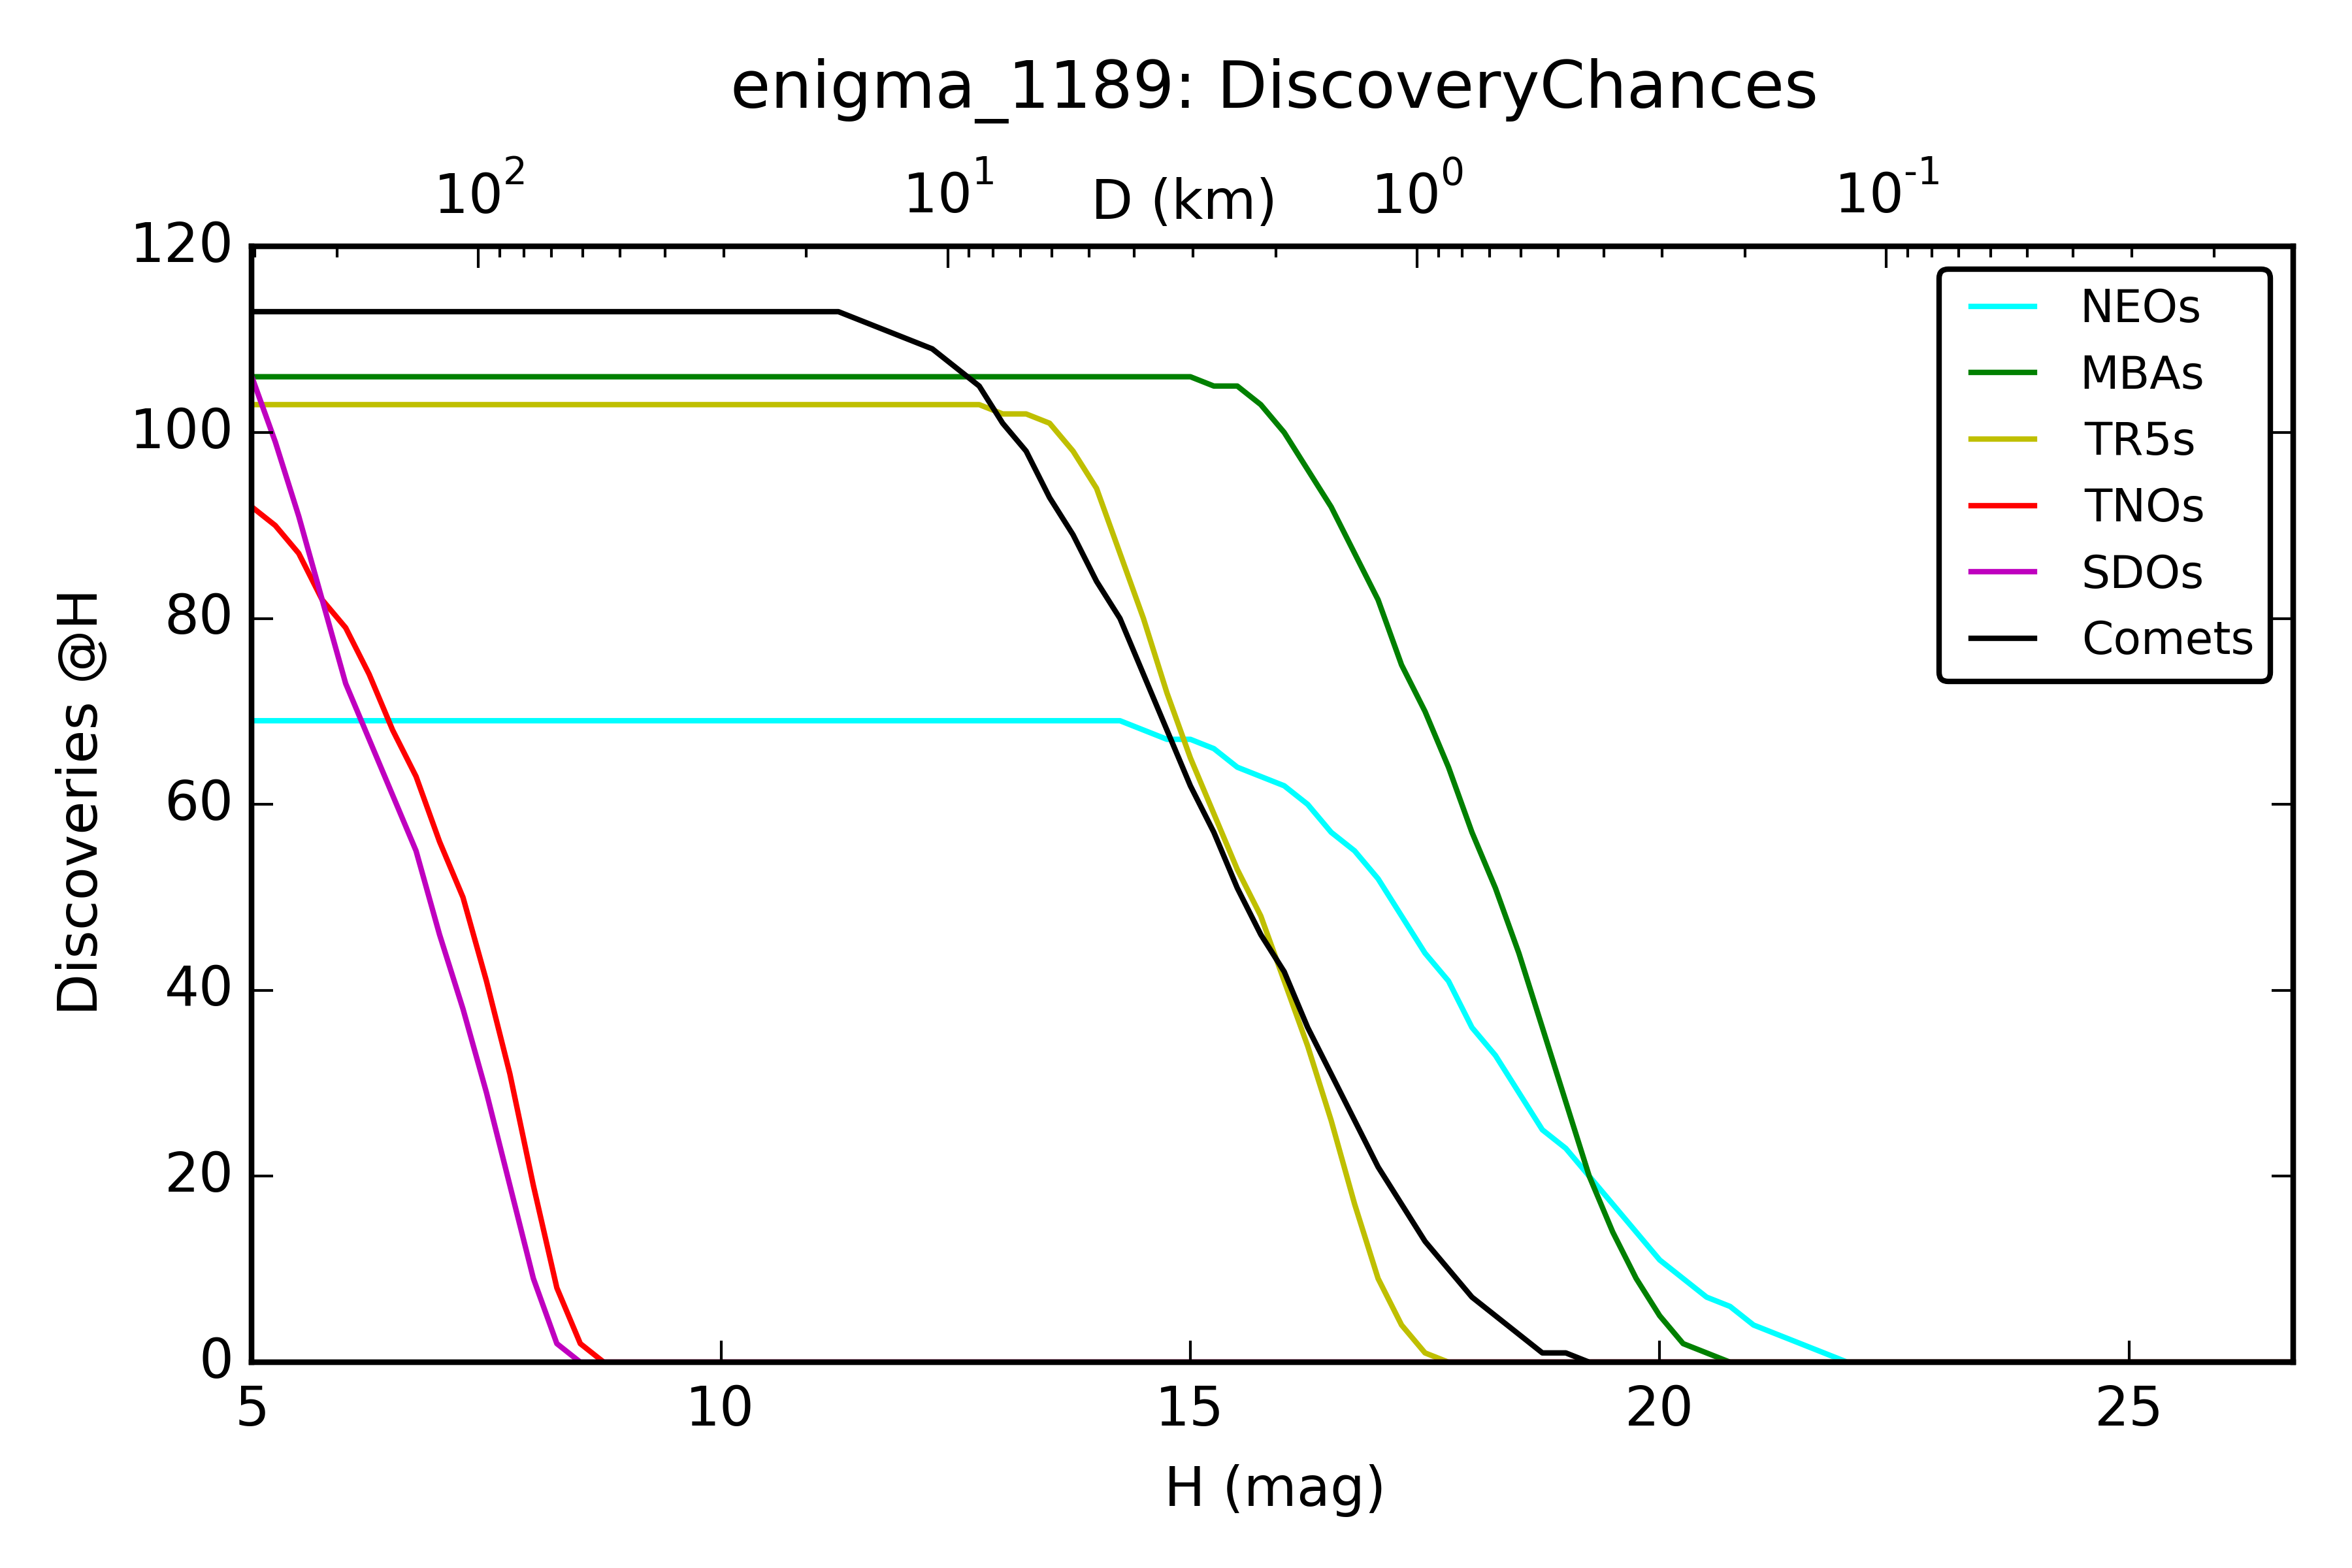
\includegraphics[width=3.5in]{figs/solarsystem/discoverychances}
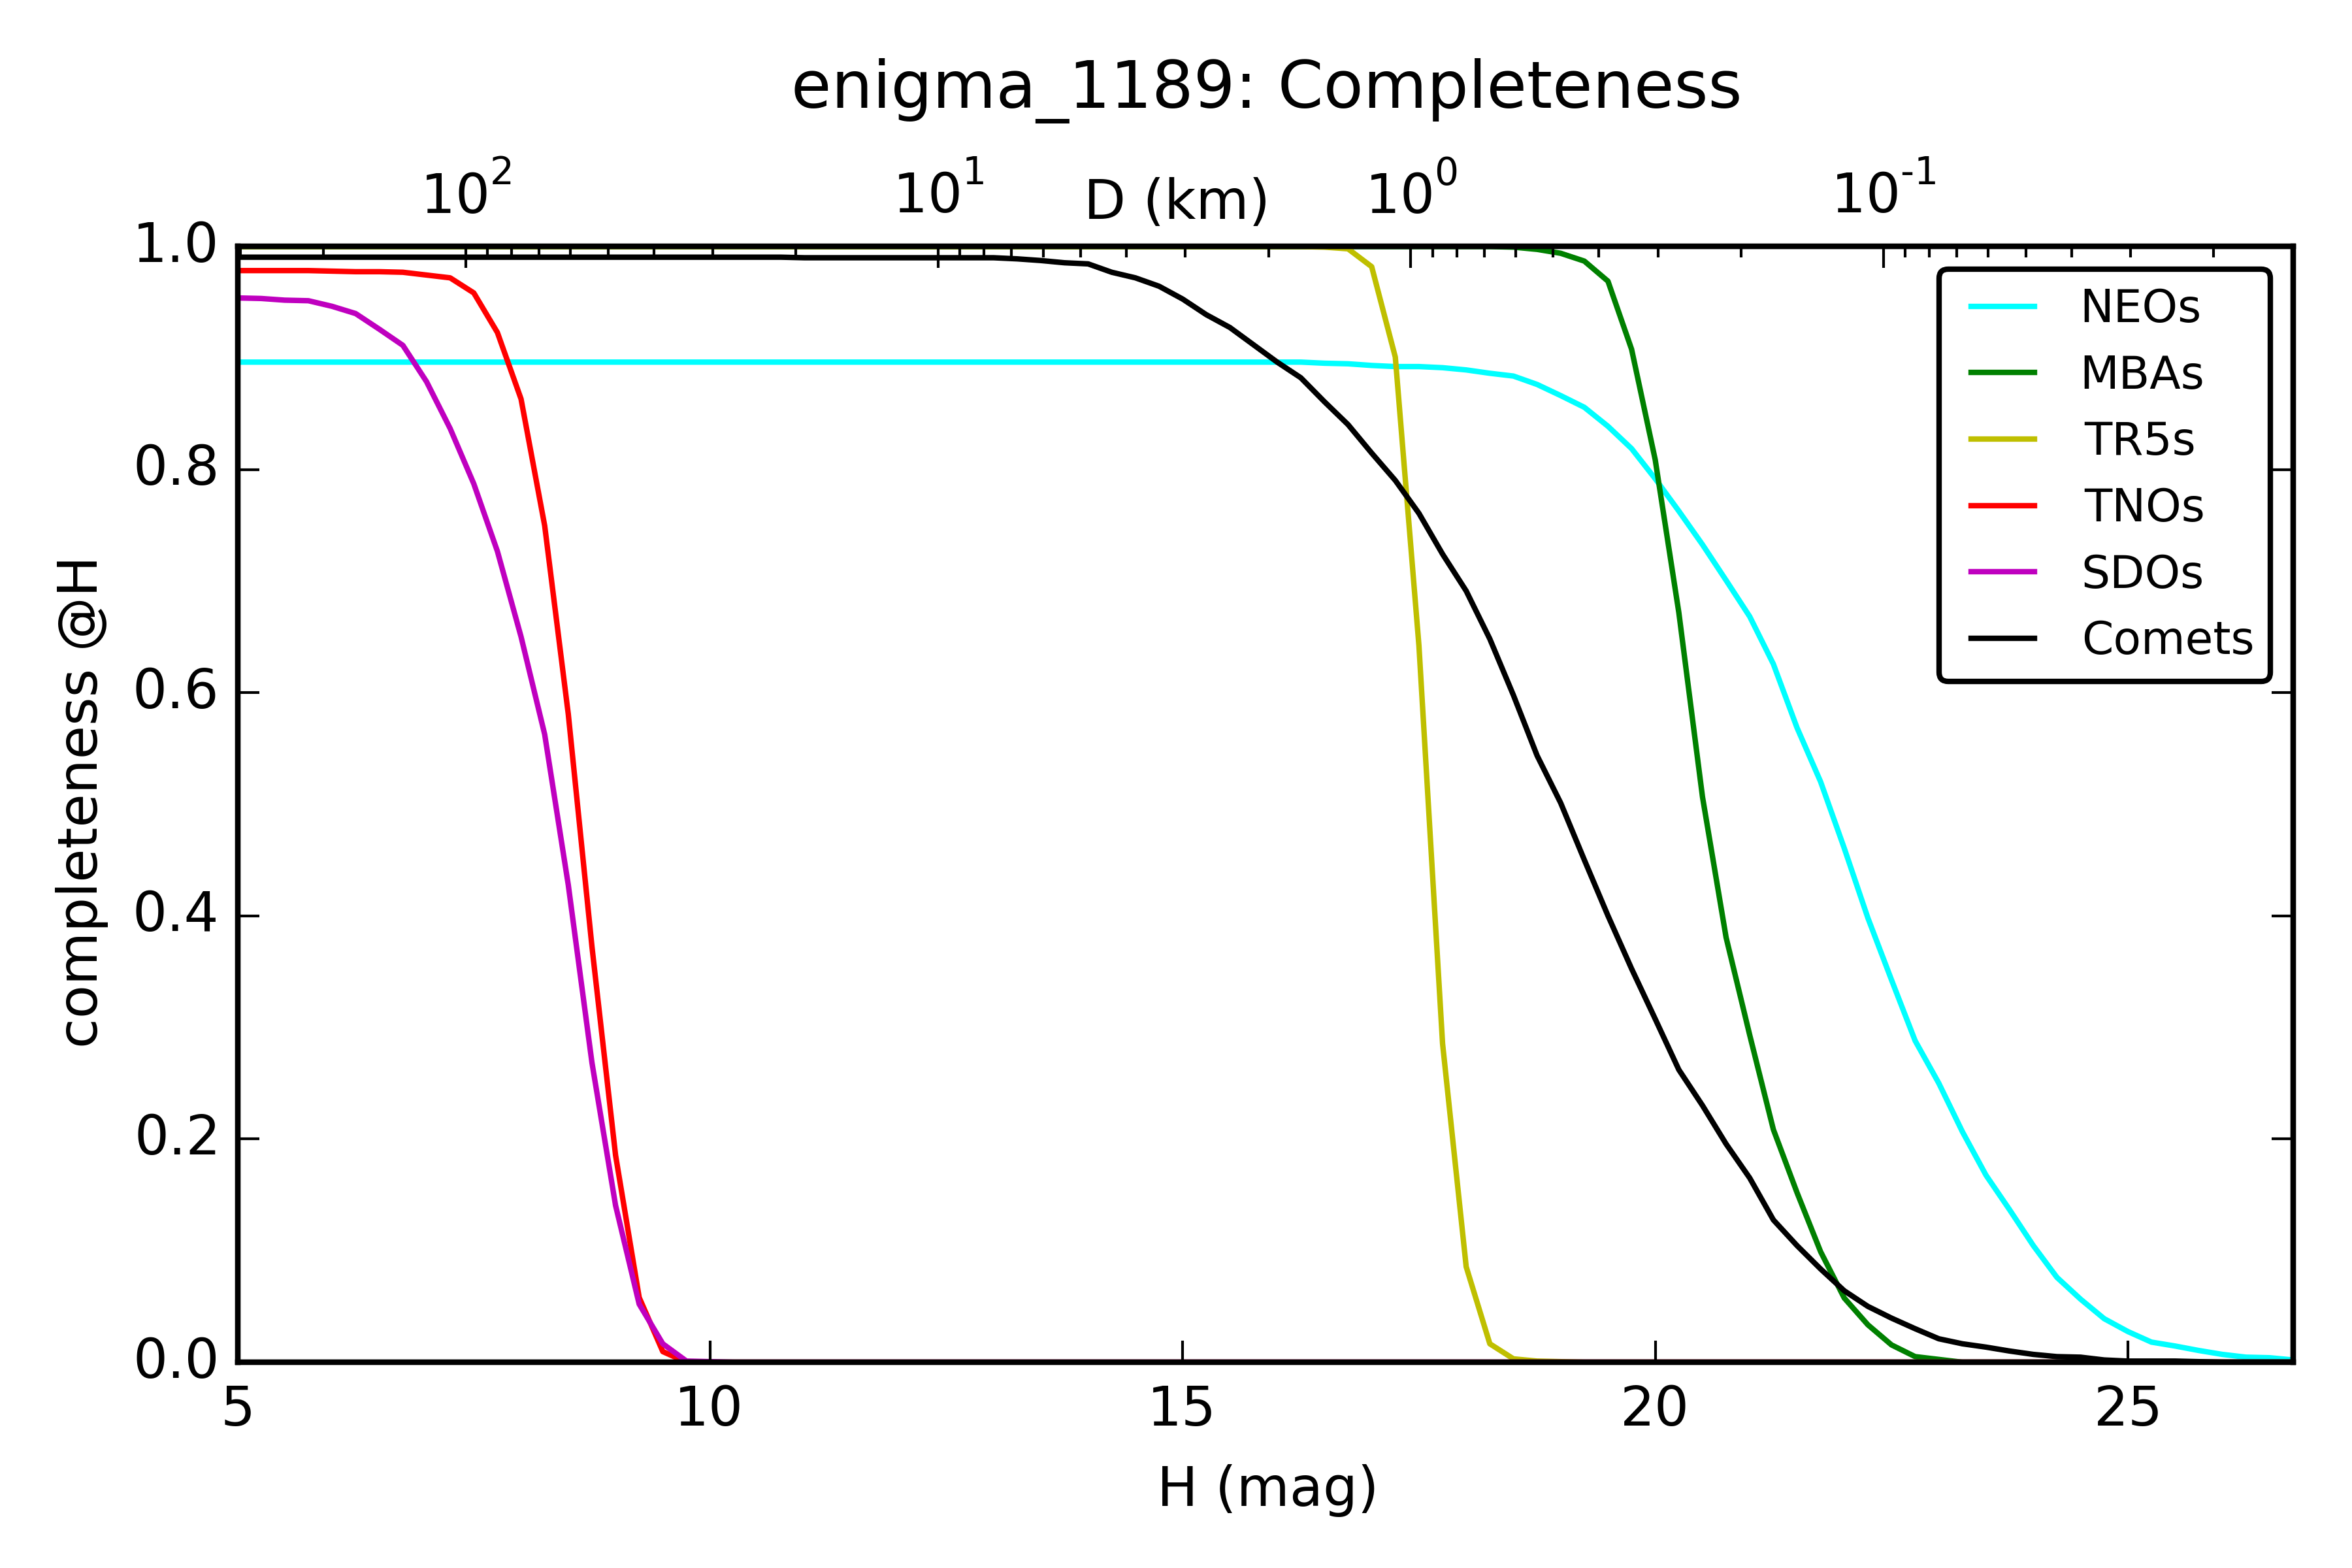
\includegraphics[width=3.5in]{figs/solarsystem/completeness}
\caption{Left: Number of discovery chances as a function of H
  (median value for all objects), assuming the minimum criteria for
  discovery - 2 visits per night within 90 minutes, repeated for 3
  nights within 15 days. Right: Resulting completeness across the
  entire population, assuming that only 1 discovery opportunity is
  required to `discover' each object. 
\label{standard_discovery}}
\end{figure}

Add table?


% --------------------------------------------------------------------

\subsection{Discussion}
\label{sec:\secname:discussion}

Add minimum completeness levels from solar system requirements
document



Discussion: what risks have been identified? What suggestions could be
made to improve this science project's figure of merit, and mitigate
the identified risks?



% ====================================================================

\section{Orbital Accuracy}
\def\secname{\chpname:orbits}\label{sec:\secname}


A short preamble goes here. What's the context for this science
project? Where does it fit in the big picture?

% --------------------------------------------------------------------

\subsection{Target measurements and discoveries}
\label{sec:\secname:targets}

Describe the discoveries and measurements you want to make.

Now, describe their response to the observing strategy. Qualitatively,
how will the science project be affected by the observing schedule and
conditions? In broad terms, how would we expect the observing strategy



% --------------------------------------------------------------------

\subsection{Metrics}
\label{sec:\secname:metrics}

Quantifying the response via MAF metrics: definition of the metrics,
and any derived overall figure of merit.


% --------------------------------------------------------------------

\subsection{OpSim Analysis}
\label{sec:\secname:analysis}

OpSim analysis: how good would the default observing strategy be, at
the time of writing for this science project?


% --------------------------------------------------------------------

\subsection{Discussion}
\label{sec:\secname:discussion}

Discussion: what risks have been identified? What suggestions could be
made to improve this science project's figure of merit, and mitigate
the identified risks?


% ====================================================================

\section{Detecting Activity}
\def\secname{\chpname:activity}\label{sec:\secname}


A short preamble goes here. What's the context for this science
project? Where does it fit in the big picture?

How secure is the orbit - is it going to hit us?
Libration amplitude distribution for TNOs?
Can we find it after X years for further study?
Can we identify the source region for NEOs within the main belt?

% --------------------------------------------------------------------

\subsection{Target measurements and discoveries}
\label{sec:\secname:targets}

Describe the discoveries and measurements you want to make.

Now, describe their response to the observing strategy. Qualitatively,
how will the science project be affected by the observing schedule and
conditions? In broad terms, how would we expect the observing strategy
to be optimized for this science?


% --------------------------------------------------------------------

\subsection{Metrics}
\label{sec:\secname:metrics}

Quantifying the response via MAF metrics: definition of the metrics,
and any derived overall figure of merit.


% --------------------------------------------------------------------

\subsection{OpSim Analysis}
\label{sec:\secname:analysis}

OpSim analysis: how good would the default observing strategy be, at
the time of writing for this science project?


% --------------------------------------------------------------------

\subsection{Discussion}
\label{sec:\secname:discussion}

Discussion: what risks have been identified? What suggestions could be
made to improve this science project's figure of merit, and mitigate
the identified risks?

Different discussion / risks for each science case within this general metric?

% ====================================================================

\section{Measuring lightcurves/rotation periods}
\def\secname{\chpname:lightcurves}\label{sec:\secname}

Two Solar System science projects require
a series of photometric measurements. These
are (1) measuring lightcurves and therefore
shapes of minor bodies and (2) measuring
the colors and therefore compositions of
minor bodies. This section and the next describe
the science and the metrics for these
experiments.

% --------------------------------------------------------------------

\subsection{Target measurements and discoveries}
\label{sec:\secname:targets}

In general, minor bodies are aspherical,
and therefore observations of those bodies
produce lightcurves with non-zero amplitudes.
Constant monitoring of such a body would
reveal the detailed lightcurve, which can
be inverted to derive the effective observed
shape at that epoch.
Observations
over multiple epochs allow for observations
at different aspects, which can be used to
determine the three dimensional shape and pole
orientation of the minor body. All of this
information can be used to understand,
broadly, the orbital and physical evolution
of minor bodies in the Solar System.

LSST observations of minor bodies in the Solar System
will not, however, necessarily be dense in time
(with the exception of observations made in
Deep Drilling Fields; see below).
Therefore, lightcurves of minor bodies must
be combined across arbitrary rotational phase.
Without knowing the phase, the amplitude of
the lightcurve (a proxy for
asteroid shape) can simply be determined.
More complicated lightcurve inversion analysis
xxx ref xxx
can be carried out, given a sufficient number
of points.


% --------------------------------------------------------------------

\subsection{Metrics}
\label{sec:\secname:metrics}

The metric for lightcurve analysis
is therefore related to the number
of observations. The specific requirement
is
at least $\sim$100 measurements of an asteroid over
$\sim$years,
calibrated with a photometric accuracy of
$\sim$5\% (SNR=20)
or better. In these cases,
a coarse shape model can be derived.
The sparse data inversion gives correct results for both fast (0.2--2~h) and slow ($>$24~h) rotators (Durech et al.\ 2007, IAUS).



% --------------------------------------------------------------------

\subsection{OpSim Analysis}
\label{sec:\secname:analysis}

The present default OpSim does pretty well for this project.
Our estimate from existing metrics is that some $10^5$~main
belt asteroids will be observed $>$500~times in the 
nominal survey. 



% --------------------------------------------------------------------

\subsection{Discussion}
\label{sec:\secname:discussion}

The success of this experiment is predicated
on the idea that MOPS will work as advertised, 
that is, that the linking of tracklets and tracks
will be successful, so that each object's photometric
time series can be identified.

% ====================================================================

\section{Measuring colors}
\def\secname{\chpname:colors}\label{sec:\secname}

The varying compositions of asteroids result
in a range of optical colors. Sloan filters
in general are sufficiently diagnostic to
discriminate among different compositional
class xxx ref xxx. Therefore, when a Solar System
minor body is observed in griz (Solar System
objects are generally quite faint in u band
and many fewer will be detected; Y band xxx),
the color can be used to determine the composition
and, downstream, composition as a function of
asteroid size, family membership, orbital
elements, or many other parameters.

One obstacle to determining asteroid colors
is that asteroid rotation periods are
on the order of 2--20~hours, so that after
an initial measurement all further
measurements (in the same filter, or other
filters) are obtained at an arbitrary rotational
phase.
However, as described above, asteroid lightcurves
in a single band (presumably r band, which
will likely have the most detections) can be
derived. Any observing of that asteroid
in a different filter can be corrected
for the derived lightcurve brightness
offset at the time of the non-r band observation.
The intrinsic color of the asteroid can therefore
be measured.

% --------------------------------------------------------------------

\subsection{Target measurements and discoveries}
\label{sec:\secname:targets}


The metric of interest is the number
of observations in each band. If an asteroid has
more than $\sim$100 observations in r band,
then the lightcurve can be determined, and the
color can then be derived. The fidelity of the color
will depend on the number of measurements in
each band with SNR$>$20 (giving colors good to
5\%).



% --------------------------------------------------------------------

\subsection{Metrics}
\label{sec:\secname:metrics}

The metric of interest is the number
of observations in each band. If an asteroid has
more than $\sim$100 observations in r band,
then the lightcurve can be determined, and the
color can then be derived. The fidelity of the color
will depend on the number of measurements in
each band with SNR$>$20 (giving colors good to
5\%).



% --------------------------------------------------------------------

\subsection{OpSim Analysis}
\label{sec:\secname:analysis}

OpSim analysis: how good would the default observing strategy be, at
the time of writing for this science project?


% --------------------------------------------------------------------

\subsection{Discussion}
\label{sec:\secname:discussion}

Discussion: what risks have been identified? What suggestions could be
made to improve this science project's figure of merit, and mitigate
the identified risks?



% ====================================================================

\section{Deep Drilling Observations}
\def\secname{\chpname:dd}\label{sec:\secname}

Deep drilling observations provide the opportunity, via digital
shift-and-stack techniques, to discover Solar System Objects fainter
than the individual image limiting magnitude. These fainter objects
will be smaller, more distant, or lower albedo (or some combination of these)
than the general population found with individual images. Discovering smaller
objects is useful for constraining the size distribution to smaller
sizes; this provides constraints for collisional models and insights
into planetesimal formation. More distant objects are interesting in
terms of extending our understanding of each population over a wider
range of space; examples would be discovering very distant
Sedna-like objects or comets at larger distances from the Sun before
the onset of activity. Lower albedo objects may be useful to
understand the distribution of albedos, particularly to look for
trends with size.

Variations on the basic method of shift-and-stack have been used to
detect faint TNOs XXX Allen, Bernstein, Gladman, Fuentes, ?
XXX. Computational limitations on these methods mean that, roughly
and in general for images taken at opposition, images taken over the timespan of about an hour can be
combined and searched for main belt asteroids, and images taken over
the timespan of about 3 days can be combined and searched for more
distant objects like TNOs.

With extragalactic deep drilling fields as in the baseline enigma\_1189
run, where observations are taken in a series of filters (g, r, and i
would be useful for this purpose) each night, every three or four
days, we could use shift-and-stack to coadd the 50 images obtained in
gri bandpasses in a single night. This would allow detection of
objects about 2 magnitudes fainter than in the regular survey, or
approximately $r=26.5$.  This is cool and a range of ecliptic
latitudes is interesting.  But, we would like to do better.

Recap solar system DD white paper.

Describe how we will evaluate DD proposal, with TNO population +
estimate on number of times objects observed (but not doing actual
shift-and-stack). Need large-i populations to test if useful, probably.


\navigationbar

% ====================================================================


% --------------------------------------------------------------------

\chapter[The Galaxy]{The Galaxy}
\def\chpname{galaxy}\label{chp:\chpname}

\noindent {\it
Will Clarkson, Kathy Vivas, Peregrine McGehee, and others to follow
}

% --------------------------------------------------------------------

\section{Introduction}
\def\secname{intro}\label{sec:\secname}

% WIC 2015-08-21 15:00: lots of edits to the intro text to refocus the
% document a bit more usefully.

LSST will significantly advance Milky Way science, on lengthscales
from the galactic halo and local volume, right down to sensitive
surveys for faint nearby objects to uncover the true state of the
Solar Neighborhood.
%The broad reach of the Milky Way science
%cases is nicely summarized in Section 2.1.4 of Ivezic et al. (2008
%arXiv 0805.2366).
%\begin{itemize}
%\item What is the detailed structure and accretion history of the Milky Way?
%\item What are the fundamental properties of all the stars within 300 pc of the Sun?
%\end{itemize}
Much more detail about most of these science cases, and specific
science questions to be answered, can be found in the LSST Science
Book (particularly chapters 6 and 7) and Ivezic et al. (2008 arXiv
0805.2366, in particular Sections 2.1.4 and 4.4); in this chapter we
(aim to) present metrics that will allow various observing strategies
to be quantitatively assessed in terms of their impact on science
cases falling under the general rubric of ``The Milky Way.''  

Our intention is to decouple the technical issue of coverage on-sky
from the science accomplished; for example, if a science case includes
regions both inside and outside of the ``Wide-Fast-Deep'' (WFD)
survey, then the metric for a particular science case should produce a
quantitative assessment of the science outcome no matter what the
distribution of pointings on the sky actually was. As a result, issues
to do with areal coverage (for example, whether a census of all nearby
brown dwarfs that neglects ``low-latitude'' fields towards the inner
Galaxy, is scientifically unacceptable) should in theory fall out as a
result of the metrics assessment process.

This chapter is organized as follows. In Section \ref{sec:GeneralMW}
we point out some general considerations specific to much of the Milky
Way science area that we recommend MW scientists bear in mind when
considering metrics. Because of the large diversity of science cases,
Section \ref{sec:SummaryTableMW} presents the essential aspects of
each science case, expressed in terms of observational goals and
tracer population. Science cases dominated by in-plane observations
are presented first in Table X, as the observing strategy for in-plane
observations is currently far from resolved. Then Table Y in this
section presents the vital statistics for science cases covered by
Wide-Fast-Deep. Sections
\ref{sec:MW_spatial_structure}-\ref{sec:MW_localvolume} then present
the metrics and their evaluations for MW science cases. Finally,
section \ref{sec:MW_future_work} points the way to anticipated future
improvements to this living document in light of expected precursor data.

\section{Some general considerations for Milky Way metrics}
\def\secname{GeneralMW}\label{sec:\secname}

Many of the Milky Way science cases involve Galactic Plane
observations almost exclusively. At the time of writing (late August
2015), even the broad parameters of in-plane observations remain to be
decided (for example the number of exposures per-filter).

Before launching into the specifics of metrics per-science case, we
point out some general factors that are likely to obtain for Milky Way
science (all over the sky), which we encourage the reader to
incorporate into their thinking when considering possible
metrics. [Language will change as metrics are produced.]

We currently envisage these to be implemented as methods that a given
science metric would call as part of its chain of evaluation.

{\it 1. Observing the ``foreground:''} By the standards of LSST's
Wide-Fast-Deep survey, many if not most of the objects of interest to
Milky Way science are close enough that they will saturate under the
Wide-Fast-Deep cadence, or will be impacted by bright foreground
objects. With LSST's saturation limit at 15 second exposure in the
neighborhood of $r \sim 17$~({\bf need confirmation!}), metrics should
include in their chain of evaluation, some sensitivity to at least the
following implications of foreground observation:

\begin{itemize}
  \item The upper limit on brightness for which measurements can be made that are sufficiently accurate for a given science case;
  \item The loss in discovery efficiency due to charge bleeds from objects unrelated to the targets for a given science case.
\end{itemize}

The discovery efficiency metric may correlate with existing
first-order metrics already presented elsewhere; for example, the
range of position angles for a field will likely correlate with the
discovery efficiency in the presence of charge bleeds, as a wider
range of position-angles will reduce the number of exposures in which
a given faint target lies underneath the charge bleed from one very
bright foreground object. Or, a given dithering strategy might
increase discovery efficiency due to pathological, very close, very
bright objects being moved into chip-gaps during some of the dithers.

(One suggested observing configuration for the Plane to mitigate the
impact of both of these factors, is to split the exposures per pair
into unequal-length exposures; perhaps $(1 \times 1s + 1\times 10s)$,
to ensure that nearly every object has an unsaturated exposure in
nearly every field. Although we do not wish to suggest a large array
of observing strategies at this stage, we do recommend that this
option be simulated for in-plane observations.)

{\it 2: Crowding and seeing:} Metrics for in-plane science must
incorporate the impact of spatial confusion on both photometric and
astrometric measurements. Both of these depend on seeing. More work
remains to be done on the level of sophistication necessary in these
considerations; for example, when considering relative proper motion
precision, the spatial density of reference stars at similar
brightness to the object whose proper motion is desired (to mitigate
magnitude-dependent PSF effects like the ``fatter-brighter'' effect)
will in principle impact the proper motion precision attainable. The
size of the impact of this effect on proper motion precision should be
determined.

{\it 3: Relative and absolute metrics:} Because even the first-order
observation parameters for in-plane observations are somewhat
unconstrained, metrics should be sensitive to differences in overall
allocation as well as by comparison to the ideal strategy within an
allocation. For example, the way in which observations are distributed
within a time baseline is not very impactful to many science cases if
that baseline is only three years long for OpSim algorithmic reasons!
(For example, OpSim might move all the exposures in a galactic plane
science case into the first three years to finish short projects
early, which would be a disaster for cases that require a long time
baseline.)

\section{Summary table of Milky Way science cases}
\def\secname{SummaryTableMW}\label{sec:\secname}

Here we present a quick-look summary of the Milky Way science cases
to-date, with measurement type and tracer population indicated where
appropriate. This communicates the importance of certain objects and
certain regimes to Milky Way science. Given the considerations
outlined in Section \ref{sec:GeneralMW}, this overview is split in two
tables: Table 1 shows science cases for the five main science cases we
have identified for metric development, while while Table Y summarizes
the rest in terms of tracers and simple scaling relations (the
majority of which can safely assume SRD performance numbers).

{\bf All those bullet points from v1 of this chapter are condensed and summarized in these tables.}

[Table 1 - measurements and tracers for the five main science cases requiring new metrics.]

[Table 2 - Milky Way science cases not in Table 1; scaling relations from other metrics.]

({\it Hierarchical metrics (e.g. github Issue \#79):} since others are
developing detailed metrics for fine-grained issues of detectability,
in this Chapter we focus our candidate metrics mostly on high-level
metrics that might call the variability metrics as functions.) 

The following sections describe observing metrics for Milky Way
science cases. These have signficant (but not exclusive)
observation-sets in or towards the Plane. If your science case is not
mentioned below, it should be mentioned concisely in Table 2.


% Subsection filenames all start with ``MW'' in violation of Phil's
% advice to avoid chapter-specific names. This is to avoid namespace
% collision between ``microlensing'' for AGN and ``microlensing'' in
% the MW, for example!

Section \ref{sec:MW_spatial_structure}: Spatial Structure of the Milky Way Galaxy, including the plane, bulge, halo and local volume;

Section \ref{sec:MW_metallicity_mapping}: Galactic photometric metallicity mapping; 

Section \ref{sec:MW_SFH}: Star formation history of the Milky Way;

Section \ref{sec:MW_Dust}: Dust in the Milky Way plane;

Section \ref{sec:MW_microlensing} Microlensing;

% There may be one more section here: stellar populations of interest
% with unknown scale-heights. Chuck Claver's white dwarf pulsator
% project might be of interest here, among others.

%{\it Milky Way science cases but mostly in Wide-Fast-Deep:}

%Section \ref{sec:solarneighborhood} The Solar Neighborhood;

%Section \ref{sec:starclusters} Star Clusters in the Milky Way;

%Section \ref{sec:halostructure} Halo structure and populations;

%Section \ref{sec:localvolume} The Local Volume

[As of 2015-08-21, the .tex files for these subsections are mostly
  empty shells. Content to follow.]

[To be resolved: how to ensure Solar Neighborhood science is best represented. Does this deserve a sixth section?]

\input{MilkyWay/MW_spatial_structure.tex}
% ====================================================================
%+
% SECTION:
%    section-name.tex  % eg lenstimedelays.tex
%
% CHAPTER:
%    chapter.tex  % eg cosmology.tex
%
% ELEVATOR PITCH:
%    Explain in a few sentences what the relevant discovery or
%    measurement is going to be discussed, and what will be important
%    about it. This is for the browsing reader to get a quick feel
%    for what this section is about.
%
% COMMENTS:
%
%
% BUGS:
%
%
% AUTHORS:
%    Phil Marshall (@drphilmarshall)  - put your name and GitHub username here!
%-
% ====================================================================

\section{Metallicity and age mapping in the Milky Way}
\def\secname{MW_metallicity_mapping}\label{sec:\secname} % For example, replace "keyword" with "lenstimedelays"

\noindent{\it Author Name(s)} % (Writing team)

% This individual section will need to describe the particular
% discoveries and measurements that are being targeted in this section's
% science case. It will be helpful to think of a ``science case" as a
% ``science project" that the authors {\it actually plan to do}. Then,
% the sections can follow the tried and tested format of an observing
% proposal: a brief description of the investigation, with references,
% followed by a technical feasibility piece. This latter part will need
% to be quantified using the MAF framework, via a set of metrics that
% need to be computed for any given observing strategy to quantify its
% impact on the described science case. Ideally, these metrics would be
% combined in a well-motivated figure of merit. The section can conclude
% with a discussion of any risks that have been identified, and how
% these could be mitigated.

A short preamble goes here. What's the context for this science
project? Where does it fit in the big picture?

% --------------------------------------------------------------------

\subsection{Target measurements and discoveries}
\label{sec:keyword:targets}

Describe the discoveries and measurements you want to make.

Now, describe their response to the observing strategy. Qualitatively,
how will the science project be affected by the observing schedule and
conditions? In broad terms, how would we expect the observing strategy
to be optimized for this science?


% --------------------------------------------------------------------

\subsection{Metrics}
\label{sec:keyword:metrics}

Quantifying the response via MAF metrics: definition of the metrics,
and any derived overall figure of merit.


% --------------------------------------------------------------------

\subsection{OpSim Analysis}
\label{sec:keyword:analysis}

OpSim analysis: how good would the default observing strategy be, at
the time of writing for this science project?


% --------------------------------------------------------------------

\subsection{Discussion}
\label{sec:keyword:discussion}

Discussion: what risks have been identified? What suggestions could be
made to improve this science project's figure of merit, and mitigate
the identified risks?


% ====================================================================

\navigationbar

% ====================================================================
%+
% SECTION:
%    MW_SFH.tex
%
% CHAPTER:
%    galaxy.tex
%
% ELEVATOR PITCH:
%
%-
% ====================================================================

\section{Star Formation History of the Milky Way}
\def\secname{MW_SFH}\label{sec:\secname}

\credit{pmmcgehee}

\label{sec:\secname:targets}

% This individual section will need to describe the particular
% discoveries and measurements that are being targeted in this section's
% science case. It will be helpful to think of a ``science case" as a
% ``science project" that the authors {\it actually plan to do}. Then,
% the sections can follow the tried and tested format of an observing
% proposal: a brief description of the investigation, with references,
% followed by a technical feasibility piece. This latter part will need
% to be quantified using the MAF framework, via a set of metrics that
% need to be computed for any given observing strategy to quantify its
% impact on the described science case. Ideally, these metrics would be
% combined in a well-motivated figure of merit. The section can conclude
% with a discussion of any risks that have been identified, and how
% these could be mitigated.

LSST gives the opportunity to survey extensive areas
around star formation regions in the Southern hemisphere. Among
others, it would allow to study the Initial Mass Function down to the
sub-stellar limit across different environments. Young stars are
efficiently identified by their variability.

Section 8.10.2 in the LSST Science Book (p298--299) provides a
  thorough scientific motivation for the characterization of young
  stars through variability, including discussion of the observational
  signatures of the diverse physical phenomena driving observed time
  variability. The general observable is strong, irregular flaring
  across the entire $ugrizy$~bandpass of LSST. Flaring can last from
  minutes to years, and at amplitudes from a few tenths to several
  magnitudes.

% WIC - the following para has been removed since it's already present
% verbatim at the end of Section 8.10.2 in the LSST Science Book.

%LSST will increase the sample size for detailed follow-up observations
%due its ability to survey star formations at large heliocentric
%distances and to detect variability in embedded and highly extincted
%young objects that would otherwise be missed in shallower
%surveys. During its operations LSST will also provide statistics on
%the durations of high states, for at least one important tracer
%population (the shorter-duration EXor variables).

% --------------------------------------------------------------------

\subsection{Target measurements and discoveries}
\label{sec:\secname:targets}

The nature of the variability in young stars changes with evolutionary
status. For the youngest stars still undergoing significant mass
accretion, FU Orionis and related outbursts can occur due to
circumstellar disk instabilities. As the natal environment dissipates
and the accretion rates drops, the stars take on a Classical T Tauri
appearance where the variability is primarily due to changes in the
accretion flow and rotational modulation of hot spots resulting from
accretion shocks on the protostellar photosphere. Also present are the
signature of cool spots arising from strong magnetic fields. This cool
spot rotational modulation is responsible for the variability in the
disk-less, and older, weak-line T Tauri stars.

Of particular interest are the FUor and EXor variables, which are
  named after the prototype objects FU Orionis \citep{hartmann96}
  and EX Lupi \citep{herbig01} respectively, and for which
  only a relatively small number of examples are known. In these
  pre-main sequence objects, eruptive outbursts of up to 6 magnitudes
  have been observed, with high state durations from years to
  decades. In addition to triggering follow-up observations, LSST
  should be able to set the first population constraints on the
  duration of high states, particularly for the short end of the
  timescale distribution for these eruptive variables.


% \new{(WIC: Material already in LSST Science Book removed.)}


%{\bf CTTS and WTTS material goes here.}

%Here are the references cited above:\\
%Hartmann \& Kenyon 1996, ARA\&A, 34, 207 \\
%Herbig et al. 2001, PASP, 113, 1547 \\
%Herbig 1977, ApJ, 217, 693 \\
%Aspin et al. 2009, ApJ, 692L, 67 \\
%Hodapp et al. 1996, ApJ, 468, 861 \\
%McGehee et al. 2004, ApJ, 616, 1058 \\


%Describe the discoveries and measurements you want to make.

%Now, describe their response to the observing strategy. Qualitatively,
%how will the science project be affected by the observing schedule and
%conditions? In broad terms, how would we expect the observing strategy
%to be optimized for this science?


% --------------------------------------------------------------------

\subsection{Metrics}
\label{sec:\secname:metrics}

In order to assess the ability of LSST to 1) identify and 2) classify
Young Stellar Objects we need to quantify the variability timescales
and amplitudes of both Class I/II (stars with disks, including
Classical T Tauris) and Class III (Weak-line T Tauris).  Inclusion of
eruptive variables (FUor/EXor) is appropriate as well.

In brief, Weak-line T-Tauris are quasi-periodic with amplitudes of 0.1
to 0.3 mag and periods 1 to $\sim$15 days, so their variability is
comparable to that of $\gamma$ Dor stars. Given the temporal evolution
of cool spots, a period recovery analysis such as shown for RR Lyrae
stars is likely difficult.  The embedded systems and Classical T
Tauris are irregular variables but have been shown to have distinctive
colors due to extinction and the ultraviolet and blue excess arising
from accretion shocks.

\autoref{table:pseudoForExor} shows a possible Figure of Merit for the
recovery by LSST of the distribution of EXor high-state duration in
outburst.


\begin{table}
\small
\begin{tabular}{c p{12cm}}
& {\it Figure of Merit for recovery of EXor high--state duration distribution}\\
\hline
1.  & Produce ASCII lightcurve for eruptive outburst \\
2.  & Initialise large array to store the maps of fraction detected as a function of duration and amplitude. \\
2.  & for {\it duration T} in range \{min, max\}:  \\
3.  & ~~~~ for {\it amplitude A} in range \{min, max\}: \\
4.  & ~~~~~~~~~~ run {\tt mafContrib/transientAsciiMetric} \\
5.  & ~~~~~~~~~~ store the spatial map of the fraction detected for this (A, T) pair \\
6.  & Initialise master arrays to hold the run of duration distribution measurements.\\
7. & Produce distribution of high--state durations and amplitudes from which the simulations will be drawn. \\
8.  & for {\it iDraw} in range \{1, nDraws\}:\\
9.  & ~~~~ construct model population with input duration distribution \\
10.  & ~~~~ Apply the stored metrics from 2-5 to measure fraction recovered \\
11.  & ~~~~ Characterize the duration distribution for this draw \\
12. & ~~~~ Fill the {\it iDraw}'th entry in the master arrays. \\
13. & {\bf FoM 1:} Compute the median and variance of the upper/lower quintiles. \\
14. & {\bf FoM 2:} Evaluate the bias between recovered and input high-state duration. \\
\hline
\end{tabular}
\caption{\new{Steps for Figure of Merit recovering the distribution
  for the duration of EXor high states. See Section \ref{sec:MW_SFH:targets} }}
\label{table:pseudoForExor}
\end{table}


% --------------------------------------------------------------------

%\subsection{OpSim Analysis}
%\label{sec:\secname:analysis}

%OpSim analysis: how good would the default observing strategy be, at
%the time of writing for this science project?

% --------------------------------------------------------------------

\subsection{Discussion}
\label{sec:\secname:discussion}

Galactic star formation regions are largely found at low Galactic
latitudes or within the Gould Belt structure. As such study of young
stars with LSST is closely tied to other science goals concerning the
Milky Way Disk and is subject to the concerns of both crowded field
photometry and the observing cadence along the Milky Way.

The embedded and Classical T Tauri stars also undergo significant and
rapid color changes due to accretion processes. The ability of LSST to
track these variations in color could be limited by the interval
between filter changes.

% ====================================================================
%
% \subsection{Conclusions}
%
% Here we answer the ten questions posed in
% \autoref{sec:intro:evaluation:caseConclusions}:
%
% \begin{description}
%
% \item[Q1:] {\it Does the science case place any constraints on the
% tradeoff between the sky coverage and coadded depth? For example, should
% the sky coverage be maximized (to $\sim$30,000 deg$^2$, as e.g., in
% Pan-STARRS) or the number of detected galaxies (the current baseline but
% with 18,000 deg$^2$)?}
%
% \item[A1:] ...
%
% \item[Q2:] {\it Does the science case place any constraints on the
% tradeoff between uniformity of sampling and frequency of  sampling? For
% example, a rolling cadence can provide enhanced sample rates over a part
% of the survey or the entire survey for a designated time at the cost of
% reduced sample rate the rest of the time (while maintaining the nominal
% total visit counts).}
%
% \item[A2:] ...
%
% \item[Q3:] {\it Does the science case place any constraints on the
% tradeoff between the single-visit depth and the number of visits
% (especially in the $u$-band where longer exposures would minimize the
% impact of the readout noise)?}
%
% \item[A3:] ...
%
% \item[Q4:] {\it Does the science case place any constraints on the
% Galactic plane coverage (spatial coverage, temporal sampling, visits per
% band)?}
%
% \item[A4:] ...
%
% \item[Q5:] {\it Does the science case place any constraints on the
% fraction of observing time allocated to each band?}
%
% \item[A5:] ...
%
% \item[Q6:] {\it Does the science case place any constraints on the
% cadence for deep drilling fields?}
%
% \item[A6:] ...
%
% \item[Q7:] {\it Assuming two visits per night, would the science case
% benefit if they are obtained in the same band or not?}
%
% \item[A7:] ...
%
% \item[Q8:] {\it Will the case science benefit from a special cadence
% prescription during commissioning or early in the survey, such as:
% acquiring a full 10-year count of visits for a small area (either in all
% the bands or in a  selected set); a greatly enhanced cadence for a small
% area?}
%
% \item[A8:] ...
%
% \item[Q9:] {\it Does the science case place any constraints on the
% sampling of observing conditions (e.g., seeing, dark sky, airmass),
% possibly as a function of band, etc.?}
%
% \item[A9:] ...
%
% \item[Q10:] {\it Does the case have science drivers that would require
% real-time exposure time optimization to obtain nearly constant
% single-visit limiting depth?}
%
% \item[A10:] ...
%
% \end{description}

% ====================================================================

\navigationbar

% ====================================================================
%+
% SECTION:
%    section-name.tex  % eg lenstimedelays.tex
%
% CHAPTER:
%    chapter.tex  % eg cosmology.tex
%
% ELEVATOR PITCH:
%    Explain in a few sentences what the relevant discovery or
%    measurement is going to be discussed, and what will be important
%    about it. This is for the browsing reader to get a quick feel
%    for what this section is about.
%
% COMMENTS:
%
%
% BUGS:
%
%
% AUTHORS:
%    Phil Marshall (@drphilmarshall)  - put your name and GitHub username here!
%-
% ====================================================================

\section{Dust in the Plane of the Milky Way}
\def\secname{MW_Dust}\label{sec:\secname} % For example, replace "keyword" with "lenstimedelays"

\noindent{\it Author Name(s)} % (Writing team)

% This individual section will need to describe the particular
% discoveries and measurements that are being targeted in this section's
% science case. It will be helpful to think of a ``science case" as a
% ``science project" that the authors {\it actually plan to do}. Then,
% the sections can follow the tried and tested format of an observing
% proposal: a brief description of the investigation, with references,
% followed by a technical feasibility piece. This latter part will need
% to be quantified using the MAF framework, via a set of metrics that
% need to be computed for any given observing strategy to quantify its
% impact on the described science case. Ideally, these metrics would be
% combined in a well-motivated figure of merit. The section can conclude
% with a discussion of any risks that have been identified, and how
% these could be mitigated.

A short preamble goes here. What's the context for this science
project? Where does it fit in the big picture?

% --------------------------------------------------------------------

\subsection{Target measurements and discoveries}
\label{sec:keyword:targets}

Describe the discoveries and measurements you want to make.

Now, describe their response to the observing strategy. Qualitatively,
how will the science project be affected by the observing schedule and
conditions? In broad terms, how would we expect the observing strategy
to be optimized for this science?


% --------------------------------------------------------------------

\subsection{Metrics}
\label{sec:keyword:metrics}

Quantifying the response via MAF metrics: definition of the metrics,
and any derived overall figure of merit.


% --------------------------------------------------------------------

\subsection{OpSim Analysis}
\label{sec:keyword:analysis}

OpSim analysis: how good would the default observing strategy be, at
the time of writing for this science project?


% --------------------------------------------------------------------

\subsection{Discussion}
\label{sec:keyword:discussion}

Discussion: what risks have been identified? What suggestions could be
made to improve this science project's figure of merit, and mitigate
the identified risks?


% ====================================================================

\navigationbar

% ====================================================================
%+
% SECTION:
%    section-name.tex  % eg lenstimedelays.tex
%
% CHAPTER:
%    chapter.tex  % eg cosmology.tex
%
% ELEVATOR PITCH:
%    Explain in a few sentences what the relevant discovery or
%    measurement is going to be discussed, and what will be important
%    about it. This is for the browsing reader to get a quick feel
%    for what this section is about.
%
% COMMENTS:
%
%
% BUGS:
%
%
% AUTHORS:
%    Phil Marshall (@drphilmarshall)  - put your name and GitHub username here!
%-
% ====================================================================

\section{Microlensing in the Milky Way with LSST}
\def\secname{MW_microlensing}\label{sec:\secname} % For example, replace "keyword" with "lenstimedelays"

\noindent{\it Author Name(s)} % (Writing team)

% This individual section will need to describe the particular
% discoveries and measurements that are being targeted in this section's
% science case. It will be helpful to think of a ``science case" as a
% ``science project" that the authors {\it actually plan to do}. Then,
% the sections can follow the tried and tested format of an observing
% proposal: a brief description of the investigation, with references,
% followed by a technical feasibility piece. This latter part will need
% to be quantified using the MAF framework, via a set of metrics that
% need to be computed for any given observing strategy to quantify its
% impact on the described science case. Ideally, these metrics would be
% combined in a well-motivated figure of merit. The section can conclude
% with a discussion of any risks that have been identified, and how
% these could be mitigated.

{\bf Note: these metrics have already been worked out in some detail
  by Gould (arXiv). We do not expect to re-invent that wheel here.}

A short preamble goes here. What's the context for this science
project? Where does it fit in the big picture?

% --------------------------------------------------------------------

\subsection{Target measurements and discoveries}
\label{sec:keyword:targets}

Describe the discoveries and measurements you want to make.

Now, describe their response to the observing strategy. Qualitatively,
how will the science project be affected by the observing schedule and
conditions? In broad terms, how would we expect the observing strategy
to be optimized for this science?


% --------------------------------------------------------------------

\subsection{Metrics}
\label{sec:keyword:metrics}

Quantifying the response via MAF metrics: definition of the metrics,
and any derived overall figure of merit.


% --------------------------------------------------------------------

\subsection{OpSim Analysis}
\label{sec:keyword:analysis}

OpSim analysis: how good would the default observing strategy be, at
the time of writing for this science project?


% --------------------------------------------------------------------

\subsection{Discussion}
\label{sec:keyword:discussion}

Discussion: what risks have been identified? What suggestions could be
made to improve this science project's figure of merit, and mitigate
the identified risks?


% ====================================================================

\navigationbar


%% ====================================================================
%+
% SECTION:
%    section-name.tex  % eg lenstimedelays.tex
%
% CHAPTER:
%    chapter.tex  % eg cosmology.tex
%
% ELEVATOR PITCH:
%    Explain in a few sentences what the relevant discovery or
%    measurement is going to be discussed, and what will be important
%    about it. This is for the browsing reader to get a quick feel
%    for what this section is about.
%
% COMMENTS:
%
%
% BUGS:
%
%
% AUTHORS:
%    Phil Marshall (@drphilmarshall)  - put your name and GitHub username here!
%    Will Clarkson (@willclarkson)
%
%-
% ====================================================================

\section{The Solar Neighborhood}
\def\secname{keyword}\label{sec:\secname} % For example, replace "keyword" with "lenstimedelays"

\noindent{\it Author Name(s)} % (Writing team)

% This individual section will need to describe the particular
% discoveries and measurements that are being targeted in this section's
% science case. It will be helpful to think of a ``science case" as a
% ``science project" that the authors {\it actually plan to do}. Then,
% the sections can follow the tried and tested format of an observing
% proposal: a brief description of the investigation, with references,
% followed by a technical feasibility piece. This latter part will need
% to be quantified using the MAF framework, via a set of metrics that
% need to be computed for any given observing strategy to quantify its
% impact on the described science case. Ideally, these metrics would be
% combined in a well-motivated figure of merit. The section can conclude
% with a discussion of any risks that have been identified, and how
% these could be mitigated.

A short preamble goes here. What's the context for this science
project? Where does it fit in the big picture?
The science projec

% --------------------------------------------------------------------

\subsection{Target measurements and discoveries}
\label{sec:keyword:targets}

Generally the cases in this science area require deep photometry,
particularly (though not exclusively) at red bandpasses, and
sufficient per-image precision and distribution of observing times in
at least one filter to measure parallax and/or proper motion. The
main-survey area is not sufficient for this science area: dedicated
observations are required for all science cases to fill in angular
coverage (apart from photometric variability of cool dwarfs).

Three representative science cases identified (more are in the Phase I
Science Roadmap):
\begin{itemize}

\item Volume-complete astrometric sample of extended Solar Neighborhood: requires parallax and proper motion, deep multi-filter photometry to classify objects.; 
\item Discovery of ultracold brown dwarfs (late-T and Y); requires very deep photometry in (i,z,Y) 

\item Photometric variability of cool dwarfs; requires sufficient time baseline sampling to chart variability; photometry at other bands to classify object. 

\end{itemize}

%Describe the discoveries and measurements you want to make.

%Now, describe their response to the observing strategy. Qualitatively,
%how will the science project be affected by the observing schedule and
%conditions? In broad terms, how would we expect the observing strategy
%to be optimized for this science?


% --------------------------------------------------------------------

\subsection{Metrics}
\label{sec:keyword:metrics}

Organized by broad science case within this area:
\begin{itemize}
\item Volume-complete astrometric sample of extended Solar Neighborhood:
  \begin{itemize}
  \item Bias and scatter in distance distribution of extended Solar Neighborhood objects;
  \item Bias and scatter in individual source $T_{eff}, \log(g)$~as a
    function of spectral type;
  \item Bias and scatter in population constrants (e.g. mass function slope) for candidate mass functions of local populations;
    \item Fraction of local-volume population recovered {\it and} correctly identified (e.g. spectral subtype error?).
  \end{itemize} 

\item Discovery of ultracold brown dwarfs (late-T/Y):
  \begin{itemize}
  \item Bias and scatter in individual source $T_{eff}, \log(g)$~as a
    function of spectral type;
    \item Bias and scatter in the brown dwarf/exoplanet (?) mass function parameters.
    \item Fraction of objects within $X$~pc from the Sun recovered {\it and} correctly identified (e.g. spectral subtype error?).
  \end{itemize}


\item Photometric variability of cool dwarfs
\begin{itemize}
  \item {\it (Note: hierarchical metric?) E.g. classification of X\% of starspot variability in local volume, which calls Variability Metric $Y$ as a method.}
\end{itemize}

\end{itemize}

%Quantifying the response via MAF metrics: definition of the metrics,
%and any derived overall figure of merit.

% --------------------------------------------------------------------

\subsection{OpSim Analysis}
\label{sec:keyword:analysis}

OpSim analysis: how good would the default observing strategy be, at
the time of writing for this science project?


% --------------------------------------------------------------------

\subsection{Discussion}
\label{sec:keyword:discussion}

One useful output of MAF for Solar Neighborhood work, will be the
extent to which the small part of the sky in front of crowded regions
in this general science area will make an impact. 

Comparison of the science metrics for cases when Galactic Plane
observations are / are not included as part of the OpSim run, will
directly address the degree to which LSST should consider Solar
Neighborhood science in its galactic plane strategy.

%Discussion: what risks have been identified? What suggestions could be
%made to improve this science project's figure of merit, and mitigate
%the identified risks?


% ====================================================================

\navigationbar

%% ====================================================================
%+
% SECTION:
%    section-name.tex  % eg lenstimedelays.tex
%
% CHAPTER:
%    chapter.tex  % eg cosmology.tex
%
% ELEVATOR PITCH:
%    Explain in a few sentences what the relevant discovery or
%    measurement is going to be discussed, and what will be important
%    about it. This is for the browsing reader to get a quick feel
%    for what this section is about.
%
% COMMENTS:
%
%
% BUGS:
%
%
% AUTHORS:
%    Phil Marshall (@drphilmarshall)  - put your name and GitHub username here!
%    Will Clarkson (@willclarkson)
%
%-
% ====================================================================

\section{Star Clusters}
\def\secname{starclusters}\label{sec:\secname} % For example, replace "keyword" with "lenstimedelays"

\noindent{\it Author Name(s)} % (Writing team)

% This individual section will need to describe the particular
% discoveries and measurements that are being targeted in this section's
% science case. It will be helpful to think of a ``science case" as a
% ``science project" that the authors {\it actually plan to do}. Then,
% the sections can follow the tried and tested format of an observing
% proposal: a brief description of the investigation, with references,
% followed by a technical feasibility piece. This latter part will need
% to be quantified using the MAF framework, via a set of metrics that
% need to be computed for any given observing strategy to quantify its
% impact on the described science case. Ideally, these metrics would be
% combined in a well-motivated figure of merit. The section can conclude
% with a discussion of any risks that have been identified, and how
% these could be mitigated.

A short preamble goes here. What's the context for this science
project? Where does it fit in the big picture?

[Star cluster leads]

%Two broad science areas {\bf [more?]}: (i) Better understanding of
%stellar populations within clusters; (ii) star clusters as tracers of
%star formation in the Galaxy, including donation to the Plane by
%dissolution

% --------------------------------------------------------------------

\subsection{Target measurements and discoveries}
\label{sec:keyword:targets}


\begin{itemize}

\item Formation history and evolution of the Milky Way as traced by star clusters

\item Better understanding of star cluster stellar populations; stellar mass function, metallicity, ages

\end{itemize}

%Describe the discoveries and measurements you want to make.

%Now, describe their response to the observing strategy. Qualitatively,
%how will the science project be affected by the observing schedule and
%conditions? In broad terms, how would we expect the observing strategy
%to be optimized for this science?


% --------------------------------------------------------------------

\subsection{Metrics}
\label{sec:keyword:metrics}

Organized by broad science case within this area:
\begin{itemize}
\item Milky Way formation and evolution as traced by star clusters (focus below on tidal dissolution $\rightarrow$~contribution of stars to the Disk by clusters):
  \begin{itemize}
    \item Radius $R$ from cluster center at which LSST becomes unable to kinematically identify cluster members (figure might be: [x,y,z] = [cluster $M_v$, concentration parameter, $R$]; rerun for different locations in the Galaxy?
      \item Sensitivity (quantified as surface brightness limit?) to tidal streams between clusters? Perhaps go broader, e.g. mass ratio or $M_v$~for tidally interacting clusters for which LSST becomes insensitive to existence of tidal tail?
        \item LSST's sensitivity to azimuthal asymmetries in the light (or mass) profile of clusters ``near'' the plane
  \end{itemize} 

\item Stellar populations within clusters; mass function, metallicity, ages
  \begin{itemize}
    \item Radius of avoidance for LSST per-filter for a catalog of
      known clusters (in-plane and out)
      \item Distance limit at which LSST becomes insensitive to stars above mass $m_{lower}$ 
  \end{itemize}

\end{itemize}

(Metrics note: all of the above are likely to be hierarchical, calling
some parameterization of photometric sensitivity vs crowding as a
method.)

Need some sort of metric for the science return on the ensemble of
globular clusters observed by LSST. If LSST doesn't go deeper than X
at latitude $|b| < Y$, what is the impact on the science?

%Quantifying the response via MAF metrics: definition of the metrics,
%and any derived overall figure of merit.

% --------------------------------------------------------------------

\subsection{OpSim Analysis}
\label{sec:keyword:analysis}

OpSim analysis: how good would the default observing strategy be, at
the time of writing for this science project?


% --------------------------------------------------------------------

\subsection{Discussion}
\label{sec:keyword:discussion}

One useful output of MAF for Solar Neighborhood work, will be the
extent to which the small part of the sky in front of crowded regions
in this general science area will make an impact. 

Comparison of the science metrics for cases when Galactic Plane
observations are / are not included as part of the OpSim run, will
directly address the degree to which LSST should consider Solar
Neighborhood science in its galactic plane strategy.

%Discussion: what risks have been identified? What suggestions could be
%made to improve this science project's figure of merit, and mitigate
%the identified risks?


% ====================================================================

\navigationbar

%% ====================================================================
%+
% SECTION:
%    section-name.tex  % eg lenstimedelays.tex
%
% CHAPTER:
%    chapter.tex  % eg cosmology.tex
%
% ELEVATOR PITCH:
%    Explain in a few sentences what the relevant discovery or
%    measurement is going to be discussed, and what will be important
%    about it. This is for the browsing reader to get a quick feel
%    for what this section is about.
%
% COMMENTS:
%
%
% BUGS:
%
%
% AUTHORS:
%    Phil Marshall (@drphilmarshall)  - put your name and GitHub username here!
%    Will Clarkson (@willclarkson)
%
%-
% ====================================================================

\section{Halo Structure}
\def\secname{halostructure}\label{sec:\secname} % For example, replace "keyword" with "lenstimedelays"

\noindent{\it Author Name(s)} % (Writing team)

% This individual section will need to describe the particular
% discoveries and measurements that are being targeted in this section's
% science case. It will be helpful to think of a ``science case" as a
% ``science project" that the authors {\it actually plan to do}. Then,
% the sections can follow the tried and tested format of an observing
% proposal: a brief description of the investigation, with references,
% followed by a technical feasibility piece. This latter part will need
% to be quantified using the MAF framework, via a set of metrics that
% need to be computed for any given observing strategy to quantify its
% impact on the described science case. Ideally, these metrics would be
% combined in a well-motivated figure of merit. The section can conclude
% with a discussion of any risks that have been identified, and how
% these could be mitigated.

A short preamble goes here. What's the context for this science
project? Where does it fit in the big picture?

%Two broad science areas {\bf [more?]}: (i) Better understanding of
%stellar populations within clusters; (ii) star clusters as tracers of
%star formation in the Galaxy, including donation to the Plane by
%dissolution

% --------------------------------------------------------------------

\subsection{Target measurements and discoveries}
\label{sec:keyword:targets}

Summary: with one exception (stellar streams and overdensities), most
halo cases appear to be adequately met by the main survey. A
representative sample of halo cases are included here for
completeness. Main requirements: brightness and color precision;
proper motion (some cases); variability (some cases).


===

Describe the discoveries and measurements you want to make.

Now, describe their response to the observing strategy. Qualitatively,
how will the science project be affected by the observing schedule and
conditions? In broad terms, how would we expect the observing strategy
to be optimized for this science?


% --------------------------------------------------------------------

\subsection{Metrics}
\label{sec:keyword:metrics}

Quantifying the response via MAF metrics: definition of the metrics,
and any derived overall figure of merit.

% --------------------------------------------------------------------

\subsection{OpSim Analysis}
\label{sec:keyword:analysis}

OpSim analysis: how good would the default observing strategy be, at
the time of writing for this science project?


% --------------------------------------------------------------------

\subsection{Discussion}
\label{sec:keyword:discussion}

Discussion: what risks have been identified? What suggestions could be
made to improve this science project's figure of merit, and mitigate
the identified risks?


% ====================================================================

\navigationbar

%% ====================================================================
%+
% SECTION:
%    section-name.tex  % eg lenstimedelays.tex
%
% CHAPTER:
%    chapter.tex  % eg cosmology.tex
%
% ELEVATOR PITCH:
%    Explain in a few sentences what the relevant discovery or
%    measurement is going to be discussed, and what will be important
%    about it. This is for the browsing reader to get a quick feel
%    for what this section is about.
%
% COMMENTS:
%
%
% BUGS:
%
%
% AUTHORS:
%    Phil Marshall (@drphilmarshall)  - put your name and GitHub username here!
%    Will Clarkson (@willclarkson)
%
%-
% ====================================================================

\section{The Local Volume}
\def\secname{localvolume}\label{sec:\secname} % For example, replace "keyword" with "lenstimedelays"

\noindent{\it Author Name(s)} % (Writing team)

% This individual section will need to describe the particular
% discoveries and measurements that are being targeted in this section's
% science case. It will be helpful to think of a ``science case" as a
% ``science project" that the authors {\it actually plan to do}. Then,
% the sections can follow the tried and tested format of an observing
% proposal: a brief description of the investigation, with references,
% followed by a technical feasibility piece. This latter part will need
% to be quantified using the MAF framework, via a set of metrics that
% need to be computed for any given observing strategy to quantify its
% impact on the described science case. Ideally, these metrics would be
% combined in a well-motivated figure of merit. The section can conclude
% with a discussion of any risks that have been identified, and how
% these could be mitigated.

A short preamble goes here. What's the context for this science
project? Where does it fit in the big picture?

[Star cluster leads]

%Two broad science areas {\bf [more?]}: (i) Better understanding of
%stellar populations within clusters; (ii) star clusters as tracers of
%star formation in the Galaxy, including donation to the Plane by
%dissolution

% --------------------------------------------------------------------

\subsection{Target measurements and discoveries}
\label{sec:keyword:targets}

Describe the discoveries and measurements you want to make.

Now, describe their response to the observing strategy. Qualitatively,
how will the science project be affected by the observing schedule and
conditions? In broad terms, how would we expect the observing strategy
to be optimized for this science?


% --------------------------------------------------------------------

\subsection{Metrics}
\label{sec:keyword:metrics}

Quantifying the response via MAF metrics: definition of the metrics,
and any derived overall figure of merit.

% --------------------------------------------------------------------

\subsection{OpSim Analysis}
\label{sec:keyword:analysis}

OpSim analysis: how good would the default observing strategy be, at
the time of writing for this science project?


% --------------------------------------------------------------------

\subsection{Discussion}
\label{sec:keyword:discussion}

Discussion: what risks have been identified? What suggestions could be
made to improve this science project's figure of merit, and mitigate
the identified risks?


% ====================================================================

\navigationbar


\section{Milky Way Metrics: future work}
\def\secname{MW_future_work}\label{sec:\secname}

Analysis of precursor data using the LSST stack is expected on a
relatively short timescale (perhaps during 2016-2017)? The catalogs
thus produced, and their source images, will provide the opportunity
for very fine-grained information to be folded in to metrics that
relate to crowded regions.


\navigationbar

% 2015-08-22: previous versions kept as comments for now, to help copy
% up old material in a non github-expert way in future

%\subsection{The Galactic Bulge}

%Summary: Nearly entirely in LSST’s classical region of avoidance, thus
%dedicated observations will be needed. Want to optimize for photometry
%and astrometry, as well as variability on a timescale of hours or
%longer (for RR Lyrae and other tracers of structure). Quite sensitive
%to crowding. At the longer timescale, microlensing with a wide-area
%facility like LSST could be transformative if affordable.

%NOT required for optimization: parallax

%(Note: the final science case, microlensing, might be a good candidate
%for a deep-drilling-like survey, e.g. pick a 2$\times$2 set of LSST
%pointings and monitor those with microlensing-friendly cadence in two
%filters (to help weed out false positives). This is one science case
%that should be revisited anyway.)


%\subsubsection{Bulge structure and stellar populations}
%\vspace{-2mm}
%\begin{itemize}
%\item {\bf Observing requirement:} Multi-color photometry in all bands to disen%tangle constituent bulge populations (required); sensitivity to RR Lyrae for di%stance and also extinction mapping (required); relative proper motion sensitivi%ty for kinematic population separation (preferred; requires proper motion preci%sion at the 0.5-1mas/yr level).
%\vspace{-2mm}

%\item {\bf Strategy requirement:} \underline{\it Maximum} individual exposure t%ime in these crowded fields; minimum exposure time for u-band sensitivity; cade%nce sufficient for proper motions; cadence sufficient for sensitivity to variab%les on $\sim$hour-long timescales.
%\vspace{-2mm}

%\item {\bf Discovery space for LSST:} Populations down to the main sequence tur%n-off (most fields); balance of populations across the entire structure; discov%ery of new RR Lyrae and improvement of extinction map. Gaia cannot make precisi%on measurements down to a couple of magnitudes or so above the turn-off in thes%e fields {\it (do we have more quantitative information than this yet?)}.
%\vspace{-2mm}

%\item {\bf New observations required?} Yes - the bulge is outside the
%  main LSST survey area. In addition, observations of disk-calibration
%  fields will be needed for statistical subtraction of the
%  foreground. Short exposures will also be needed to constrain nearby
%  bright objects or at least characterize their effect on the deep
%  exposures.
%\vspace{2mm}
%\end{itemize}

%\subsubsection{Stellar kinematics in the Bulge and foreground}
%\vspace{-2mm}
%\begin{itemize}
%\item {\bf Observing requirement:} Proper motion sensitivity better than 0.5 ma%s/yr, in at least one band.
%\vspace{-2mm}

%\item {\bf Strategy requirement:} \underline{\it Maximum} individual exposure time in these crowded fields; cadence distributed to maximize proper motion precision.
%\vspace{-2mm}

%\item {\bf Discovery space for LSST:} Proper motions both internally to LSST and externally to earlier epochs from previous campaigns. Gaia cannot make precision measurements down to a couple of magnitudes or so above the turn-off.
%\vspace{-2mm}

%\item {\bf New observations required?} Yes - the bulge is outside the main LSST survey area. Short exposures will also be needed to constrain nearby bright objects or at least characterize their effect on the deep exposures.
%\vspace{-2mm}
%\end{itemize}

%\subsubsection{Low-mass microlens events towards the Bulge}

%\begin{itemize}
%\item {\bf Observing requirement:} Main-survey-like monitoring in a subset of f%ilters.
%\vspace{-2mm}

%\item {\bf Strategy requirement:} \underline{\it Maximum} individual exposure time in these crowded fields (likely different from the previous two science cases due to different analysis techniques); preferred filter choice for monitoring; cadence for sensitivity to microlensing events.
%\vspace{-2mm}

%\item {\bf Discovery space for LSST:} Detection of microlensing events at the low-mass end, including free-floating planets, at levels inaccessible to smaller-aperture trigger surveys. These objects would later be followed up by dedicated observations with other facilities.
%\vspace{-2mm}

%\item {\bf New observations required?} Yes - the bulge is outside the main LSST survey area. Short exposures will also be needed to constrain nearby bright objects or at least characterize their effect on the deep exposures.

%{\it Note: this might be a good candidate for a deep-drilling-like survey, e.g. pick a 2$\times$2 set of LSST pointings and monitor those with microlensing-friendly cadence in two filters (to help weed out false positives).}

%\vspace{-2mm}
%\end{itemize}

%\subsection{The Milky Way Disk}

%Summary: precise colors and magnitudes, with the ability to
%disentangle populations in crowded regions. Sufficient cadence for
%variability down to minutes-hours variations.

%NOT required for optimization: proper motion, parallax.

%\subsubsection{Thin disk/thick disk structure and stellar populations}

%\begin{itemize}
%\item {\bf Observing requirement:} Precise magnitudes and colors; proper motions for reduced proper motion analysis. {\it (To what level of precision?)} Sensitivity in variability to RR Lyrae,  $\delta$ Scuti variables, eclipsing binaries.
%\vspace{-2mm}

%\item {\bf Strategy requirement:} \underline{\it Maximum} individual exposure time to avoid crowding per exposure; minimum total exposure time. Cadence sufficient for proper motions; cadence sufficient for variability down to a timescale of minutes-hours.
%\vspace{-2mm}

%\item {\bf Discovery space for LSST:} Regions too crowded for gaia
%\vspace{-2mm}


%\item {\bf New observations required?} Yes - these are observations of the Galactic Plane. Short exposures will also be needed to constrain nearby bright objects or at least characterize their effect on the deep exposures.
%\vspace{-2mm}
%\end{itemize}

%\subsubsection{Star formation in the Galactic Disk}

% New content moved across to MW_SFH.tex

%Summary: this important topic does not seem to have been developed in
%previous versions of the LSST science book or Ivezic et
%al. (2008). LSST gives the opportunity to survey extensive areas
%around star formation regions in the Southern hemisphere. Among
%others, it would allow to study the Initial Mass Function down to the
%sub-stellar limit across different environments. Young stars are
%efficiently identified by their variability.

%In order to assess the ability of LSST to 1) identify and 2) classify YSO we need to quantify the variability timescales and amplitudes of both Class I/II (stars with disks) and Class III (WTTS). Inclusion of eruptive variables (FUor/Exor) is appropriate as well - see section 8.10.2 in the Science Book.

%In brief, WTTS are quasi-periodic with amplitudes of 0.1 to 0.3 mag and periods 1 to ~15 days - so comparable to gamma Dor stars (see Figure 8.17 in the SB). Given the temporal evolution of cool spots, a period recovery analysis such as shown for RRL stars (se FIgure 8.20 in the SB) is likely difficult. The embedded systems and CTTS are irregular variables but shown have distinctive colors due to extinction + UB/blue excess arising from to accretion shocks.


%NOT required for optimization: parallax, relative proper motion.

%\begin{itemize}
%\item {\bf Observing requirement:} Precise magnitudes and colors, appropriate cadence for T Tauri variability (days).

%\vspace{-2mm}

%\item {\bf Strategy requirement:} filter set for population constraints; redder bands (z, Y) important for the lowest mass stars; u band for accretion rates
%\vspace{-2mm}

%\item {\bf Discovery space for LSST:} Only optical survey in the galactic plane. It will produce an unbiased map of the young stellar populations in the Southern Hemisphere. Possibility of early alerts for outbursts of young stars.
%\vspace{-2mm}

%\item {\bf New observations required?} Yes, most regions are within the galactic plane (outside the LSST main survey area). Constraints in spatial coverage can be done by defining the areas of star formation.
%\vspace{-2mm}
%\end{itemize}

%\subsubsection{Spiral structure in the Milky Way disk}

%{\it Note: science case could use some development. This is based on LSST Science Book section 7.3.2.}

%\begin{itemize}
%\item {\bf Observing requirement:} Colors, photometry, proper motions
%\vspace{-2mm}

%\item {\bf Strategy requirement:} Minimum filter-set; cadence sufficient for proper motion; exposure time and strategy optimized to crowding in the preferred fields (e.g. $l \sim 270$).
%\vspace{-2mm}

%\item {\bf Discovery space for LSST:} Large, coherent structures in phase space that would be difficult for smaller-etendue surveys to efficiently probe. Regions too crowded for gaia.
%\vspace{-2mm}

%\item {\bf New observations required?} Yes - the galactic plane is not part of the LSST main survey.
%\vspace{-2mm}
%\end{itemize}


%\subsection{Dust throughout the Milky Way}

%Summary: deep \{ugriz\} observations required; usefulness appears to depend mainly on the depth achieved in each filter.

%NOT required for optimization: variability, parallax, proper motion,
%y-band photometry [? - not according to the LSST Science book 7.5]

%\subsubsection{Spatial distribution of dust}

%\begin{itemize}
%\item {\bf Observing requirement:} As deep as possible in \{ugrizy\} to allow reddening-free indices to be constructed for stars, in order for the intrinsic and true colors to be compared to estimate reddening.
%\vspace{-2mm}

%\item {\bf Strategy requirement:} Minimum exposure-time accumulated in each filter; minimum filter-set {\it (Is y-band needed for this? Presumably would help, but doesn't seem to be mentioned in the Science book 7.5.)}.
%\vspace{-2mm}

%\item {\bf Discovery space for LSST:} 3D dust maps out to much greater distance than previously possible (e.g. with SDSS)
%\vspace{-2mm}

%\item {\bf New observations required?} Yes, but only for regions in the Galactic plane.
%\vspace{-2mm}
%\end{itemize}


%\subsubsection{Variation in extinction laws}

%\begin{itemize}
%\item {\bf Observing requirement:} As deep as possible in \{ugrizy\} to estimate changes in reddening vector as a function of position and depth.
%\vspace{-2mm}

%\item {\bf Strategy requirement:} Minimum exposure-time accumulated in each filter; minimum filter-set; 2\% photometric accuracy in \{ugriz\}. {(Again, is y required?)}
%\vspace{-2mm}

%\item {\bf Discovery space for LSST:} F-turnoff stars with $g > 19$~(fainter than gaia will measure).
%\vspace{-2mm}

%\item {\bf New observations required?} Yes, but only for regions in the Galactic plane.
%\vspace{-2mm}
%\end{itemize}

%\subsection{The Halo}

%Summary: with one exception (stellar streams and overdensities), most
%halo cases appear to be adequately met by the main survey. A
%representative sample of halo cases are included here for
%completeness. Main requirements: brightness and color precision;
%proper motion (some cases); variability (some cases).

%NOT required for optimization: parallax

%\subsubsection{Halo stellar streams and overdensities}

%\begin{itemize}
%\item {\bf Observing requirement:} Deep photometry, with sufficient color precision to identify main sequence objects. Variability sufficient to discern RR Lyrae.
%\vspace{-2mm}

%\item {\bf Strategy requirement:} Minimum filter-set required; minimum exposure time in these filters; variability sufficient for RR Lyrae.
%\vspace{-2mm}

%\item {\bf Discovery space for LSST:} Objects too faint for gaia or PanSTARRS (seems to be most of the sample); structures with a very large extent on the sky; structures close to the Galactic Plane.
%\vspace{-2mm}

%\item {\bf New observations required?} Not for most of the sky, since the main survey has been shown to be sufficient for RR Lyrae. However, overdensities close to the Galactic Plane (like the Monoceros Ring) may be located outside the main survey, and then require dedicated observations. These observations would then need to be optimized carefully to achieve sufficient coverage for the desired tracers.
%\vspace{-2mm}
%\end{itemize}

%\subsubsection{Halo structure: main sequence stars out to 300 kpc}

%\begin{itemize}
%\item {\bf Observing requirement:} Deep photometry, with sufficient color precision to identify main sequence objects.
%\vspace{-2mm}

%\item {\bf Strategy requirement:} Minimum filter-set required; minimum exposure time in these filters
%\vspace{-2mm}

%\item {\bf Discovery space for LSST:} Objects too faint for gaia or PanSTARRS
%\vspace{-2mm}

%\item {\bf New observations required?} No - baseline survey should be sufficient (e.g. Ivezic et al. 2008 2.1.5).
%\vspace{-2mm}
%\end{itemize}

%\subsubsection{Hypervelocity stars in and in front of the Halo}

%\begin{itemize}
%\item {\bf Observing requirement:} Proper motion precision at the 1 mas/yr level; brightness and color precision sufficient to constrain luminosity class
%\vspace{-2mm}

%\item {\bf Strategy requirement:} Minimum filter-set required; minimum exposure time in these filters; cadence for proper motions
%\vspace{-2mm}

%\item {\bf Discovery space for LSST:} Old main sequence turn-off stars at about 10kpc (r < 20; brighter than this is accessible to gaia)
%\vspace{-2mm}

%\item {\bf New observations required?} No - LSST science book 7.7
%\vspace{-2mm}
%\end{itemize}

%\subsubsection{The most metal-poor stars in the Galaxy}

%\begin{itemize}
%\item {\bf Observing requirement:} Color, brightness precision in the full \{ugrizy\} set for photometric selection of candidate metal-poor stars out to 100kpc from the Galactic Center.
%\vspace{-2mm}

%\item {\bf Strategy requirement:} Minimum filter-set required; minimum exposure time in these filters; cadence for proper motions
%\vspace{-2mm}

%\item {\bf Discovery space for LSST:} A much larger sample of metal-poor stars over a wider area than previously possible.
%\vspace{-2mm}

%\item {\bf New observations required?} No - LSST science book 6.7.
%\vspace{-2mm}
%\end{itemize}

%\navigationbar


% --------------------------------------------------------------------

% Old notes:

%\subsubsection{}

%\begin{itemize}
%\item {\bf Observing requirement:}
%\vspace{-2mm}

%\item {\bf Strategy requirement:}
%\vspace{-2mm}

%\item {\bf Discovery space for LSST:}
%\vspace{-2mm}

%\item {\bf New observations required?}
%\vspace{-2mm}
%\end{itemize}

%\subsubsection{}

%\begin{itemize}
%\item {\bf Observing requirement:}
%\vspace{-2mm}

%\item {\bf Strategy requirement:}
%\vspace{-2mm}

%\item {\bf Discovery space for LSST:}
%\vspace{-2mm}

%\item {\bf New observations required?}
%\vspace{-2mm}
%\end{itemize}


% --------------------------------------------------------------------

\section{Mapping Our Galaxy: Positions, Proper Motions and Parallax}
\def\chpname{astrometry}\label{chp:\chpname}

\noindent {\it Dave Monet, Dana Casetti, John Gizis, Michael Liu }

\medskip
While astrometry is not a science case, high astrometric accuracy enables
a large number of science cases.  Hence, the LSST Observing Strategy needs
to be examined for systematic trends that might mitigate or even preclude
precise measures of stellar positions, proper motions, parallaxes, and
perturbations that arise from unseen companions.  To highlight the
various astrometric impacts of the strategy, three science cases have
been chosen for particular attention:
\begin{itemize}
\item The tie between the Radio and Optical realizations of the
International Celestial Reference System.
\item Identification of Streams in the Galactic Halo using proper motions.
\item The specific and ensemble agreement between LSST and Gaia parallaxes.
\end{itemize}
Each of these cases stresses different aspects of the LSST hardware, software,
and observing strategies.

\medskip
The measurement of stellar parallax puts the most constraints on the
observing cadence.  There are two major issues:
\begin{itemize}
\item Sampling over a wide range of parallax factor.
\item Breaking the correlation between Differential Color Refraction
and parallax factor.
\end{itemize}
The parallax factors characterize the ellipse of the star's apparent motion
as seen during the year.  The shape of the ellipse is given by the Earth's
orbit and is not a free parameter in the astrometric solution.  The
amplitude of the RA parallax factor is close to unity while the amplitude
of the Dec parallax factor is dominated by the sine of ecliptic latitude.
The RA parallax factor has maximum amplitude when the star is approximately
six hours from the Sun, so the optimum time for parallax observing is when the
star is on the meridian near evening or morning twilight.
Atmospheric refraction displaces the star's apparent position in the
direction of the zenith by an amount characterized by both the wavelength
of the light and the distance to the zenith.  Whereas the measured position
of star is a function of the total refraction, the measurement of parallax
and proper motion depends on the differences in the refraction as a function
of the color of each star and the circumstances of the observations.  This
dependence is called Differential Color Refraction (DCR).
The combination of parallax factor and DCR leads to the these two rules
well known to those who make astrometric observations.
\begin{itemize}
\item [1] Observations need to cover the widest possible range in parallax
factor.
\item [2] The correlation between parallax factor and hour angle in the
observations needs to be minimized.
\end{itemize}

The search for faint proper motion stars has two key components.  The first
is the need to identify stars that move from the ensemble of other image
features that can cause confusion.  For example, a compact group of stars
that contains one or more stars of variable brightness can confuse the catalog
correlation algorithm.  The other is the need to establish the zero point.
For the case of relative astrometry, meaning the measurement of relative
positions in an image, the question remains on how to remove the mean motion
of the reference frame.  For example, astrometry on certain classes of galaxies
might produce a zero point of sufficient accuracy.  This leads to a third
constraint on the observing cadence.
\begin{itemize}
\item [3)] Observations must cover a sufficient range of epochs so that stars with
linear or periodic motions can be identified at a high level of confidence.
\end{itemize}

The tie between the radio and optical reference frames relies on measuring
accurate positions for objects visible in both wavelength regimes.  Whereas
there are optical variable stars with radio emission, most have associated
optical nebulosity that degrades the accuracy of the optical positions.
The typical radio+optical object is a QSO.  Unfortunately, many QSOs have
detectable optical or radio structures that degrade the positions or
suggests a displacement between the location of the sources of the radio
and optical radiation.  The major contribution from LSST will be the
identification of a large number of QSOs based on their colors that have
minimal (if any) spatially extended structure.  The impact of this search
has no obvious impact on the cadence other than temporal coverage to
identify variability.

\medskip
In summary, there are three metrics for the observing strategy that have direct
relevance
on the quality of LSST astrometric measurements.  These were identified years
ago and are already in the suite of MAF utilities, but they should be
reviewed prior to making final decisions.

\begin{itemize}
\item[A)] For each LSST field, the parallax factors at each epoch of
observation need to be computed.  The ensemble of these must be checked for
sufficient coverage of the parallactic ellipse.  In particular, the number of
measures with RA parallax factor less than -0.5 and greater than +0.5
needs to be tallied because these carry the most weight in the solution
for the amplitude (parallax).
\item[B)] For each LSST field, the hour angle of the observation needs to be
computed, and the correlation between hour angle and parallax factor
needs to be examined for significance.  The observing strategy must minimize
the number of fields with this correlation.
\item[C)] The epochs of observation for each field must be checked for a
reasonable coverage over the duration of the survey and to avoid
collections of too many visits during a few short intervals.
\end{itemize}

\medskip
Finally, it must be noted that these MAF metrics are only part of the
study of LSST's predicted astrometric performance.  Detailed simulations
and studies need to be done in many other areas as part of the
prediction and verification of LSST's astrometric performance.  Among
the most important are the following.

\begin{itemize}
\item Can we use galaxies as reference objects, and if so are certain
shapes or colors better than others?
\item Can we identify QSOs and sense optical structure that might
mitigate using certain ones in the Radio-Optical reference frame link?
\item Given the LSST exposure time, site, and physical characteristics,
how can we mitigate the limitations on astrometric accuracy imposed
by the seeing and local atmospheric turbulence?
\item At what star densities does the measurement of a centroid become
difficult or impossible, and does difference imaging allow us to work
in these crowded areas?
\item What tools do we need to compare the general and specific agreement
between the {\it Gaia} results and the LSST results?
\item Does the ``brighter-wider" effect in the deep depletion CCDs introduce
a magnitude term into the centroid positions?
\end{itemize}

\navigationbar


% --------------------------------------------------------------------

% --------------------------------------------------------------------

\chapter[Variables and Transients]{Variable and Transient Sources in the Galaxy and Beyond}
\label{chp:vartrans}

\noindent {\it
Mike Lund, Ashish Mahabal, Stephen Ridgway, Lucianne Walkowicz, Rahul Biswas, Michelle Lochner,
Jeonghee Rho...
}

% --------------------------------------------------------------------

Includes: periodic, near-periodic and transient targets, periods that
drift, time sensitivity of color information, rapid classification of
transients, and temporal sampling strategies, particularly including
rolling cadences

Confirmed leads for Stellar variability and Fast Stellar Transients:
Mike Lund, Ashish Mahabal, Stephen Ridgway, Lucianne Walkowicz

Confirmed leads for cosmological SNe: Rahul Biswas, Michelle Lochner,
Jeonghee Rho

Confirmed leads for extragalactic transients: Ashish Mahabal

Confirmed leads on rolling cadence: Stephen Ridgway

% --------------------------------------------------------------------


% ====================================================================
%+
% NAME:
%    section-name.tex
%
% ELEVATOR PITCH:
%    Explain in a few sentences what the relevant discovery or
%    measurement is going to be discussed, and what will be important
%    about it. This is for the browsing reader to get a quick feel
%    for what this section is about.
%
% COMMENTS:
%
%
% BUGS:
%
%
% AUTHORS:
%    Phil Marshall (@drphilmarshall)  - put your name and GitHub username here!
%-
% ====================================================================

\section{Periodic Variable Stars}
\def\secname{periodicvariables}\label{sec:\secname}

\noindent{\it Author Name(s)} % (Writing team)

% This individual section will need to describe the particular
% discoveries and measurements that are being targeted in this section's
% science case. It will be helpful to think of a ``science case" as a
% ``science project" that the authors {\it actually plan to do}. Then,
% the sections can follow the tried and tested format of an observing
% proposal: a brief description of the investigation, with references,
% followed by a technical feasibility piece. This latter part will need
% to be quantified using the MAF framework, via a set of metrics that
% need to be computed for any given observing strategy to quantify its
% impact on the described science case. Ideally, these metrics would be
% combined in a well-motivated figure of merit. The section can conclude
% with a discussion of any risks that have been identified, and how
% these could be mitigated.

Some stars may be strictly periodic, or sufficiently so to be treated as such for some purposes, in which case data from different cycles can be combined according to phase to provide a more fully sampled light curve.  It is unreasonable to suppose that LSST visits will be synchronized with variable stars, and visits will occur effectively at random phases. In a 10-year survey, most periodic stars of almost any period will benefit from  excellent phase coverage in all filters. Only a very small period range close to the sidereal day will be poorly observed.  There is no reason to believe that any likely LSST observing strategy could seriously disturb good sampling of periodic variables.

Eclipsing binaries are discussed here with variable stars, as detection of eclipses is dependent on adequate sampling of the phase curve.  However, study of the  features of an eclipse, particularly one of short duration in phase, may require sampling more appropriate to the discussion of transients.

\subsection{Nearly Periodic Variables}

Stars with a drifting  period will be served well with sampling which constrains period variations frequently through the survey.  For targets with a wide range of periods, this will be most effectively accomplished with sampling that is rather uniform through the survey.  A considerable degree of uniformity is needed for many science objectives, and distribution of visits over the full survey is more important than the exact timing.

Some variable stars do not exhibit a strictly repeating light curve, and show variations in light curve structure from period to period.  For observational purposes, these targets are better described as periodic transients, discussed in a later section.


% --------------------------------------------------------------------

\subsection{Targets and Measurements}
\label{sec:keyword:targets}

\begin{center}
\begin{tabular}{| l | p{10cm} |}
\hline Periodic Variable Type & Examples of target science\\
\hline
Periodic binaries & Eclipses, physical properties of stars, distances, ages, evolution, apsidal precession, mass transfer induced period changes, Applegate effect\\
RR Lyrae & Galactic structure, distance ladder, RR Lyrae properties\\
Cepheids & Distance ladder, cepheid properties\\
Long Period Variables & Distance ladder, LPV properties\\
Short period pulsators & Instability strip, white dwarf interior properties, evolution\\
Rotational Modulation & Gyrochronology, stellar activity\\
 \hline \end{tabular}
 \end{center}

These targets share the requirement for good sampling over the variation phase curve.

For each target, the coverage of the phase curve sampling will accumulate randomly, and particular measurements or discoveries will become possible at a rate that is somewhat linear with number of acquired visits (hence linearly with time in a uniform survey).

With millions of different periods, it is difficult to imagine designing the survey to optimize this sampling, but the sampling achieved can be predicted with appropriate metrics.



% --------------------------------------------------------------------

\subsection{Metrics}
\label{sec:keyword:metrics}

\begin{center}
\begin{tabular}{| p{5cm} |p{10cm} |}
\hline Metric & Description\\
\hline
Eclipsing binary discovery & Fraction of discoveries vs fractional duration of eclipse\\
Transiting exoplanets (depth dependent) & Fraction of discoveries vs fractional duration of eclipse\\
Phase gap & Histogram vs period of the median and maximum phase gaps achieved in all fields\\
Period determination (period dependent) & Fraction of targets vs survey duration, for which the period can be determined to 5-sigma confidence\\
Period variability (period dependent) & Fraction of targets vs survey duration, for which a period change of 1\% can be determined with 5-sigma confidence\\
  \hline \end{tabular}
 \end{center}

The period metrics can be based on a standard variable curve (e.g.sinusoid) of fiducial amplitude and brightness, and/or a realistic model population of a particular variable type. These metrics can be informative for science programs.  However, it is not clear that the survey strategy can or should attempt to control these metrics, as the requirements are specific to each target, and all targets benefit from a generally uniform distribution of visits.



% --------------------------------------------------------------------

\subsection{OpSim Analysis}
\label{sec:keyword:analysis}

Current simulations show for the main survey a broad uniformity of visits, with thorough randomization of visit phase per period, giving very good phase coverage with minimum phase gaps.


% --------------------------------------------------------------------

\subsection{Discussion}
\label{sec:keyword:discussion}

For periodic variable science, two cadence characteristics should be avoided:
\begin{itemize}
\item an exactly uniform spacing of visits (which is anyway virtually impossible); \
\item a very non-uniform distribution, such as most visits concentrated in a few survey years.
 \end{itemize}

A metric for maximum phase gap will guard against the possibility that a very unusual cadence might compromise the random sampling of periodic variables.

In each case, it would help to jump-start science programs if some fraction of targets had more complete measurements early in the survey.


% ====================================================================

\navigationbar



% ====================================================================
%+
% NAME:
%    section-name.tex
%
% ELEVATOR PITCH:
%    Explain in a few sentences what the relevant discovery or
%    measurement is going to be discussed, and what will be important
%    about it. This is for the browsing reader to get a quick feel
%    for what this section is about.
%
% COMMENTS:
%
%
% BUGS:
%
%
% AUTHORS:
%    Phil Marshall (@drphilmarshall)  - put your name and GitHub username here!
%-
% ====================================================================

\section{Non-periodic Variable Stars}
\def\secname{variables}\label{sec:\secname}

\noindent{\it Author Name(s)} % (Writing team)

% This individual section will need to describe the particular
% discoveries and measurements that are being targeted in this section's
% science case. It will be helpful to think of a ``science case" as a
% ``science project" that the authors {\it actually plan to do}. Then,
% the sections can follow the tried and tested format of an observing
% proposal: a brief description of the investigation, with references,
% followed by a technical feasibility piece. This latter part will need
% to be quantified using the MAF framework, via a set of metrics that
% need to be computed for any given observing strategy to quantify its
% impact on the described science case. Ideally, these metrics would be
% combined in a well-motivated figure of merit. The section can conclude
% with a discussion of any risks that have been identified, and how
% these could be mitigated.


Some variable star types are not strictly periodic.  These include multi-period stars, for which Fourier analysis
may be useful, but only if the underlying frequencies are at least
critically sampled.  Irregularly variable stars may have so little
repeatable structure that  neither phase stacking nor harmonic
analysis is very useful, but patterns may become evident over
observing intervals of years or decades.

Non-periodic variable stars may benefit from complete phase coverage
over a single cycle, or other time interval  of of interest, repeated
in consecutive intervals, or in intervals distributed over the survey.
Variable stars for which thorough sampling of limited duration is
required, including eruptive variables, are considered below with
transients.

Active galactic nuclei are mentioned here as well, as they may vary as transients and/or variable, in most cases with no or only weak periodicity.

% --------------------------------------------------------------------

\subsection{Targets and Measurements}
\label{sec:\secname:targets}

The class of non-periodic variables includes a heterogeneous
assortment of objects and phenomena.

\begin{center}
\begin{tabular}{| p{5cm} | p{10cm} |}
\hline Variable Type & Examples of target science\\
\hline
Long Period Variables & Pulsation modes, internal structure, evolution\\
Multimode pulsation & Pulsation mechanisms, internal structure\\
Semi-regular variables & Pulsation mechanisms, convection \\
Pulsating irregular variables & Chaotic dynamics \\
Epsilon Aurigae systems & Circumstellar material, dark companions\\
FU Ori systems & Accretion events, jets\\
Young Stellar Objects & Accretion, jets, disks, binarity, flaring, rotation, spots, magnetic phenomena\\
Active galactic nuclei & Galaxy evolution, reverberation mapping, black hole physics\\
 \hline \end{tabular}
 \end{center}

In each case, the observational challenge is to discover and then to
characterize the targets, utilizing the power of the LSST survey to
increase by orders of magnitude the number of well-studied targets
known.  Most of the targets in the table have variation time scales of
$\simeq$ 1 week or greater, and will receive sampling commensurate
with the time scale of variation under a natural LSST cadence
($\sim$800 visits over 10 years).  Where a higher sampling rate is
needed, these will need customized attention to the time scale and the
number and duration of sampled intervals.

% --------------------------------------------------------------------

\subsection{Metrics}
\label{sec:\secname:metrics}

\begin{center}
\begin{tabular}{| p{5cm} |p{10cm} |}
\hline Metric & Description\\
\hline
Non-periodic variables & Histogram of median visit series length vs maximum visit spacing within the series\\
  \hline \end{tabular}
 \end{center}


% --------------------------------------------------------------------

\subsection{OpSim Analysis}
\label{sec:\secname:analysis}

Current simulations provide reasonable sampling ($\sim$2 samples per time constant) for variables that change brightness on a time scale of $>$1 week.  For faster variations, an enhanced sampling rate should be studied.


% --------------------------------------------------------------------

\subsection{Discussion}
\label{sec:\secname:discussion}

Special cadences offer the opportunity to extend LSST studies to non-periodic phenomena with time scales $\leq$1 week, rather than the $>$1 week that is naturally achieved with a uniform survey.


The need for contemporaneous color information has not been addressed, and needs consideration, as with novel targets and non-repeating signals, it may not be possible to infer color relations.
% ====================================================================

\navigationbar



% ====================================================================
%+
% NAME:
%    section-name.tex
%
% ELEVATOR PITCH:
%    Explain in a few sentences what the relevant discovery or
%    measurement is going to be discussed, and what will be important
%    about it. This is for the browsing reader to get a quick feel
%    for what this section is about.
%
% COMMENTS:
%
%
% BUGS:
%
%
% AUTHORS:
%    Phil Marshall (@drphilmarshall)  - put your name and GitHub username here!
%-
% ====================================================================

\section{Periodic Transient Events}
\label{sec:keyword} % For example, replace "keyword" with "lenstimedelays"

\noindent{\it Author Name(s)} % (Writing team)

% This individual section will need to describe the particular
% discoveries and measurements that are being targeted in this section's
% science case. It will be helpful to think of a ``science case" as a
% ``science project" that the authors {\it actually plan to do}. Then,
% the sections can follow the tried and tested format of an observing
% proposal: a brief description of the investigation, with references,
% followed by a technical feasibility piece. This latter part will need
% to be quantified using the MAF framework, via a set of metrics that
% need to be computed for any given observing strategy to quantify its
% impact on the described science case. Ideally, these metrics would be
% combined in a well-motivated figure of merit. The section can conclude
% with a discussion of any risks that have been identified, and how
% these could be mitigated.

This section is a place holder in case periodic transients deserve focus.  However, they may fit into the previous sections.

% --------------------------------------------------------------------

\subsection{Targets and Measurements}
\label{sec:keyword:targets}

Describe the discoveries and measurements you want to make for a generic  transient,
with additional comment on specific variable types which have any special requirements.

Example events:  eclipsing binary stars, exoplanet eclipses 

Now, describe their response to the observing strategy. Qualitatively,
how will the science project be affected by the observing schedule and
conditions? In broad terms, how would we expect the observing strategy
to be optimized for this science?


% --------------------------------------------------------------------

\subsection{Metrics}
\label{sec:keyword:metrics}

Quantifying the response via MAF metrics: definition of the metrics,
and any derived overall figure of merit.


% --------------------------------------------------------------------

\subsection{OpSim Analysis}
\label{sec:keyword:analysis}

OpSim analysis: how good would the default observing strategy be, at
the time of writing for this science project?


% --------------------------------------------------------------------

\subsection{Discussion}
\label{sec:keyword:discussion}

Discussion: what risks have been identified? What suggestions could be
made to improve this science project's figure of merit, and mitigate
the identified risks?


% ====================================================================




% ====================================================================
%+
% NAME:
%    section-name.tex
%
% ELEVATOR PITCH:
%    Explain in a few sentences what the relevant discovery or
%    measurement is going to be discussed, and what will be important
%    about it. This is for the browsing reader to get a quick feel
%    for what this section is about.
%
% COMMENTS:
%
%
% BUGS:
%
%
% AUTHORS:
%    Phil Marshall (@drphilmarshall)  - put your name and GitHub username here!
%-
% ====================================================================

\section{Transient Events}
\def\secname{transients}\label{sec:\secname}

\noindent{\it Author Name(s)} % (Writing team)

% This individual section will need to describe the particular
% discoveries and measurements that are being targeted in this section's
% science case. It will be helpful to think of a ``science case" as a
% ``science project" that the authors {\it actually plan to do}. Then,
% the sections can follow the tried and tested format of an observing
% proposal: a brief description of the investigation, with references,
% followed by a technical feasibility piece. This latter part will need
% to be quantified using the MAF framework, via a set of metrics that
% need to be computed for any given observing strategy to quantify its
% impact on the described science case. Ideally, these metrics would be
% combined in a well-motivated figure of merit. The section can conclude
% with a discussion of any risks that have been identified, and how
% these could be mitigated.

Transient events may benefit from substantial temporal sampling
(matched to the time constant of the event) with color information
(perhaps contemporaneous) to support characterization and
classification, obtained over the limited duration of interest.
Transient events slower than $\sim$ weeks may be adequately sampled by
a uniform LSST cadence.  Faster events may require special scheduling
strategies.  For some event types, LSST can only be expected to
provide a discovery service, and followup will necessarily be
performed elsewhere.

% --------------------------------------------------------------------

\subsection{Targets and Measurements}
\label{sec:\secname:targets}

The class of transients includes a heterogeneous assortment of objects and phenomena.

\begin{center}
\begin{tabular}{| p{5cm} | p{10cm} |}
\hline Transient Type & Examples of target science\\
\hline
Flare stars & Flare frequency, energy, stellar age\\
Cataclysmic variables  \& novae & Interacting binaries, stellar evolution, compact objects, explosive events\\
Supernovae & SN physics, mass loss, distance scale, cosmology\\
Active galactic nuclei & Galaxy evolution, reverberation mapping, black hole physics\\
Stellar microlensing & Exoplanet statistics\\
Gamma ray bursts & Optical discovery and characterization\\
LIGO detections & Source position and characterization\\
Serendipity & Discovery and characterization\\
 \hline \end{tabular}
 \end{center}

Among the targets in this list, only AGN are likely to be sampled with sufficient resolution by a uniform LSST cadence - in fact for AGN, a challenge may be to spread visits sufficiently in time to avoid excessive seasonal gaps.

For very short lived phenomena (stellar flares, CV outbursts, GRBs, LIGO events) it appears that the function of LSST will be to provide discoveries and/or simple characterization.  Followup to discovery/identification, if required, will surely take place elsewhere.

For events requiring intensive monitoring (stellar microlensing, exoplanet transits), the followup will certainly take place elsewhere.

Supernovae fall in an intermediate time range.  LSST will provide multiple visits in multiple filters during the typical SN duration.  This sampling may be insufficient for many (including key) science objectives.  However, a moderate, and feasible, change to LSST observing strategy, may enhance the sampling for part of the sky part of the time, greatly enhancing the usefulness of SN observations.

Serendipitous discoveries are of course harder to plan for.  An ideal transient discovery survey would include heavy coverage of all time scales. LSST will cover longer time periods well, but will have to make some choices of emphasis in coverage of shorter time-scales.



% --------------------------------------------------------------------

\subsection{Metrics}
\label{sec:\secname:metrics}

\begin{center}
\begin{tabular}{| p{5cm} |p{10cm} |}
\hline Metric & Description\\
\hline
SNe & Number of events adequately sampled\\
Serendipity & Histogram of median visit series length vs maximum visit spacing within the series\\
  \hline \end{tabular}
 \end{center}

The metrics for SNe will be highly specialized and based on the best available understanding of SN light curve analysis and the expected event population.

The suggested metric set for serendipity is based on the simple-minded idea that a novel transient will be characterized by a band-limited, finite waveform, and that a useful observation series will consist of a series of samples extending over the duration of the event, with at least critical sampling of the fastest variations.  Since for some event durations the number of useful time series will be small, it may be useful to look not at the median length, but the median length of a subset size preselected as possibly useful (e.g. the$10^3$ longest series).

% --------------------------------------------------------------------

\subsection{OpSim Analysis}
\label{sec:\secname:analysis}

Analysis shows that current simulations provide  poor coverage in any one filter for transient events longer than a deep drilling session ($\sim$30 minutes) and shorter than $\sim$ weeks.

Simulated performance for SN observations must be analyzed for both main survey and mini-survey (deep drilling) productivity.  It is considered that current simulated schedules give inadequate performance for SN science.



% --------------------------------------------------------------------

\subsection{Discussion}
\label{sec:\secname:discussion}

Community studies are providing improving SNe metrics, and continuing communication between the SN and LSST communities is essential to tuning the observing strategy to deliver the SN time series that are needed and possible.

Improving LSST science return for SNe will also improve sampling of all transients with similar or somewhat shorter characteristic times.  Non-uniform survey strategies (rolling cadence) can significantly improve the LSST performance for faster transients.  Interpretation of multiple filters for novel events may be powerful, or problematic, since color may be uncertain.

Some insight into fast transients may be available from image pairs  or triples (as opposed to more complete series).  These include the pair of images in a visit - which could be useful in studying the rise time of an extremely fast event.  This includes the characteristic grouping of visits (typically 0.5 to 1.0 hour separation) planned for purposes of identifying asteroids.  It also includes fortuitous multiple sampling due to field overlap, providing additional sampling, which may be random or systematic, depending on the scheduling, on a time scale of minutes to hours.  The sampling benefits of this fortuitous overlap have not yet been investigated.




% ====================================================================

\navigationbar


% --------------------------------------------------------------------

% \input{cosmologicalSNe}

% --------------------------------------------------------------------

% \input{extragalactictransients}

% --------------------------------------------------------------------



% ====================================================================
% commands for stand-alone printing
%\documentclass[11pt,headsepline,cleardoubleempty,twoside,openright]{scrbook}
%\usepackage{SciBook}
%\begin{document}
% ====================================================================

% ====================================================================
%+
% NAME:
%    rollingcadence.tex
%
% ELEVATOR PITCH:
%    TODO: Explain in a few sentences what the relevant discovery or
%    measurement is going to be discussed, and what will be important
%    about it. This is for the browsing reader to get a quick feel
%    for what this section is about.
%
% COMMENTS:
%
%
% BUGS:
%
%
% AUTHORS:
%    Steve Ridgway (@StephenRidgway)
%-
% ====================================================================

\section{ Rolling Cadence }
\label{sec:rolling}

\noindent{\it Stephen Ridgway, \ldots} % (Writing team)

% This individual section will need to describe the particular
% discoveries and measurements that are being targeted in this section's
% science case. It will be helpful to think of a ``science case" as a
% ``science project" that the authors {\it actually plan to do}. Then,
% the sections can follow the tried and tested format of an observing
% proposal: a brief description of the investigation, with references,
% followed by a technical feasibility piece. This latter part will need
% to be quantified using the MAF framework, via a set of metrics that
% need to be computed for any given observing strategy to quantify its
% impact on the described science case. Ideally, these metrics would be
% combined in a well-motivated figure of merit. The section can conclude
% with a discussion of any risks that have been identified, and how
% these could be mitigated.

With a total of ~800 visits spaced approximately uniformly over 10 years, and distributed among 6 filters,
it is not clear that LSST can offer the sufficiently dense sampling in time for study of transients with typical durations less than or ~1 month.
This is particularly a concern for key science requiring well-sampled SNIa light curves.  Rolling cadences stand out as a
general solution that can potentially enhance sampling rates by 2X or more, on part of the sky all of the time and all of the sky some of the time,
while maintaining a sufficient uniformity for survey objectives that require it.

% --------------------------------------------------------------------
% --------------------------------------------------------------------
\subsection{ Supernovae and Rolling Cadence}
\label{sec:rolling:supernovae}

\noindent{\it Author Name(s)} % (Writing team)

Supernovae as a science topic are addressed in another chapter.
In this section, the demands of SN are used to directly constrain or
orient the rolling cadence development.

% --------------------------------------------------------------------

\subsection{ Fast Transients and Rolling Cadence}
\label{sec:rolling:transients}

\noindent{\it Author Name(s)} % (Writing team)

Fast transients as a science topic are addressed in another chapter.
In this section, the demands of fast transients are used to directly constrain or
orient the rolling cadence development.

% --------------------------------------------------------------------

\subsection{ Trades and Compromises for Rolling Cadences}
\label{sec:rolling:trades}

What desirable survey parameters will be traded against rolling cadence benefits, how to tune the cadence, and
perspective.

% ====================================================================

% ====================================================================
% commands for stand-alone printing
% \bibliographystyle{apj}
% \bibliography{references}
% \end{document}
% ====================================================================


% --------------------------------------------------------------------


% --------------------------------------------------------------------

% --------------------------------------------------------------------

\chapter[Cosmology]{Keeping It Even: Accurate Cosmological Measurements on the Largest Scales}
\def\chpname{cosmo}\label{chp:\chpname}

\credit{egawiser},
{\it Peter Kurczynski},
\credit{drphilmarshall},
\credit{ohadshemmer},
\credit{tanguita}
{\it and others to follow}

% --------------------------------------------------------------------

\section{Introduction}
\label{sec:\chpname:intro}

% Introduce, with a very broad brush, this chapter's science projects,
% and why it makes sense for them to be considered together.

Cosmology is one of the key science themes for which LSST was designed. Our goal is to measure cosmological parameters, such as the equation of state of dark energy, or departures from General Relativity, with sufficient accuracy to distinguish one model from another, and hence drive our theoretical understanding of how the universe works, as a whole. To do this will necessarily involve a variety of different measurements, that can act as cross-checks of each other, and break parameter degeneracies in any single one.

The  Dark Energy Science Collaboration (DESC) has identified five
different cosmological probes enabled by the LSST: weak lensing (WL),
large scale structure (LSS), type Ia supernovae (SN), strong lensing
(SL), and clusters of galaxies (CL). In all cases, the primary concern
is residual systematic error: the shapes and photometric redshifts of
galaxies, and the properties of supernova and lensed quasar light
curves, will all need to be measured with extraordinary accuracy in order for LSST's high statistical power to be properly harnessed. This accuracy will come from the abundance and heterogeneity of the individual measurements made, and the degree to which they can be modeled and understood. This latter point implies a need for uniformity in the survey, which enables powerful simplifying assumptions to be made when calibrating on the largest, cosmologically most important scales. The need for heterogeneity also implies  uniformity, in the sense that the nuisance parameters that describe the systematic effects need to be sampled over as wide a range as possible (examples include the need to sample a wide range of roll angles to minimize shape error, and observing conditions to understand photometric errors due to the changing atmosphere).

In this chapter we look at some of the key measurements planned by the Dark Energy Science Collaboration, and how they depend on the Observing Strategy.

% Anticipate the results of the chapter: summarize the results of a
% number of investigative sections, where there will be one on each
% science case.

%---------------------------------------------------------------------

% ====================================================================
%+
% SECTION NAME:
%    dithering.tex
%
% CHAPTER:
%    cosmology.tex
%
% ELEVATOR PITCH:
%    Large Scale Structure, Weak Lensing, and Clusters all require
% survey uniformity in the static 10-year survey.  A key contributor to 
%this is the pattern of dithers adopted.  
%
% COMMENTS:
%
%
% BUGS:
%
%
% AUTHORS:
%   Eric Gawiser (@egawiser)
%-
% ====================================================================
\clearpage
\section{Large Scale Structure:  Testing Dithering Patterns and Timescales to Improve Survey Uniformity}
\def\secname{dithering}\label{sec:\secname}

\noindent{\it Humna Awan, Eric Gawiser, Peter Kurczynski, Lynne Jones} % (Writing team)

% This individual section will need to describe the particular
% discoveries and measurements that are being targeted in this section's
% science case. It will be helpful to think of a ``science case" as a
% ``science project" that the authors {\it actually plan to do}. Then,
% the sections can follow the tried and tested format of an observing
% proposal: a brief description of the investigation, with references,
% followed by a technical feasibility piece. This latter part will need
% to be quantified using the MAF framework, via a set of metrics that
% need to be computed for any given observing strategy to quantify its
% impact on the described science case. Ideally, these metrics would be
% combined in a well-motivated figure of merit. The section can conclude
% with a discussion of any risks that have been identified, and how
% these could be mitigated.

% A short preamble goes here. What's the context for this science
% project? Where does it fit in the big picture?

Three of the key cosmology probes available with LSST represent ``static science'' insensitive to time-domain concerns.  These are Weak Lensing, Large-Scale Structure, and Galaxy Clusters.  Nonetheless, due to the need to track and correct for the survey ``window function'' in all of these probes, cosmology with LSST will benefit greatly from achieving survey depth as uniform as possible over the WFD area.  OpSim tiles the sky in hexagons inscribed within the nearly-circular LSST field-of-view.  It has been shown in \citet{CarrollEtal2014} that the default LSST survey strategy implemented in OpSim runs leads to a strongly non-uniform ``honeycomb'' pattern due to overlapping regions on the edges of these hexagons receiving double the observing time.  A pattern of large dithers proves sufficient to greatly reduce these overlaps, leading to an increase in median survey depth in each filter of 0.08 magnitudes.  

In this section, we report results from an investigation by Awan et al. (in preparation) of several geometrical patterns for dithers performed on timescales varying from once per observing season to once per night to every visit.  

\todo{EG}{Flesh out WL, LSS, and Clusters dependence on survey uniformity to make this section more clearly science-driven.}  

% --------------------------------------------------------------------

\subsection{Dithering Patterns and Timescales}
\label{sec:\secname:strategies}


% --------------------------------------------------------------------

\subsection{Metrics}
\label{sec:\secname:metrics}

% Quantifying the response via MAF metrics: definition of the metrics,
% and any derived overall figure of merit.

Our primary metric is total uncertainty in the derived window function over relevant angular scales, modeled via variations in the angular power spectrum of fake galaxy fluctuations between $gri$ bands.  
Intermediate metrics include the number of galaxies in 
each pixel, fluctuations in this number, total power in the angular power spectrum of a skymap of those fluctuations, and residual power that angular power spectrum after subtracting a smooth fit to it.  



% --------------------------------------------------------------------

\subsection{OpSim Analysis}
\label{sec:\secname:analysis}

% OpSim analysis: how good would the default observing strategy be, at
% the time of writing for this science project?

In this section we present our ongoing \OpSim / MAF
analysis, as we try to
answer the question ``what dithering strategies produce acceptable variations in survey uniformity, and which appears optimal?''

%We used the
%\simsMAFcontrib{SeasonStacker}{mafContrib/seasonStacker.py} to work
%with seasons.

%We used \texttt{ops2\_1075} for most of our tests, but we need to now
%re-run on \opsimdbref{db:enigma}, and others from \autoref{chp:cadence2015}.


%\citeauthor{LiaoEtal2015}). These sky maps show that, over the main

%\autoref{tab:lenstimedelays:results} shows the global (i.e. al-sky)


%--------------------------------------------------------------------

\subsection{Results}
\label{sec:\secname:results}


\todo{EG}{Improve figures to originals rather than screen-captures.}


%%%%%%%%%%%%%%%%%%%%%%%%%%%%%%%%%
\begin{figure}[tbh!]
\vskip -0.1in
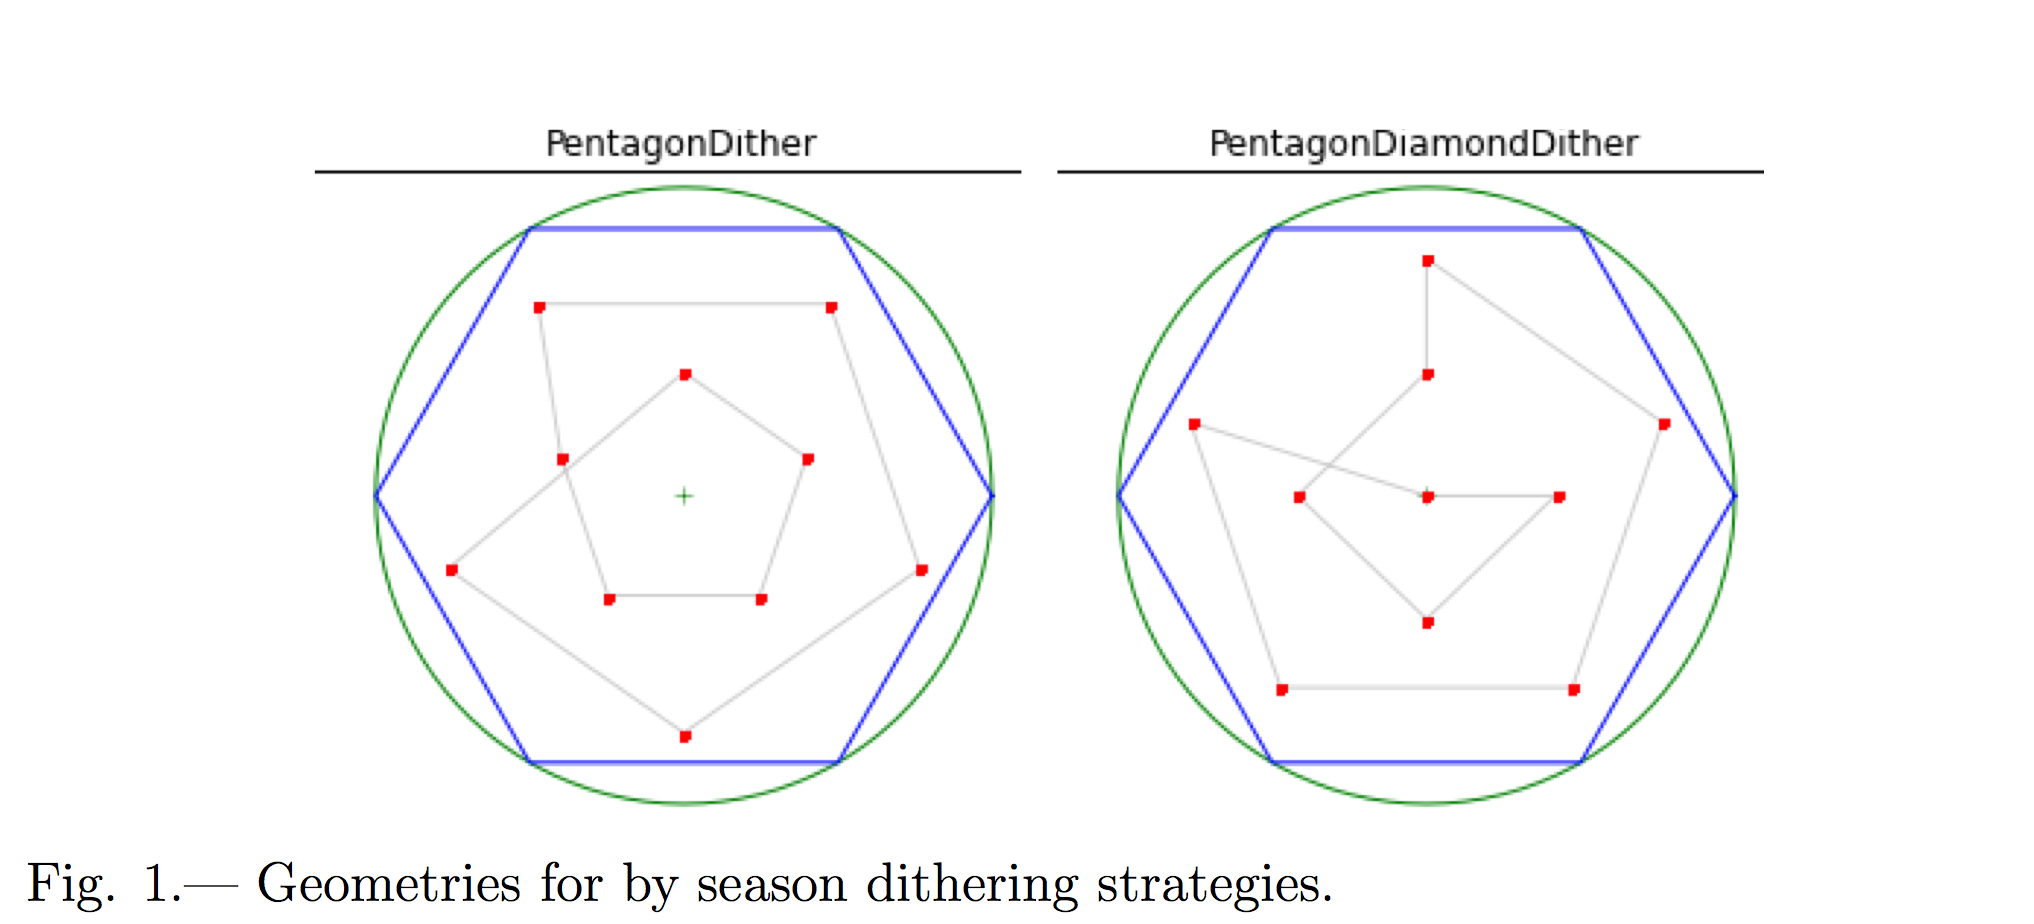
\includegraphics[angle=0,width=0.99\hsize:,clip]{figs/awan_fig1.png}
%\vskip -1.3in
\caption{}
\label{fig:seasonal_dithers}
\end{figure}
%%%%%%%%%%%%%%%%%%%%%%%%%%%%%%%%%

%%%%%%%%%%%%%%%%%%%%%%%%%%%%%%%%%
\begin{figure}[tbh!]
\vskip -0.1in
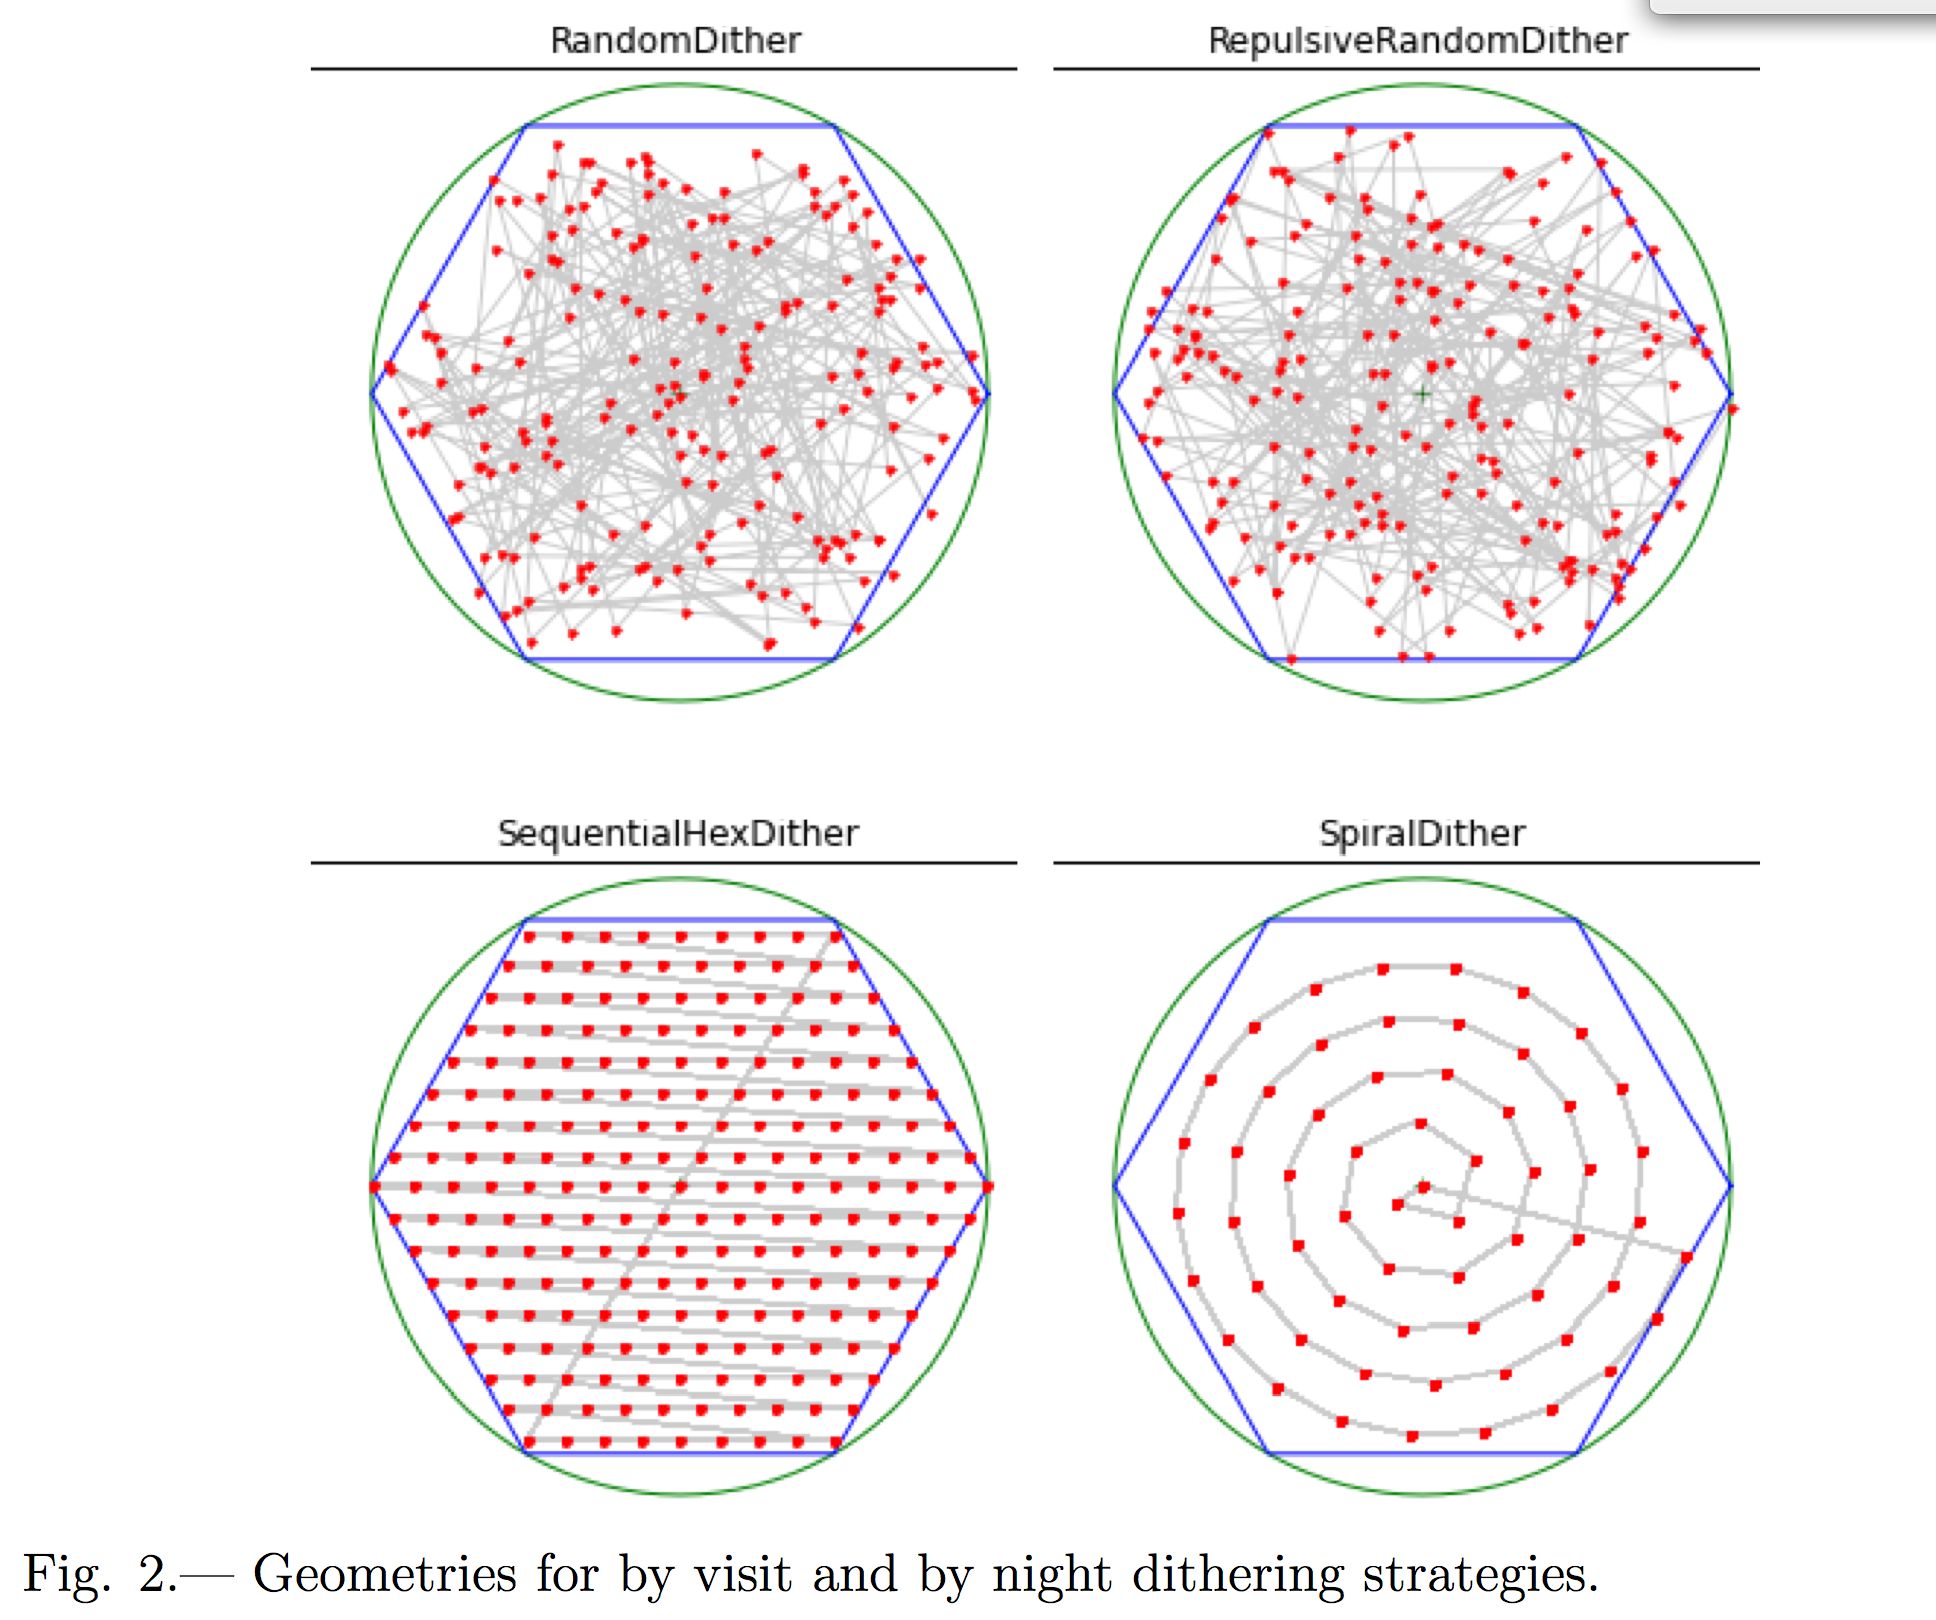
\includegraphics[angle=0,width=0.99\hsize:,clip]{figs/awan_fig2.png}
%\vskip -1.3in
\caption{}
\label{fig:nightly_dithers}
\end{figure}
%%%%%%%%%%%%%%%%%%%%%%%%%%%%%%%%%

%%%%%%%%%%%%%%%%%%%%%%%%%%%%%%%%%
\begin{figure}[tbh!]
\vskip -0.1in
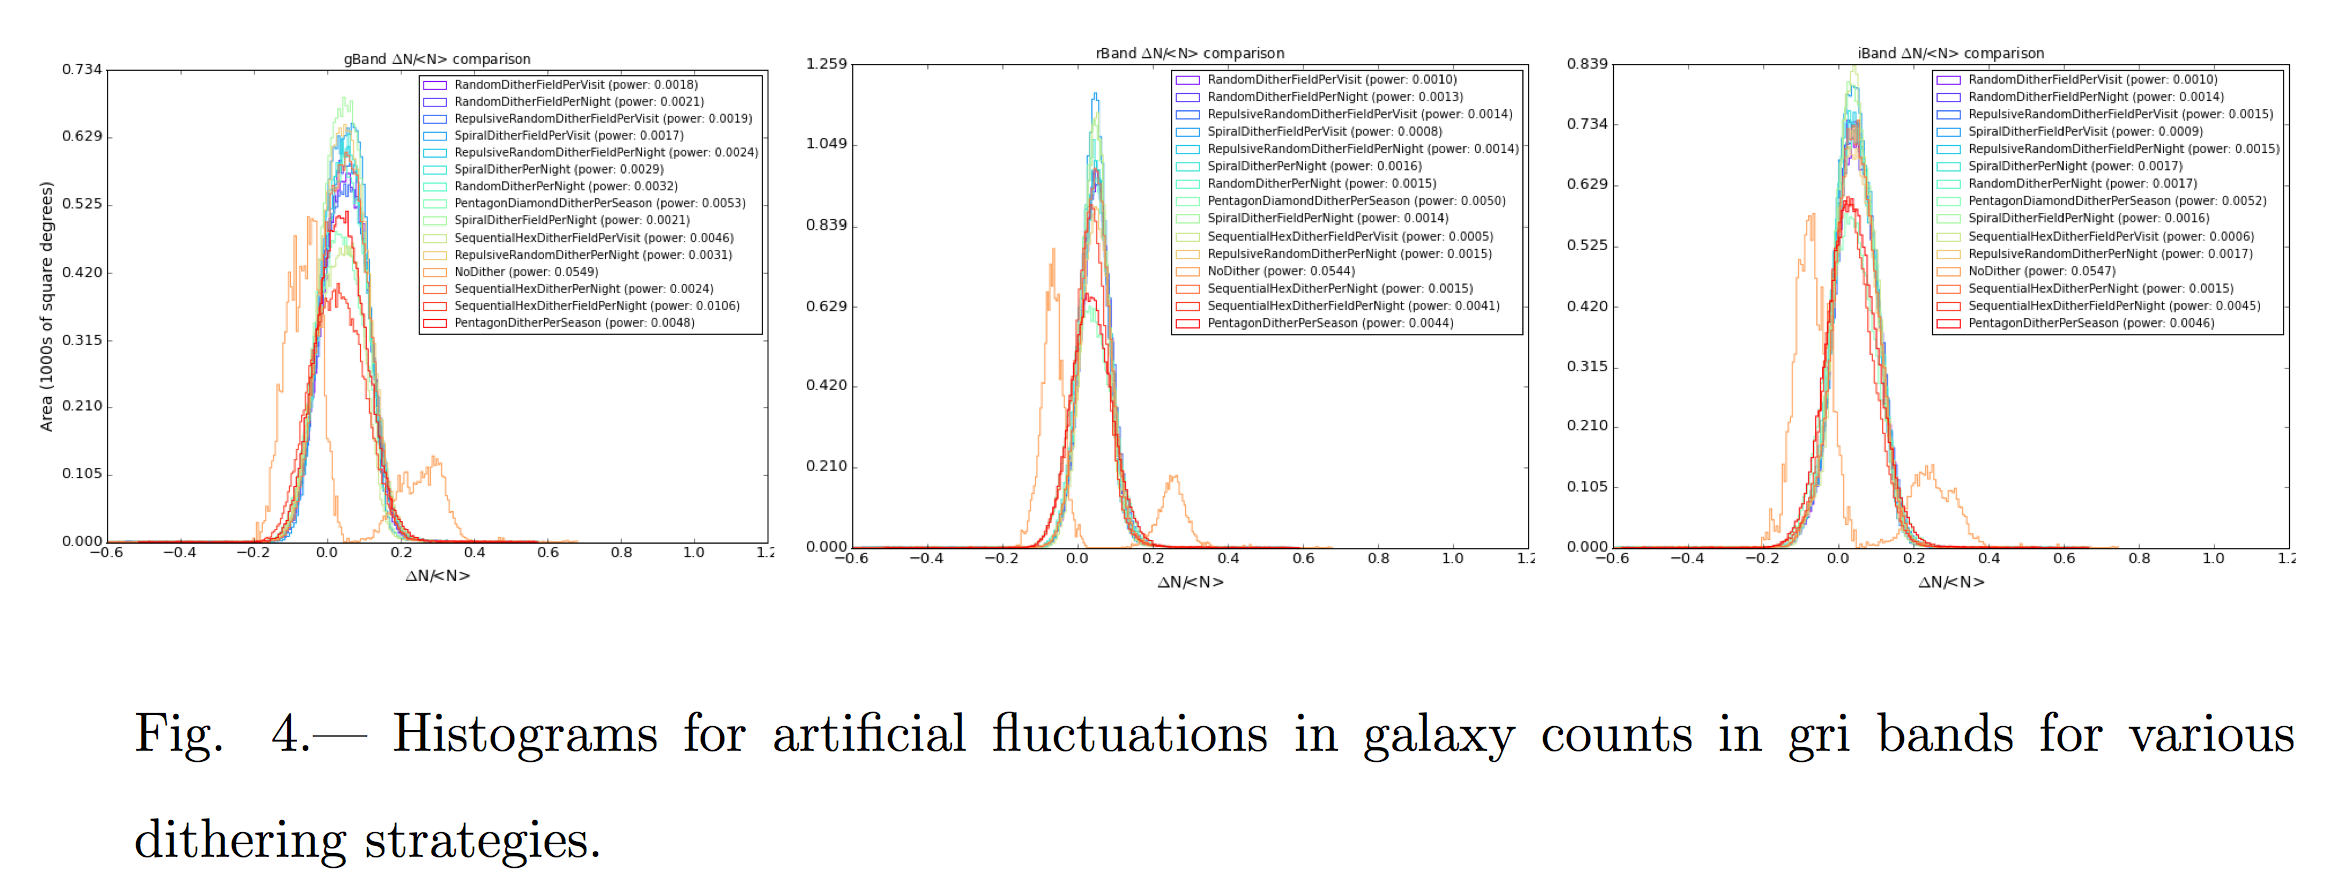
\includegraphics[angle=0,width=0.99\hsize:,clip]{figs/awan_fig4.png}
%\vskip -1.3in
\caption{}
\label{fig:dithering_histograms}
\end{figure}
%%%%%%%%%%%%%%%%%%%%%%%%%%%%%%%%%

%%%%%%%%%%%%%%%%%%%%%%%%%%%%%%%%%
\begin{figure}[tbh!]
\vskip -0.1in
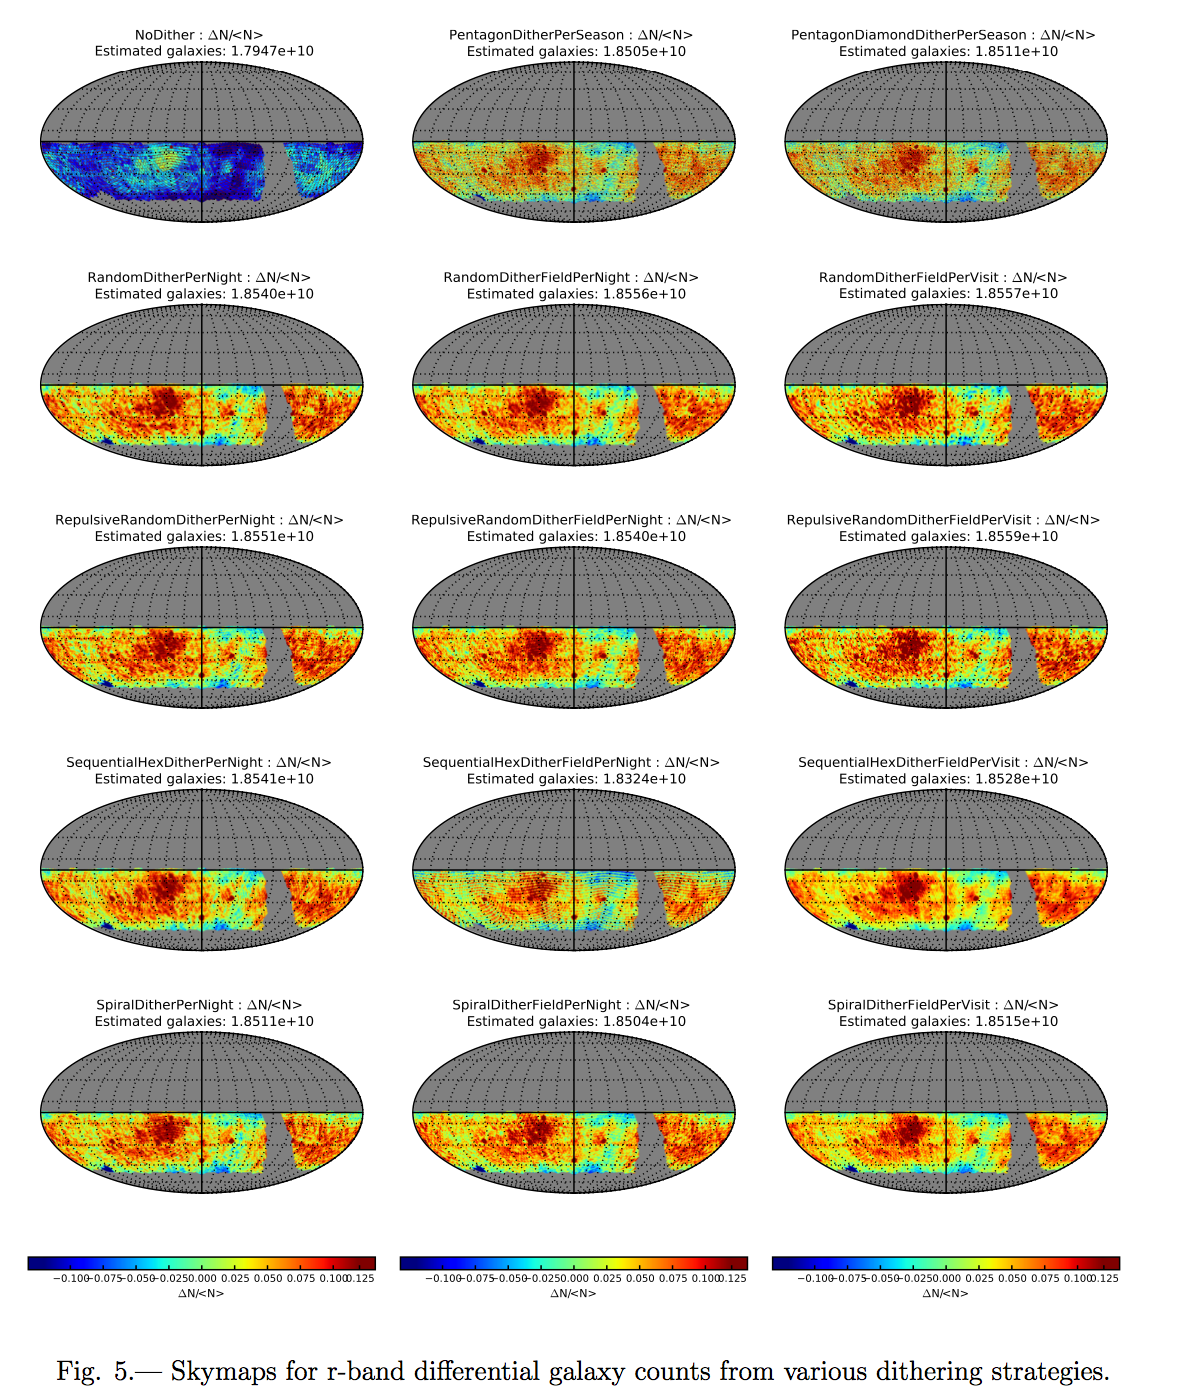
\includegraphics[angle=0,width=0.99\hsize:,clip]{figs/awan_fig5.png}
%\vskip -1.3in
\caption{}
\label{fig:dithering_skymaps}
\end{figure}
%%%%%%%%%%%%%%%%%%%%%%%%%%%%%%%%%

%%%%%%%%%%%%%%%%%%%%%%%%%%%%%%%%%
\begin{figure}[tbh!]
\vskip -0.1in
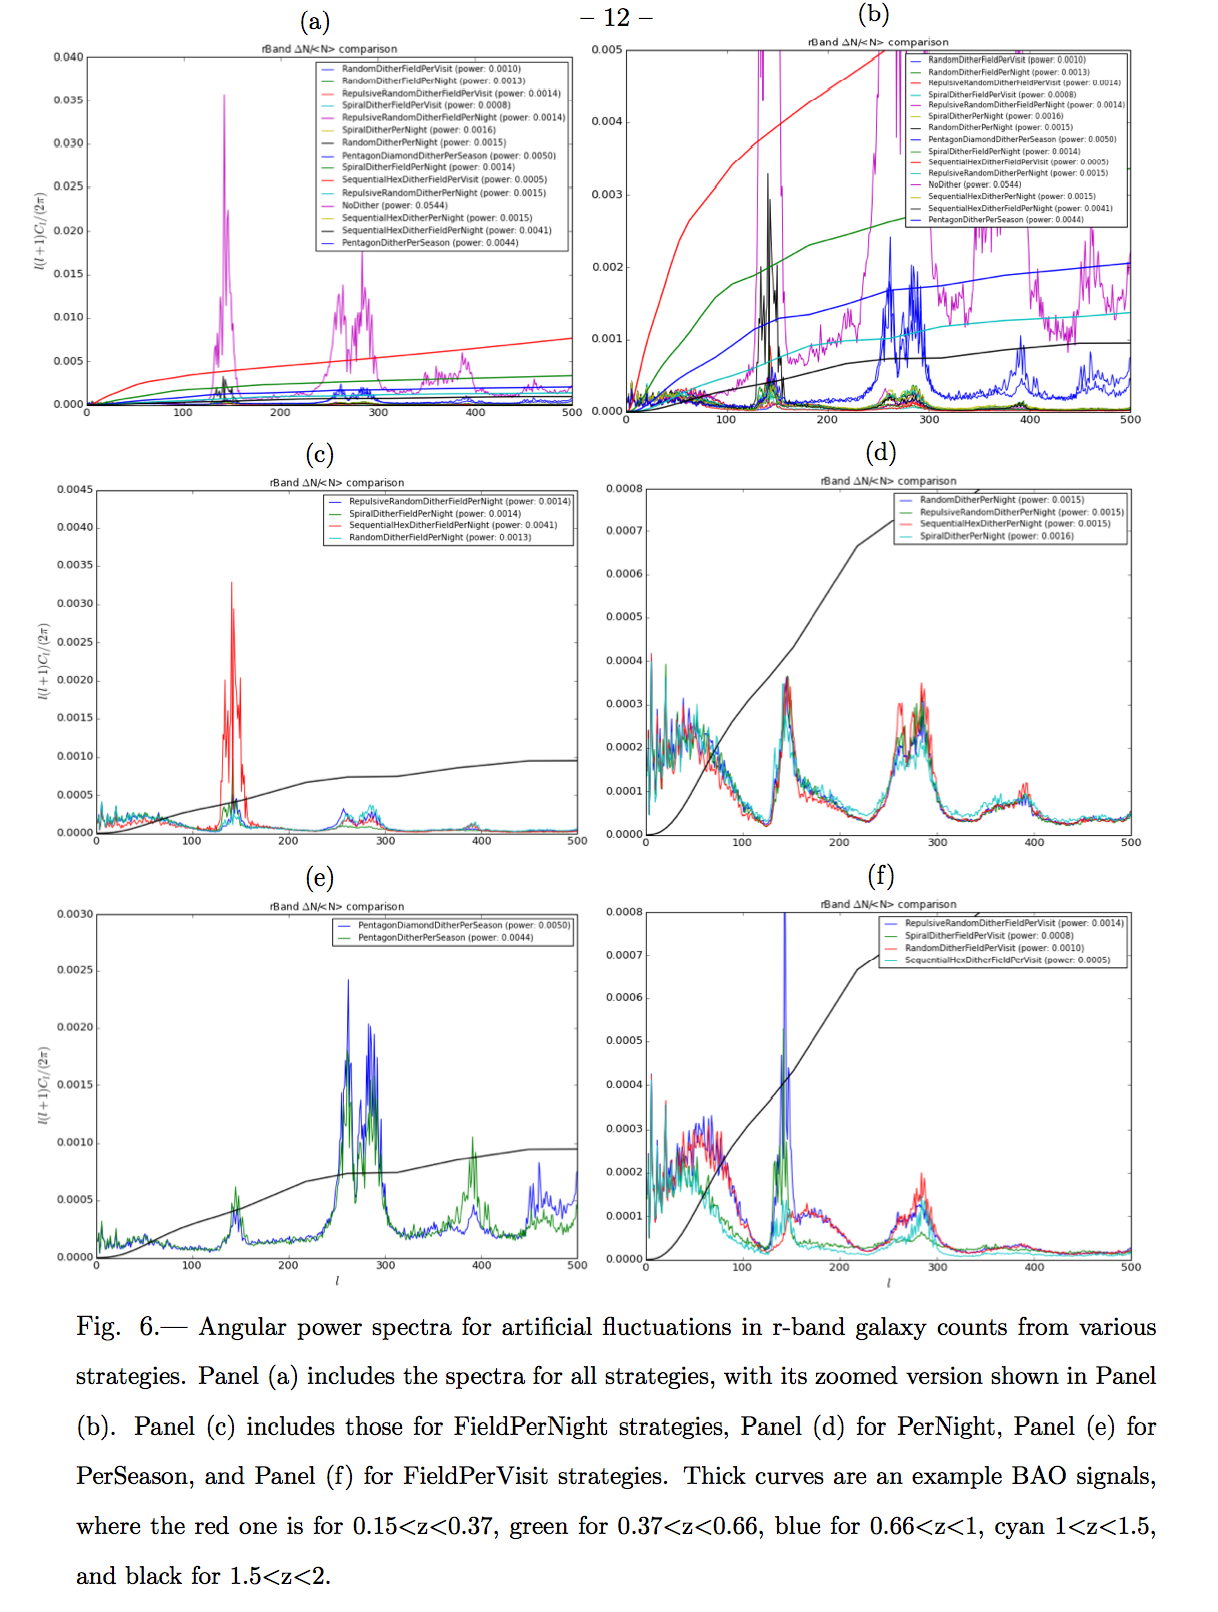
\includegraphics[angle=0,width=0.99\hsize:,clip]{figs/awan_fig6.png}
%\vskip -1.3in
\caption{}
\label{fig:dithering_power_spectra}
\end{figure}
%%%%%%%%%%%%%%%%%%%%%%%%%%%%%%%%%




%%%%%%%%%%%%%%%%%%%%%%%%%%%%%%%%%%%%
%\begin{figure*}[!ht]
%  \capstart
%  \begin{minipage}[b]{\linewidth}
%    \begin{minipage}[b]{0.32\linewidth}
%      \centering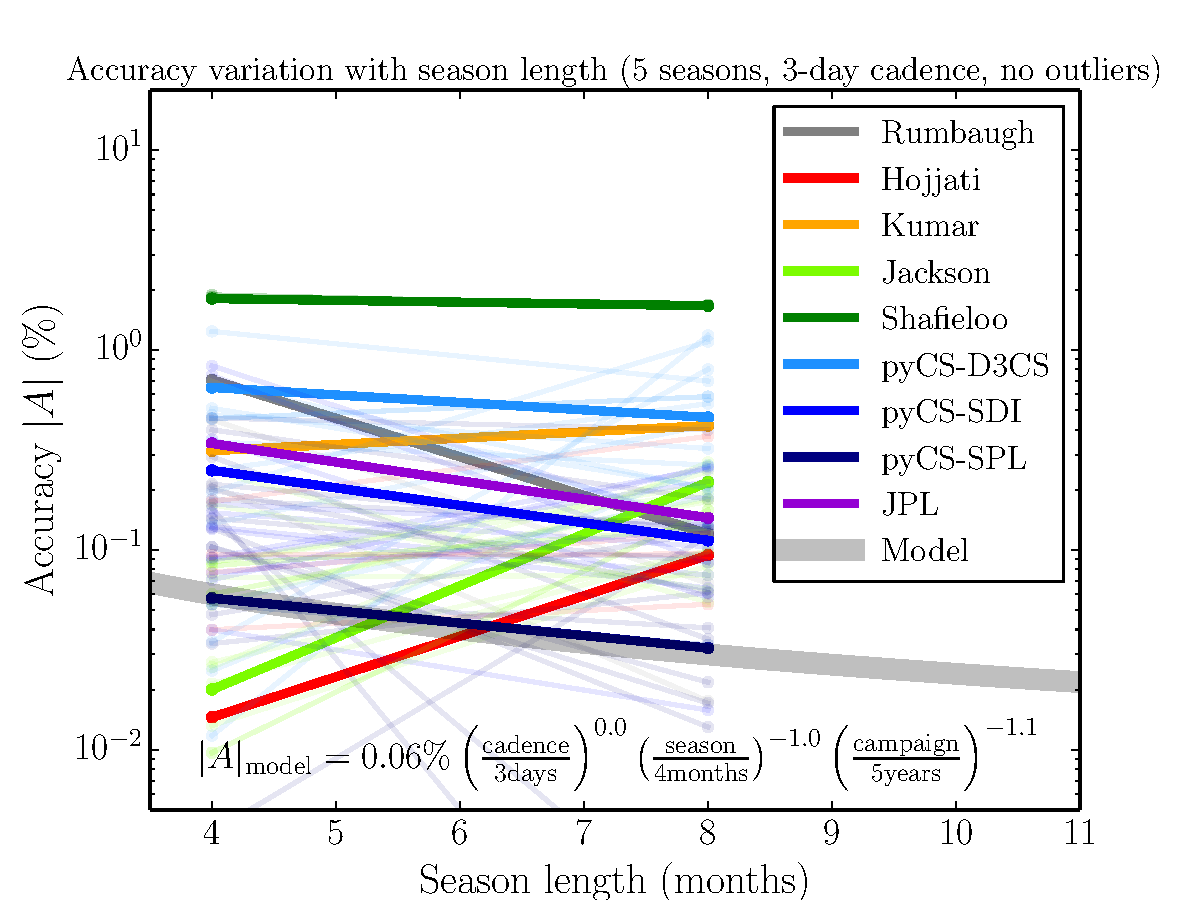
\includegraphics[width=\linewidth]{figs/Accuracy_season_nca.pdf}
%    \end{minipage} \hfill
%    \begin{minipage}[b]{0.32\linewidth}
%      \centering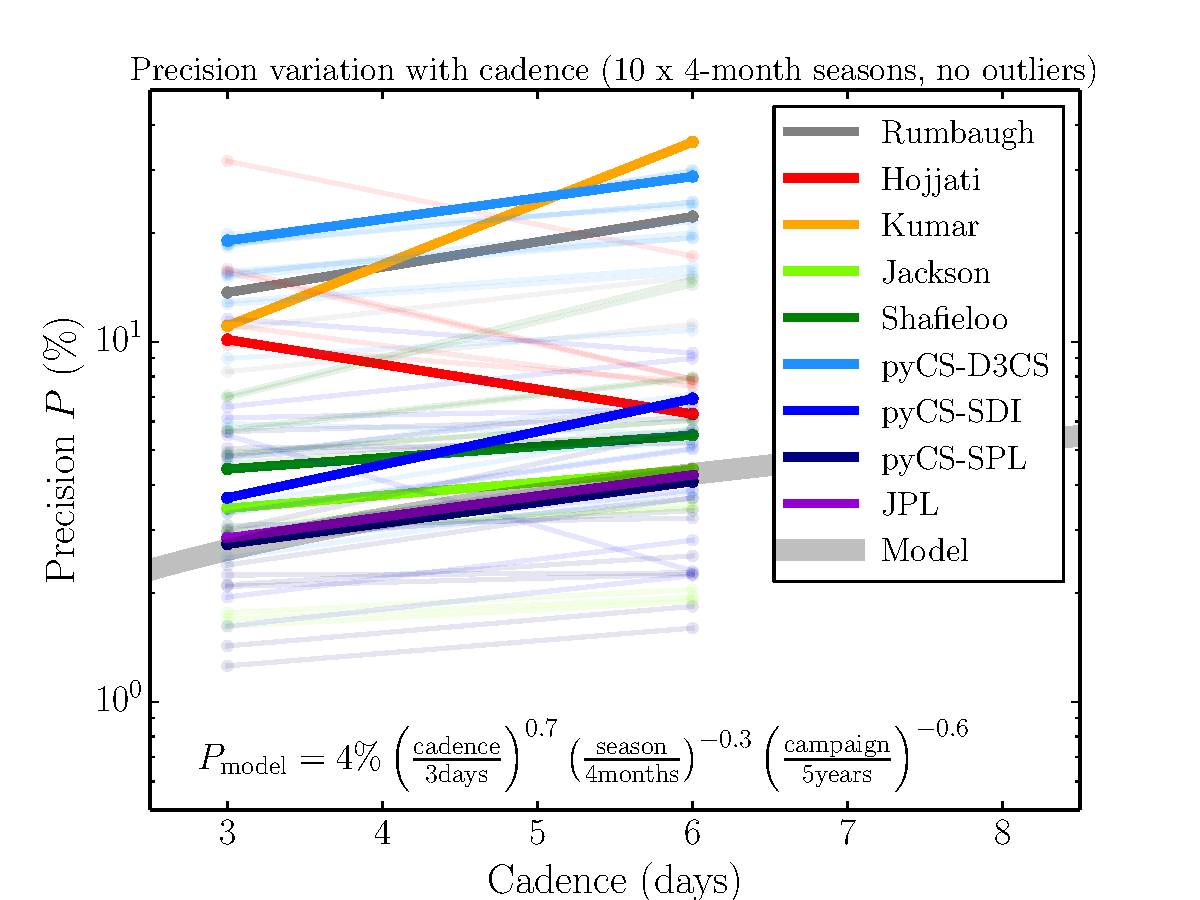
\includegraphics[width=\linewidth]{figs/Precision_cadence_nca.pdf}
%    \end{minipage} \hfill
%    \begin{minipage}[b]{0.32\linewidth}
%      \centering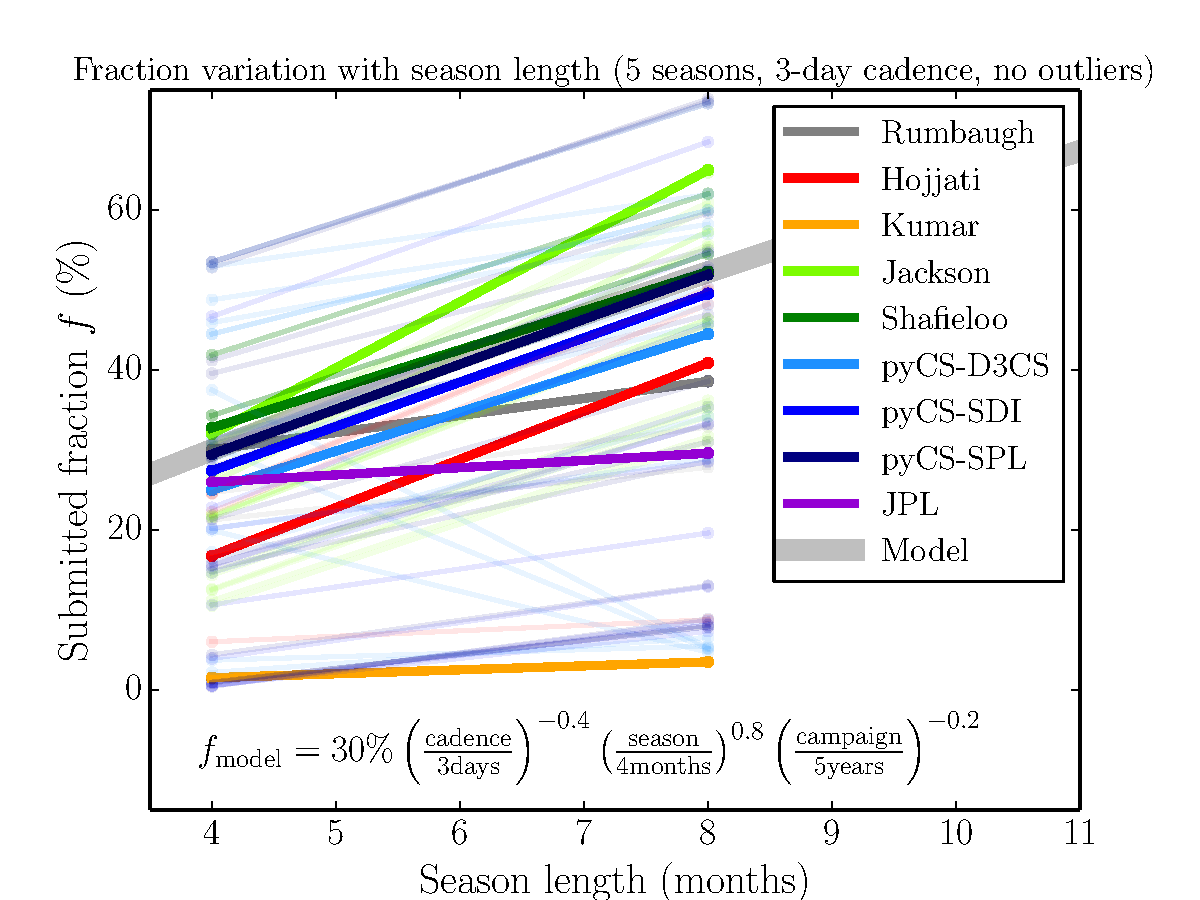
\includegraphics[width=\linewidth]{figs/Fraction_season_nca.pdf}
%    \end{minipage}
%  \end{minipage}
%\caption{Examples of changes in accuracy $A$ (left), precision $P$ (center) and success fraction $f$ (right) with schedule properties, as seen in the different TDC submissions. The gray
%approximate power law model was derived by visual inspection of the
%pyCS-SPL results; the signs of the indices were pre-determined according to our expectations. Reproduced from \citet{LiaoEtal2015}.}
%\label{fig:tdcresults}
%\end{figure*}
%%%%%%%%%%%%%%%%%%%%%%%%%%%%%%%%%%%


\todo{EG}{Input fuller results and text from Awan et al. draft.}  

%---------------------------------------------------------------------

\subsection{Discussion}
\label{sec:\secname:discussion}



\navigationbar

% ====================================================================
  

% --------------------------------------------------------------------

% ====================================================================
%+
% NAME:
%    lenstimedelays.tex
%
% ELEVATOR PITCH:
%    Lensed quasars and supernovae provide distance measurements for
%    cosmology. They are a few days to a few weeks in length. To
%    measure them well we need long campaigns (>~3 years) with high
%    night-to-night cadence (better than the standard 5 days if
%    possible, especially as combining all filters might be difficult.)
%
% COMMENTS:
%
%
% BUGS:
%
%
% AUTHORS:
%   Phil Marshall (@drphilmarshall)
%-
% ====================================================================

\section{ Strong Gravitational Lens Time Delays }
\label{sec:lenstimedelays}

\noindent{\it Phil Marshall} % (Writing team)

% This individual section will need to describe the particular
% discoveries and measurements that are being targeted in this section's
% science case. It will be helpful to think of a ``science case" as a
% ``science project" that the authors {\it actually plan to do}. Then,
% the sections can follow the tried and tested format of an observing
% proposal: a brief description of the investigation, with references,
% followed by a technical feasibility piece. This latter part will need
% to be quantified using the MAF framework, via a set of metrics that
% need to be computed for any given observing strategy to quantify its
% impact on the described science case. Ideally, these metrics would be
% combined in a well-motivated figure of merit. The section can conclude
% with a discussion of any risks that have been identified, and how
% these could be mitigated.

A short preamble goes here. What's the context for this science
project? Where does it fit in the big picture?

% --------------------------------------------------------------------

\subsection{Target measurements and discoveries}
\label{sec:lenstimedelays:targets}

Describe the discoveries and measurements you want to make.

Now, describe their response to the observing strategy. Qualitatively,
how will the science project be affected by the observing schedule and
conditions? In broad terms, how would we expect the observing strategy
to be optimized for this science?


% --------------------------------------------------------------------

\subsection{Metrics}
\label{sec:lenstimedelays:metrics}

Quantifying the response via MAF metrics: definition of the metrics,
and any derived overall figure of merit.


% --------------------------------------------------------------------

\subsection{OpSim Analysis}
\label{sec:lenstimedelays:analysis}

OpSim analysis: how good would the default observing strategy be, at
the time of writing for this science project?


% --------------------------------------------------------------------

\subsection{Discussion}
\label{sec:lenstimedelays:discussion}

Discussion: what risks have been identified? What suggestions could be
made to improve this science project's figure of merit, and mitigate
the identified risks?


% ====================================================================


% --------------------------------------------------------------------

% ====================================================================
%+
%
% SECTION NAME:
%    \secname.tex
%
% CHAPTER:
%    ???.tex
%
%
% COMMENTS:
%
%
% BUGS:
%
%
% AUTHORS:
%   Ohad Shemmer (@ohadshemmer), Timo Anguita (@tanguita), Niel Brandt, Gordon Richards, Scott Anderson(?),
%   Phil Marshall(?) (@drphilmarshall) 
%-
% ====================================================================

\section{AGN Science}
\def\secname{agn}\label{sec:\secname}

\noindent{\it Ohad Shemmer, Timo Anguita, Niel Brandt, Gordon Richards, Scott Anderson(?), Phil Marshall(?)}

% This section discusses the potential effects of the LSST observing strategy on AGN science. In short, there appears to be
% a consensus among the AGN and galaxies communities that AGN science will benefit from the most uniform cadence in
% terms of even sampling for each band and uniform sky coverage. It is also expected that any reasonable
% perturbation to the nominal LSST observing strategy will have mostly minor effects on AGN science. This section attempts
% to identify all the areas of AGN science that may be affected by the observing strategy and to point out the metrics that
% can be used to quantify any potential effect. Since the total number of metrics that must be quantified is quite large, and
% the effects are likely small in most cases, the goal of this section is to identify potential ``killers'' that may undermine
% key AGN research areas. For example, certain perturbations may reduce significantly the number of ``interesting'' AGNs,
% such as $z>6$ quasars, lensed quasars, or transient AGNs. Another example is photometric reverberation mapping
% which is one of LSST's greatest advantages for AGN research but is also very sensitive to the cadence; care must
% be taken to ensure that the observing strategy does not undermine the ability to make the best use of this method.

\subsection{AGN Selection and Census}
\label{sec:\secname:selection}

\noindent About $10^7 - 10^8$ AGNs will be selected in the main LSST survey using a combination of criteria, split
broadly into four categories: colors, astrometry, variability, and multiwavelength matching with other surveys.
The LSST observing strategy will affect mostly the first three of these categories.

{\bf Colors:}~The LSST observing strategy will determine the depth in each band, as a function of position on the sky, and will thus affect
the color selection of AGNs. This will eventually determine the AGN $L-z$ distribution and, in particular, may affect the identification
of quasars at $z\gtsim 6$ if, for example, $Y$-band exposures will not be sufficiently deep.

{\bf Variability:} AGNs can be effectively distinguished from (variable) stars, and from quiescent galaxies, by exhibiting certain characteristic variability patterns (e.g., Butler \& Bloom 2011). Non-uniform sampling may ``contaminate'' the variability signal of AGN candidates.

{\bf Astrometry:} AGNs will be selected among sources having zero proper motion, within the uncertainties. The LSST cadence
may affect the level of this uncertainty in each band, and may therefore affect the ability to identify (mostly fainter) AGNs.
%
Differential chromatic refraction (DCR), making use of the astrometric offset a source with emission lines has with respect to
a source with a featureless power-law spectrum, can help in the selection of AGNs and in confirming their photometric redshifts (Kaczmarczik~et~al.~2009). The DCR effect is more pronounced at higher airmasses. AGN selection and photometric redshift confirmation may be affected since the LSST cadence will affect the airmass distribution, in each band, for each AGN candidate.

\subsection{AGN Clustering}
\label{sec:\secname:clustering}

\noindent Measurements of the spatial clustering of AGNs with respect to those of quiescent galaxies can provide clues as to how galaxies
form inside their dark-matter halos and what causes the growth of their supermassive black holes (SMBHs). The impressive inventory 
of LSST AGNs will enable the clustering, and thus the host galaxy halo mass, to be determined over the widest range ranges of cosmic
epoch and accretion power.
%
The LSST cadence will not only affect the overall AGN census and its $L-z$ distribution, but also the
depth in each band as a function of sky position that can directly affect the clustering signal.

\subsection{AGNs and the Time Domain}
\label{sec:\secname:time}

{\bf AGN Variability:} A variety of AGN variability studies will be enabled by LSST. These are intended to probe the physical properties of the unresolved inner regions of the central engine. Relations will be sought between variability amplitude and timescale vs. $L$, $z$, $\lambda_{\rm eff}$, color, multiwavelength and spectroscopic properties, if available. The LSST sampling is expected to provide high-quality power spectral density functions for a large number of AGNs; these can be used to constrain the SMBH mass and accretion rate/mode. Furthermore, LSST AGNs exhibiting excess variability over that expected from their luminosities will be further scrutinized as candidates for lensed systems having unresolved images with the excess (extrinsic) variability being attributed mainly to microlensing.

Photometric reverberation mapping (PRM), measuring the time-delayed response of either the flux of the broad emission line region (BELR) lines to the flux of the AGN continuum or between the continuum flux in one (longer wavelength) band to the continuum flux in another (band with shorter wavelength), will be one of the cornerstones of AGN research in the LSST era
(e.g., Chelouche 2013; Chelouche \& Zucker 2013; Chelouche~et~al.~2014). For example, LSST is expected to deliver BELR line-continuum time delays in $\sim10^5-10^6$ sources, which is unprecedented when compared to $\sim50-100$ such measurements conducted via the traditional, yet much more expensive (per source) spectroscopic method. Sources in the deep-drilling fields (DDFs) will benefit from the highest quality PRM
time-delay measurements given the factor of $\sim10$ denser sampling. The PRM measurements will probe the size and structure of the accretion disk and BELR, in a statistical sense, and may provide improved SMBH mass estimates for sources that have at least single-epoch spectra.

The PRM method is very sensitive to the sampling in each band, therefore the ability to derive reliable time delays can be affected significantly
by the LSST cadence. The best results will be obtained by having the most uniform sampling equally for each band. Additionally, there is
a trade-off between the number of DDFs and the number of time delays that PRM can obtain (Chelouche~et~al.~2014). For example,
an increase in the number of DDFs, with similarly dense sampling in each field, can yield a proportionately larger number of high-quality time delays,
down to lower luminosities, but at the expense of far fewer time delays (of relatively high luminosity sources) in the main survey.

{\bf Time Delays in Gravitationally Lensed Quasars:} This aspect is discussed in detail in the lenstimedelays.tex section.

{\bf AGN Size and Structure with Microlensing:} Microlensing due to stars projected on top of individual lensed quasar images produce additional magnification. Using the fact that the Einstein radii of stars in lensing galaxies closely match the scales of different emission regions in high-redshift AGNs (micro-arcseconds), analyzing microlensing induced flux variations statistically on individual systems allows us to measure ``sizes'' of AGN regions.
%
Assuming a thermal profile for accretion disks, sizes in different emission wavelengths will be probed and as such, constraints on the slope of this thermal profile. Given the sheer number of lensed systems that LSST is expected to discover ($\sim8000$), this will allow us to stack systems for better constraints and hopefully determine the evolution of the size and profile. Due to the typical relative velocities of lenses, microlenses, observers (Earth) and source AGN, the microlensing variation timescales are between months to a few decades.

The quasar microlensing optical depth is $\sim1$, so every lensed quasar should be affected by microlensing at any given point in time. However, measurable variability can occur on longer timescales. Mosquera~et~al.~(2011) did a study using all known lensed quasars. They found the median timescale between high magnification events (Einstein crossing time scales) in the observed $I$-band is of the order of $\sim20$~yr (with a distribution between 10 and 40~yr). However, the source crossing time (duration of a high magnification event) is $\sim7.3$~months (with a distribution tail up to 3~yr). This basically means that out of all the lensed quasar {\em images} (microlensing between images is completely uncorrelated) about half of them will be quiescent during the 10~yr baseline of LSST. However, since the typical number of lensed images is either two or four, it means that, statistically, in every system, one (for doubles) or two (for quads) high magnification events should be observed in 10~yr of LSST monitoring.

Note that, the important cadence parameter is the source crossing time, as it is the length of the event to be as uniformly sampled as possible. The 7.3 months crossing time is the median for the observed $i$-band, but this time would be significantly shorter for bluer bands: for a thermal profile with slope $\alpha: R_\lambda \propto \lambda^\alpha$ implies source crossing time $t_{\rm s} \propto \lambda^{1/\alpha} \rightarrow t_u=t_i \times (\lambda_{\rm u} / \lambda_{\rm i})^{1/\alpha}$. For a Shakura-Sunyaev slope of $\alpha=0.75$ this would correspond to $7.3 \times (3600/8140)^{4/3}$ months $\approx 2.5$ months in the $u$-band.

In terms of the cadence, at least three evenly sampled data points per band within 2 to 3 months would be preferred to be able to map the constraining high magnification event(?). Hopefully uniformly spaced. Very tight cadence (e.g., DDFs) would increase the constraints significantly. However, since lensed quasars are not that common, this smaller area would mean only a few ($\sim80$?) suitable systems monitored in the DDFs.
%
Regarding the season length, the ``months'' timescale of high magnification events very likely means that we can/will miss high magnification events in the season gaps, at least in the bluer bands.
%
Killer: observations spread on timescales larger than 3 months(??). This would likely miss the high magnification events. In those cases we could perhaps consider close consecutive photometric bands as equivalent accretion disk regions, however this would mean weaker constraints on the thermal profile.
%
Important Note: all this science needs to be done on lensed quasars with measured or very short time delays to remove the intrinsic variability signal, which might significantly reduce the sample.

{\bf Microlensing Aided Reverberation Mapping:} Given that microlensing mostly affects continuum emission rather than BELR line emission, microlensing may enable disentangling the BELR line $+$ continuum emission in single photometric bands, allowing the use of single broad band PRM measurements (Sluse \& Tewes 2014). As with the two-band PRM method discussed above, the denser (and the longer) the sampling, the more accurate are the constraints that can be obtained for the time delays.

{\bf Transient AGN and TDEs:} This aspect is discussed in detail in the variablesandtransients.tex section(?)

% --------------------------------------------------------------------

\subsection{Metrics}
\label{sec:\secname:metrics}

% Quantifying the main impacts on AGN science via MAF metrics, including the effects
% of additional cadence facto,rs such as the number of DDFs
% and MC fields, or different dithering patterns,: definition of the metrics,
% and any derived overall figure of merit.

% --------------------------------------------------------------------

\subsection{Discussion}
\label{sec:\secname:discussion}

% Discussion: what risks have been identified? What suggestions could be
% made to improve the figures of merit, and mitigate the identified risks?
% What ``tweaks'', if any, can be proposed to the nominal LSST observing strategy
% in order to help achieve key AGN science goals?

\navigationbar


% --------------------------------------------------------------------

% ====================================================================
%+
% SECTION:
%    supernovacosmology.tex
%
% CHAPTER:
%    cosmology.tex
%
% ELEVATOR PITCH:
%    SNIa cosmology, approach to evaluating dependence of science on cadence
%
% COMMENTS:
%
%
% BUGS:
%
%
% AUTHORS:
%    Phil Marshall (@drphilmarshall)  - put your name and GitHub username here!
%-
% ====================================================================

\section{Supernova Cosmology and Physics}
\def\secname{supernovae}\label{sec:\secname}
% \label{sec:cosmology, supernovae, classification, lenstimedelays, deepdrillingfields }

\noindent{\it Jeonghee Rho, Michelle Lochner, Rahul Biswas} % (Writing team)

% This individual section will need to describe the particular
% discoveries and measurements that are being targeted in this section's
% science case. It will be helpful to think of a ``science case" as a
% ``science project" that the authors {\it actually plan to do}. Then,
% the sections can follow the tried and tested format of an observing
% proposal: a brief description of the investigation, with references,
% followed by a technical feasibility piece. This latter part will need
% to be quantified using the MAF framework, via a set of metrics that
% need to be computed for any given observing strategy to quantify its
% impact on the described science case. Ideally, these metrics would be
% combined in a well-motivated figure of merit. The section can conclude
% with a discussion of any risks that have been identified, and how
% these could be mitigated.

This section is concerned with the detection and characterization of supernovae (SNe)
over time with LSST and their various scientific applications.
The most important
application is the use of supernovae type Ia (SNIa) and potentially some core-collapse SN (like type IIP) to trace the recent expansion history of the universe,
and confront models of the physics driving the late time accelerated expansion
of the universe. 

This objective of SN cosmology follows (at least for SNIa) results from several
highly successful surveys; improvement in knowledge of SN cosmology could come from
substantially larger numbers of well-characterized SNe and potentially
useful redshift distributions of such detected SNe. In this sense, this
goal is not directly tied to the unprecedentedly large survey area of LSST.  
However, we shall argue that in practice, even this
goal would benefit from the spatial scale offered by the Wide Fast Deep
(WFD) component of the LSST survey. 

On the other hand, the WFD component of the LSST survey is potentially the 
first single survey to scan for SNe across the very large area of the
entire Southern sky.  SNe that are detected and well characterized by LSST will
probe the isotropy of the universe.  Peculiar velocities of 
SNe will probe the growth of structure.  In addition, this large sample
will enable further
sharpening of our understanding of the properties of the supernova population 
of different types. 
This last point is extremely important for SN cosmology goals:  The success of SNIa cosmology has always been based on the empirical model that intrinsic peak brightnesses are related to the certain observable characteristics of SNe. 
%While the spatial locations of the SNe are not important
The 
WFD has the potential to dramatically increase the size of the sample 
available to train such an empirical model, as well understand the probability of deviations and scatter from this model. Aside from issues like calibration 
which need to be addressed differently, a larger sample of such well measured SNe is probably the only way to address `systematics' due to deviations from the empirical
model. The anticipated sample can be thought of as consisting of two 
components:  the low-redshift sample which is more likely to be complete, and the higher-redshift sample that will be able to constrain evolution. 
% --------------------------------------------------------------------

\subsection{Target measurements and discoveries}
\label{sec:keyword:targets}

% Describe the discoveries and measurements you want to make.

SNe of different types are visible over time scales of about a few 
weeks (e.g., type Ia) to nearly a year (type IIP).  During the full ten-year
 survey, LSST will scan the entire southern sky repeatedly
 with a WFD cadence, and certain specific locations
of the sky called the Deep Drilling Fields (DDF) with special enhanced cadence. 

This spatio-temporal window should contain millions (RB: remember to check) of SNe, that will have apparent magnitudes brighter than the single exposure limiting magnitude of LSST.  However, the actual
 sequence of observations by LSST, defined by the series of field pointings as a
 function of time in filter bands (along with weather conditions) will
 determine the extent to which each SN can be detected and
 characterized well.  Characterization of the SNe is at the core of a
 number of science programs that use them as bright, abundant objects with empirically determined intrinsic brightness. For LSST, this goal entails (a) detection of SNe, (b) photometric typing of SNe, (c) estimating photometric redshifts of SNe (or identifying host galaxies 
 and obtaining their redshifts from photometry or follow-up spectroscopy),
(d) estimation of intrinsic brightnesses of the SNe, and finally use of these data in addressing our science goals of cosmological inference, etc.
The efficacy of photometric typing, redshifts and estimation of intrinsic brightnesses are all
dependent on the amount of information available in the observed light curves of SNe. While these steps are not necessarily independent, it is useful to think of the requirements on some of these steps separately; it is not unlikely  that combining some of these steps would still be affected by similar requirements. 

{\emph{Our first objective is to detect such SNe}}, by which we mean
selecting SNe from among the transient sources detected by LSST.
% classify them as SNe (as opposed to an AGN, or an asteroid). 
In brief, this process 
consists of defining a set of image subtractions between high 
resolution `template` image of a sky section, and a set of single exposures at
different times (usually of lower resolution) of the same region, after 
accounting for the different resolutions of images, and alignments. These sets of image subtractions associated
 with a single object will be used to detect the object as a transient and then
classify the transient as an SN. Clearly, detecting an SN depends on the number of such images recorded per object, the number of filters, and the signal-to-noise ratios of the images. %One might expect that 
The efficiency of this step may be summarized as a threshold on the joint properties 
of an astrophysical candidate (apparent brightness, light curve characteristics, background) as well as observing conditions (astronomical seeing, etc.).  

{\emph{Our second objective is to photometrically classify different kinds of SNe.}} 
%{\bfseries Photometric SN classification}\\
Previously, only spectroscopically typed SNe have been used for cosmology. Photometric 
typing from light curves alone has only been used to select candidates for spectroscopic 
follow-up (see, e.g., \citet{Sako2008}). However, LSST will simply find far too many 
candidates for even a significant fraction of them to be followed up spectroscopically. In order to avoid 
discarding the majority of the SN dataset, we need to use techniques capable of 
determining cosmological parameters from a potentially contaminated photometric SN dataset.

Several techniques have been proposed in recently to solve this problem. One 
approach proposes applying stringent cuts to the photometric dataset to obtain a nearly pure sample 
of SNIa\citep{Bernstein2012,Campbell2013} and to run the standard SNIa cosmology analysis 
with this sample. Another approach, BEAMS \citep{Kunz2007,Newling2011,Hlozek2012,Knights2013}, 
makes use of an entire dataset, coping with contamination by using a mixture model for the 
likelihood, thus allowing for multiple populations. Whatever the technique ultimately used for 
cosmological analysis, it will rely on accurate initial classifications of SN type and 
unbiased estimates for the probability of each type.

Current state-of-the-art photometric classification techniques rely on fitting empirically 
determined templates of SNe to light curves \citep{Jha2007,Guy2007,Sako2011}. However in 
recent years, new approaches have been developed in response to the 2010 `Supernova 
Photometric Classification Challenge' \citep{Kessler2010a}. Many of these use novel light curve 
parameterization and employ machine learning algorithms to perform the classification (see \citet{Kessler2010b} and references therein).

While many of these methods have been tested on standard sets of simulated data and (in some cases) 
on SDSS data, which technique (if any) is superior in all situations is unclear. For 
example, some techniques are dependent on the availability of reliable redshift information. 
%, while others  are less reliant on it. 
Some techniques may be more robust to non-representative datasets [Not sure what this means] than 
others, and how the techniques will respond to changes in cadence, filter sets, signal-to-noise, 
etc., is unclear.  

With this in mind, we propose the use of a multifaceted classification system which employs 
several different methods for extracting features from the light curves (e.g., fitting parametric 
functions or templates) and several different classification algorithms. This system is highly 
modular, allowing new approaches for direct comparison with existing  techniques to be added easily. This also allows direct analysis of different observing strategies, without requiring 
an initial choice of classification technique. 


{\emph{Our third objective is to characterize SNe in terms of empirical
    light curve models.}}

The ultimate goal of using SNe (type SNIa or SNIIP) for cosmology requires estimating their intrinsic brightnesses of the supernova. The
first (and sometimes only, depending on the light curve model) step is
fitting the calibrated fluxes to a light curve model with a set of parameters.
According to the ansatz used in SN cosmology, the intrinsic brightness of
 SNe is largely determined by the parameters of the light curve model; 
 hence the uncertainties on the inferred parameters largely determine the
 uncertainties on the inferred peak intrinsic brightness or distance moduli of the SNe.

% Now, describe their response to the observing strategy. Qualitatively,
% how will the science project be affected by the observing schedule and
% conditions? 

% In broad terms, how would we expect the observing strategy
% to be optimized for this science?





% --------------------------------------------------------------------

\subsection{Metrics}
\label{sec:keyword:metrics}

Quantifying the response via MAF metrics: definition of the metrics,
and any derived overall figure of merit.

\emph{To be added: discussion of the ROC curve as a useful metric for photometric supernova 
classification}




% --------------------------------------------------------------------

\subsection{OpsSim Analysis}
\label{sec:keyword:analysis}

OpSim analysis: how good would the default observing strategy be, at
the time of writing for this science project?

As noted above the scientific goal of characterizing SNe is to a large extent
dependent on how well the light curves of individual SNe are sampled in
time and filters. To study this, we re-index the OpsSim output on spatial
locations rather than use the temporal index. There are different methods (which will be merged), and here we will first illustrate this in terms the cadence in an example LSST field.

\begin{figure}
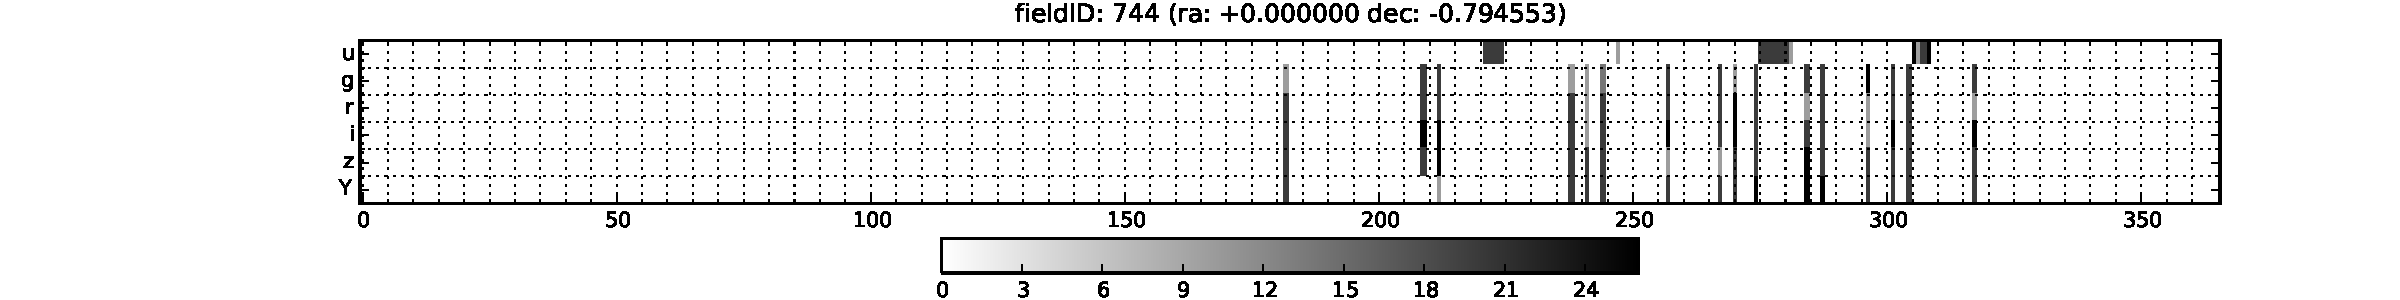
\includegraphics[width=\textwidth]{figs/supernova/fig_firstSeason_0}
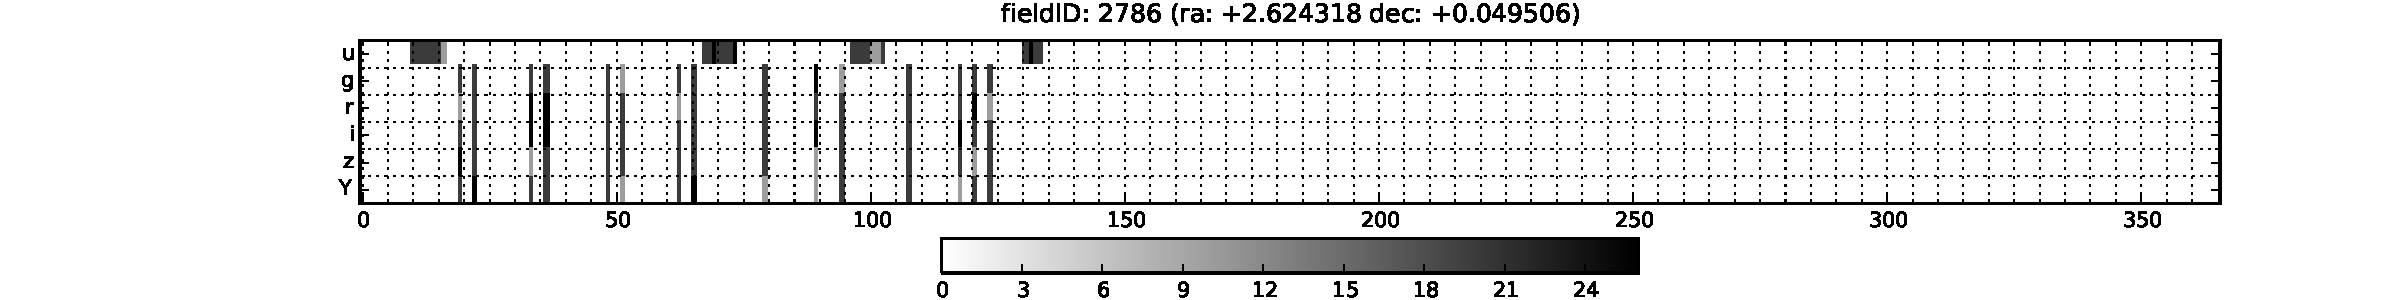
\includegraphics[width=\textwidth]{figs/supernova/fig_firstSeason_1}
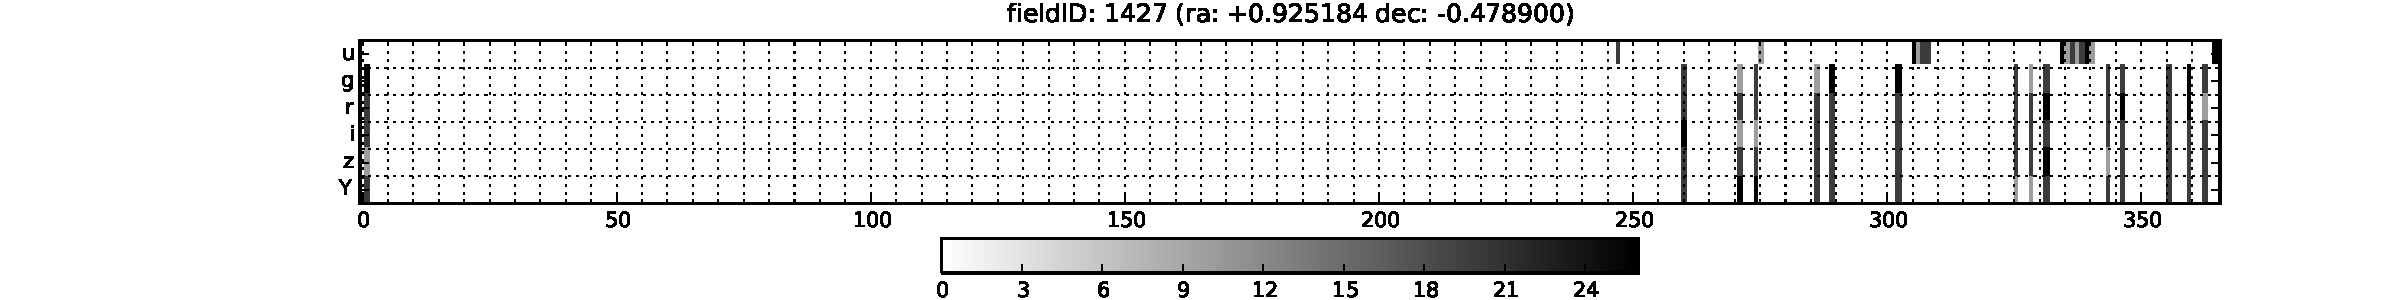
\includegraphics[width=\textwidth]{figs/supernova/fig_firstSeason_2}
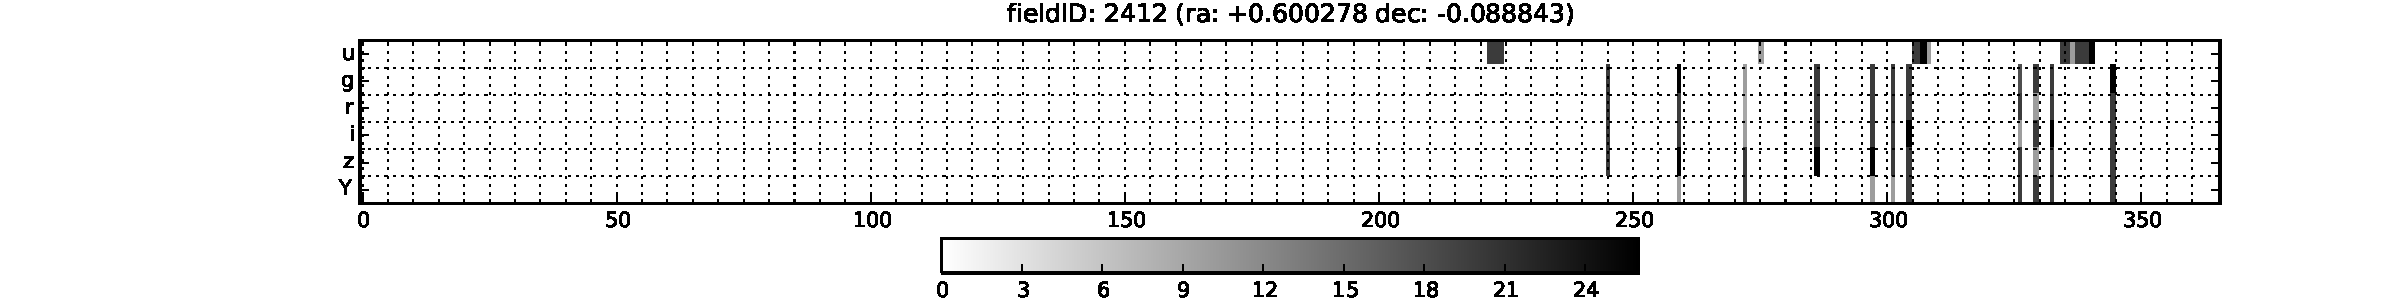
\includegraphics[width=\textwidth]{figs/supernova/fig_firstSeason_3}
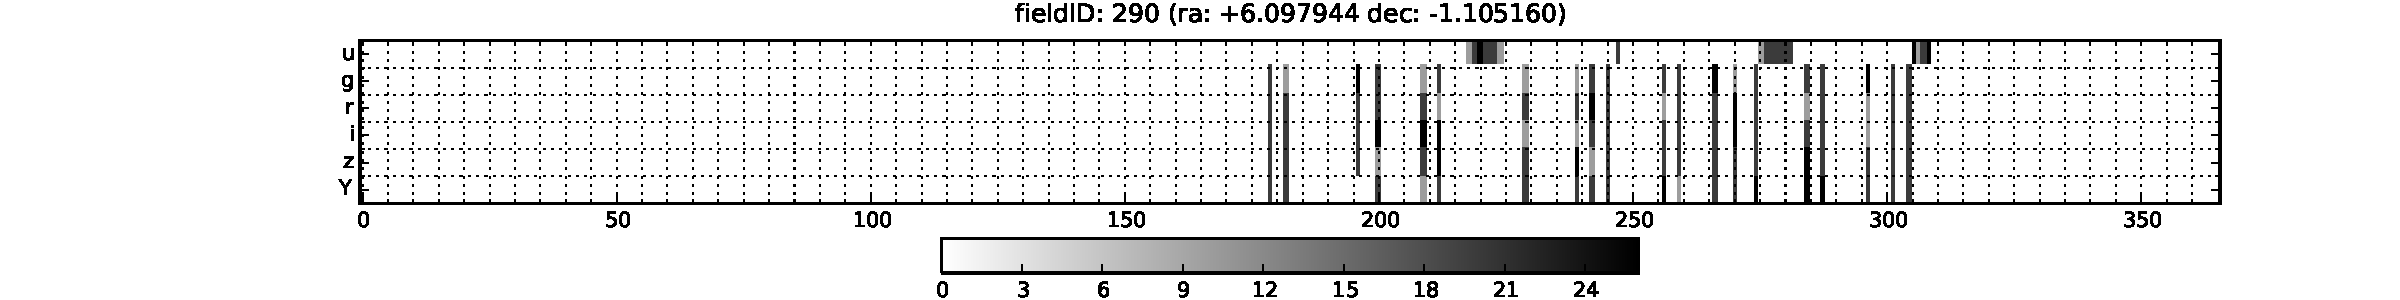
\includegraphics[width=\textwidth]{figs/supernova/fig_firstSeason_4}
\label{fig:opsimSummary}
\caption{Cadence in different filters for a few LSST DDFs in
    the the ouptut of OpSim version Enigma 1189. This ignores issues of chip 
gaps and overlaps between LSST pointings. These issues have been addressed in \citep{CarrollEtal2014} and Awan et.al. (2015, in prep.). We will add these to this analysis.}
\end{figure}



% --------------------------------------------------------------------

\subsection{Discussion}
\label{sec:keyword:discussion}

Discussion: what risks have been identified? What suggestions could be
made to improve this science project's figure of merit, and mitigate
the identified risks?


\begin{itemize}
\item Intrinsic Dispersion, environmental effects, newer analysis methods
\item Follow-up procedures: What is feasible? Where will our training samples for classification and light curve models come from (other experiments, our own 
sub-samples with spectroscopic follow-up?), spectroscopic follow-up of host galaxies. Can hosts be identified?
\item `Systematics': In what ways will the real data not match the assumptions made in analysis. Having a large sample of SN, to understand the astrophysics would be useful for this. 
\end{itemize}


% ====================================================================

\navigationbar


% --------------------------------------------------------------------


% --------------------------------------------------------------------

% ====================================================================
%+
% SECTION:
%    supernovacosmology.tex
%
% CHAPTER:
%    cosmology.tex
%
% ELEVATOR PITCH:
%    SNIa cosmology, approach to evaluating dependence of science on cadence
%
% COMMENTS:
%
%
% BUGS:
%
%
% AUTHORS:
%    Phil Marshall (@drphilmarshall)  - put your name and GitHub username here!
%-
% ====================================================================

\section{Supernova Cosmology and Physics}
\def\secname{supernovae}\label{sec:\secname}
% \label{sec:cosmology, supernovae, classification, lenstimedelays, deepdrillingfields }

\noindent{\it Jeonghee Rho, Michelle Lochner, Rahul Biswas} % (Writing team)

% This individual section will need to describe the particular
% discoveries and measurements that are being targeted in this section's
% science case. It will be helpful to think of a ``science case" as a
% ``science project" that the authors {\it actually plan to do}. Then,
% the sections can follow the tried and tested format of an observing
% proposal: a brief description of the investigation, with references,
% followed by a technical feasibility piece. This latter part will need
% to be quantified using the MAF framework, via a set of metrics that
% need to be computed for any given observing strategy to quantify its
% impact on the described science case. Ideally, these metrics would be
% combined in a well-motivated figure of merit. The section can conclude
% with a discussion of any risks that have been identified, and how
% these could be mitigated.

This section is concerned with the detection and characterization of supernovae (SNe)
over time with LSST and their various scientific applications.
The most important
application is the use of supernovae type Ia (SNIa) and potentially some core-collapse SN (like type IIP) to trace the recent expansion history of the universe,
and confront models of the physics driving the late time accelerated expansion
of the universe. 

This objective of SN cosmology follows (at least for SNIa) results from several
highly successful surveys; improvement in knowledge of SN cosmology could come from
substantially larger numbers of well-characterized SNe and potentially
useful redshift distributions of such detected SNe. In this sense, this
goal is not directly tied to the unprecedentedly large survey area of LSST.  
However, we shall argue that in practice, even this
goal would benefit from the spatial scale offered by the Wide Fast Deep
(WFD) component of the LSST survey. 

On the other hand, the WFD component of the LSST survey is potentially the 
first single survey to scan for SNe across the very large area of the
entire Southern sky.  SNe that are detected and well characterized by LSST will
probe the isotropy of the universe.  Peculiar velocities of 
SNe will probe the growth of structure.  In addition, this large sample
will enable further
sharpening of our understanding of the properties of the supernova population 
of different types. 
This last point is extremely important for SN cosmology goals:  The success of SNIa cosmology has always been based on the empirical model that intrinsic peak brightnesses are related to the certain observable characteristics of SNe. 
%While the spatial locations of the SNe are not important
The 
WFD has the potential to dramatically increase the size of the sample 
available to train such an empirical model, as well understand the probability of deviations and scatter from this model. Aside from issues like calibration 
which need to be addressed differently, a larger sample of such well measured SNe is probably the only way to address `systematics' due to deviations from the empirical
model. The anticipated sample can be thought of as consisting of two 
components:  the low-redshift sample which is more likely to be complete, and the higher-redshift sample that will be able to constrain evolution. 
% --------------------------------------------------------------------

\subsection{Target measurements and discoveries}
\label{sec:keyword:targets}

% Describe the discoveries and measurements you want to make.

SNe of different types are visible over time scales of about a few 
weeks (e.g., type Ia) to nearly a year (type IIP).  During the full ten-year
 survey, LSST will scan the entire southern sky repeatedly
 with a WFD cadence, and certain specific locations
of the sky called the Deep Drilling Fields (DDF) with special enhanced cadence. 

This spatio-temporal window should contain millions (RB: remember to check) of SNe, that will have apparent magnitudes brighter than the single exposure limiting magnitude of LSST.  However, the actual
 sequence of observations by LSST, defined by the series of field pointings as a
 function of time in filter bands (along with weather conditions) will
 determine the extent to which each SN can be detected and
 characterized well.  Characterization of the SNe is at the core of a
 number of science programs that use them as bright, abundant objects with empirically determined intrinsic brightness. For LSST, this goal entails (a) detection of SNe, (b) photometric typing of SNe, (c) estimating photometric redshifts of SNe (or identifying host galaxies 
 and obtaining their redshifts from photometry or follow-up spectroscopy),
(d) estimation of intrinsic brightnesses of the SNe, and finally use of these data in addressing our science goals of cosmological inference, etc.
The efficacy of photometric typing, redshifts and estimation of intrinsic brightnesses are all
dependent on the amount of information available in the observed light curves of SNe. While these steps are not necessarily independent, it is useful to think of the requirements on some of these steps separately; it is not unlikely  that combining some of these steps would still be affected by similar requirements. 

{\emph{Our first objective is to detect such SNe}}, by which we mean
selecting SNe from among the transient sources detected by LSST.
% classify them as SNe (as opposed to an AGN, or an asteroid). 
In brief, this process 
consists of defining a set of image subtractions between high 
resolution `template` image of a sky section, and a set of single exposures at
different times (usually of lower resolution) of the same region, after 
accounting for the different resolutions of images, and alignments. These sets of image subtractions associated
 with a single object will be used to detect the object as a transient and then
classify the transient as an SN. Clearly, detecting an SN depends on the number of such images recorded per object, the number of filters, and the signal-to-noise ratios of the images. %One might expect that 
The efficiency of this step may be summarized as a threshold on the joint properties 
of an astrophysical candidate (apparent brightness, light curve characteristics, background) as well as observing conditions (astronomical seeing, etc.).  

{\emph{Our second objective is to photometrically classify different kinds of SNe.}} 
%{\bfseries Photometric SN classification}\\
Previously, only spectroscopically typed SNe have been used for cosmology. Photometric 
typing from light curves alone has only been used to select candidates for spectroscopic 
follow-up (see, e.g., \citet{Sako2008}). However, LSST will simply find far too many 
candidates for even a significant fraction of them to be followed up spectroscopically. In order to avoid 
discarding the majority of the SN dataset, we need to use techniques capable of 
determining cosmological parameters from a potentially contaminated photometric SN dataset.

Several techniques have been proposed in recently to solve this problem. One 
approach proposes applying stringent cuts to the photometric dataset to obtain a nearly pure sample 
of SNIa\citep{Bernstein2012,Campbell2013} and to run the standard SNIa cosmology analysis 
with this sample. Another approach, BEAMS \citep{Kunz2007,Newling2011,Hlozek2012,Knights2013}, 
makes use of an entire dataset, coping with contamination by using a mixture model for the 
likelihood, thus allowing for multiple populations. Whatever the technique ultimately used for 
cosmological analysis, it will rely on accurate initial classifications of SN type and 
unbiased estimates for the probability of each type.

Current state-of-the-art photometric classification techniques rely on fitting empirically 
determined templates of SNe to light curves \citep{Jha2007,Guy2007,Sako2011}. However in 
recent years, new approaches have been developed in response to the 2010 `Supernova 
Photometric Classification Challenge' \citep{Kessler2010a}. Many of these use novel light curve 
parameterization and employ machine learning algorithms to perform the classification (see \citet{Kessler2010b} and references therein).

While many of these methods have been tested on standard sets of simulated data and (in some cases) 
on SDSS data, which technique (if any) is superior in all situations is unclear. For 
example, some techniques are dependent on the availability of reliable redshift information. 
%, while others  are less reliant on it. 
Some techniques may be more robust to non-representative datasets [Not sure what this means] than 
others, and how the techniques will respond to changes in cadence, filter sets, signal-to-noise, 
etc., is unclear.  

With this in mind, we propose the use of a multifaceted classification system which employs 
several different methods for extracting features from the light curves (e.g., fitting parametric 
functions or templates) and several different classification algorithms. This system is highly 
modular, allowing new approaches for direct comparison with existing  techniques to be added easily. This also allows direct analysis of different observing strategies, without requiring 
an initial choice of classification technique. 


{\emph{Our third objective is to characterize SNe in terms of empirical
    light curve models.}}

The ultimate goal of using SNe (type SNIa or SNIIP) for cosmology requires estimating their intrinsic brightnesses of the supernova. The
first (and sometimes only, depending on the light curve model) step is
fitting the calibrated fluxes to a light curve model with a set of parameters.
According to the ansatz used in SN cosmology, the intrinsic brightness of
 SNe is largely determined by the parameters of the light curve model; 
 hence the uncertainties on the inferred parameters largely determine the
 uncertainties on the inferred peak intrinsic brightness or distance moduli of the SNe.

% Now, describe their response to the observing strategy. Qualitatively,
% how will the science project be affected by the observing schedule and
% conditions? 

% In broad terms, how would we expect the observing strategy
% to be optimized for this science?





% --------------------------------------------------------------------

\subsection{Metrics}
\label{sec:keyword:metrics}

Quantifying the response via MAF metrics: definition of the metrics,
and any derived overall figure of merit.

\emph{To be added: discussion of the ROC curve as a useful metric for photometric supernova 
classification}




% --------------------------------------------------------------------

\subsection{OpsSim Analysis}
\label{sec:keyword:analysis}

OpSim analysis: how good would the default observing strategy be, at
the time of writing for this science project?

As noted above the scientific goal of characterizing SNe is to a large extent
dependent on how well the light curves of individual SNe are sampled in
time and filters. To study this, we re-index the OpsSim output on spatial
locations rather than use the temporal index. There are different methods (which will be merged), and here we will first illustrate this in terms the cadence in an example LSST field.

\begin{figure}
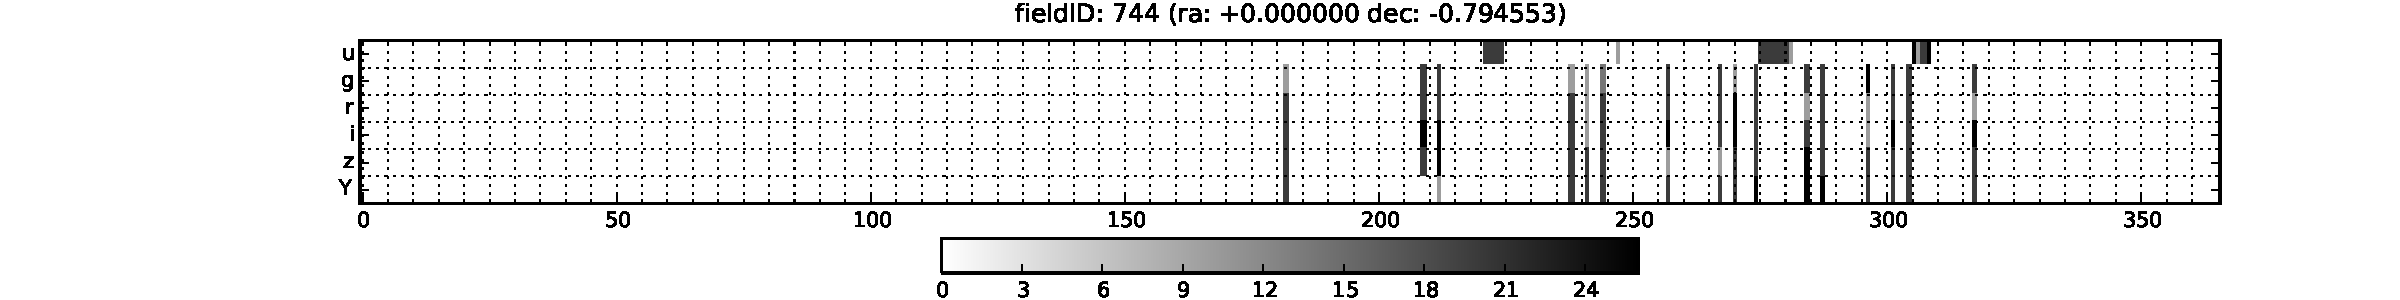
\includegraphics[width=\textwidth]{figs/supernova/fig_firstSeason_0}
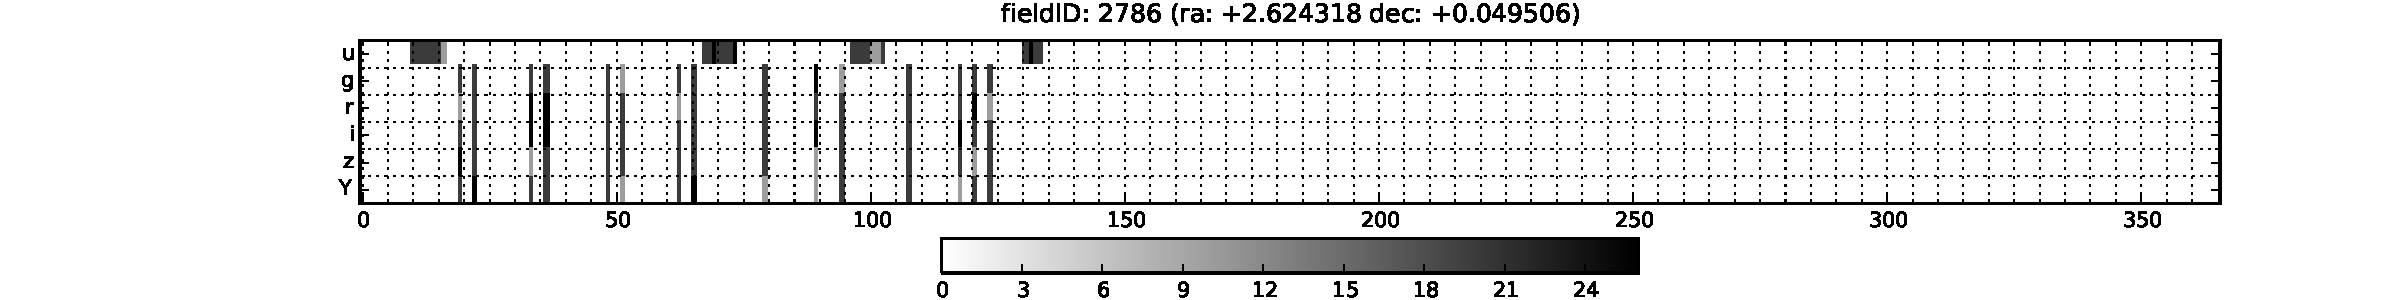
\includegraphics[width=\textwidth]{figs/supernova/fig_firstSeason_1}
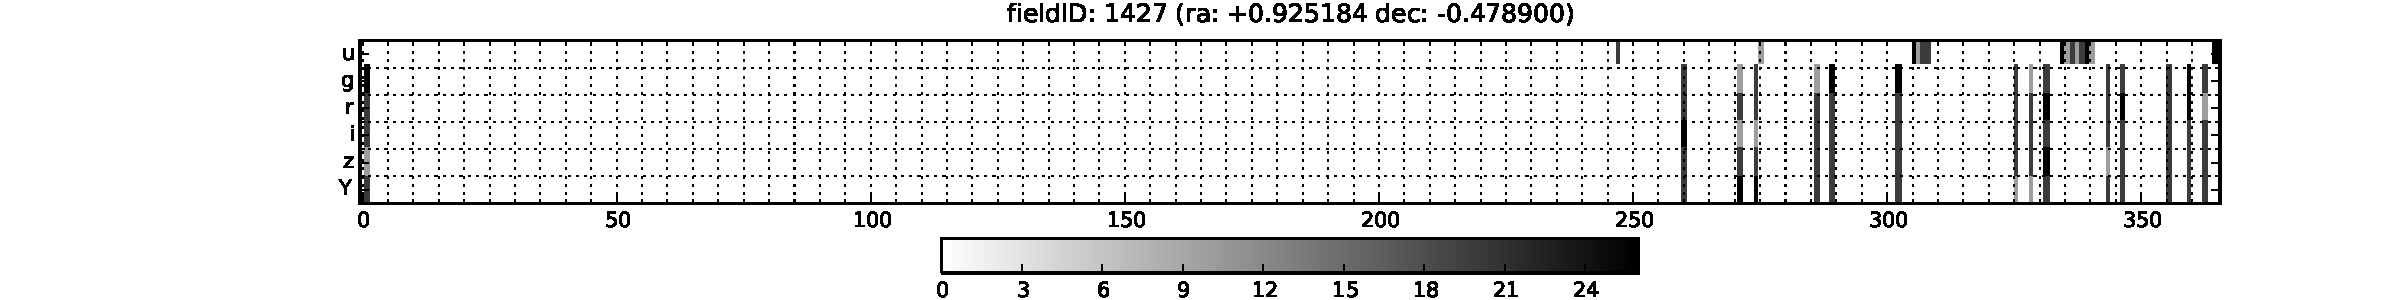
\includegraphics[width=\textwidth]{figs/supernova/fig_firstSeason_2}
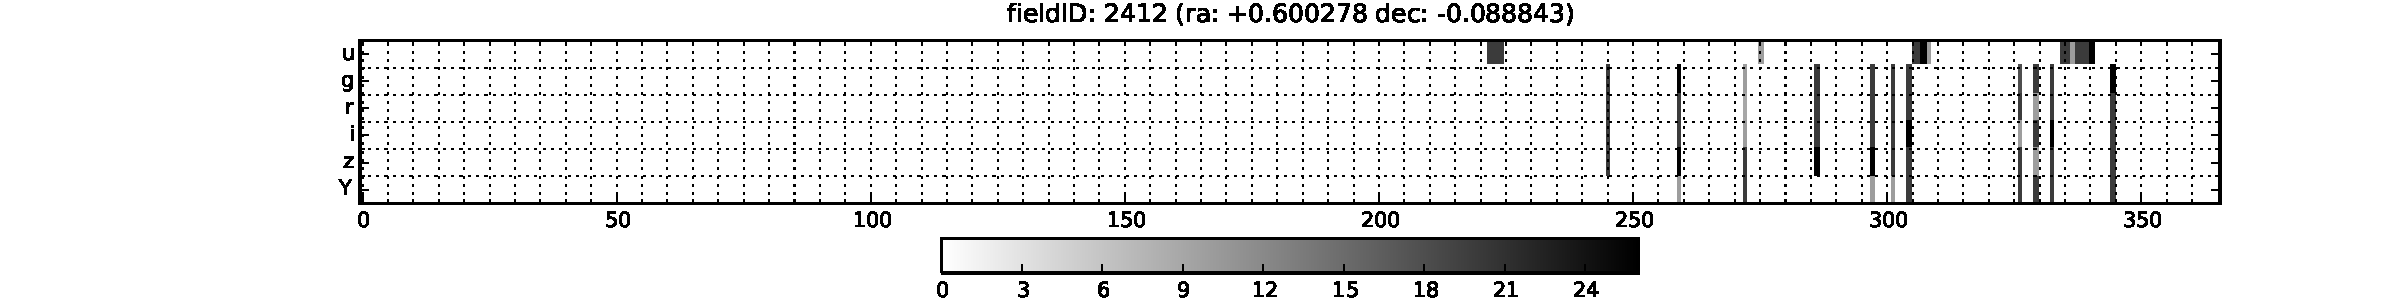
\includegraphics[width=\textwidth]{figs/supernova/fig_firstSeason_3}
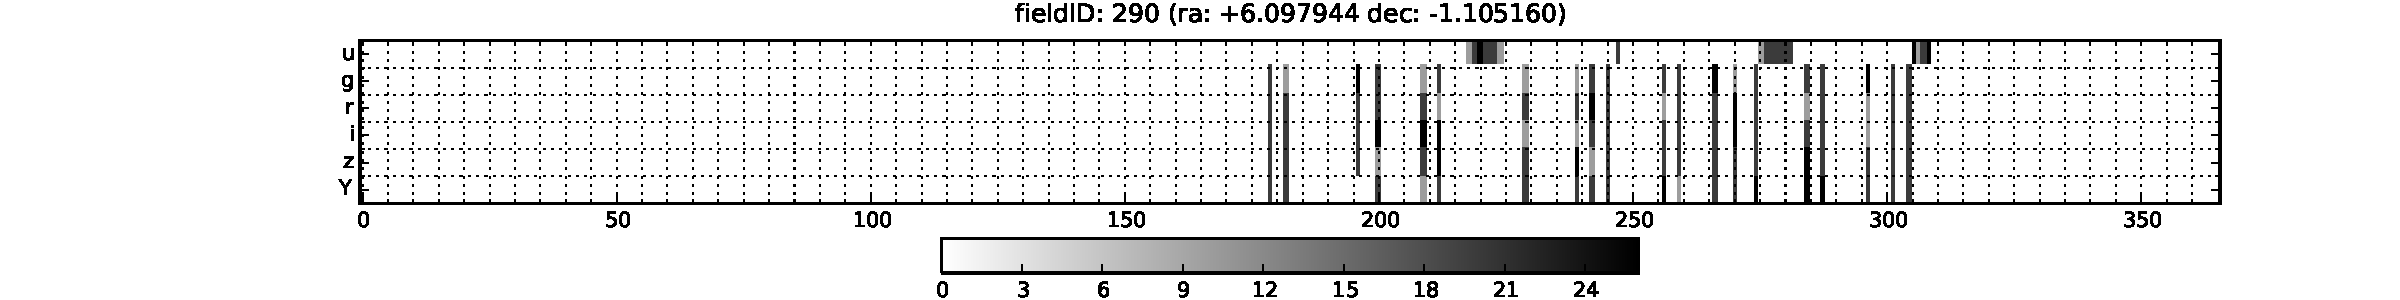
\includegraphics[width=\textwidth]{figs/supernova/fig_firstSeason_4}
\label{fig:opsimSummary}
\caption{Cadence in different filters for a few LSST DDFs in
    the the ouptut of OpSim version Enigma 1189. This ignores issues of chip 
gaps and overlaps between LSST pointings. These issues have been addressed in \citep{CarrollEtal2014} and Awan et.al. (2015, in prep.). We will add these to this analysis.}
\end{figure}



% --------------------------------------------------------------------

\subsection{Discussion}
\label{sec:keyword:discussion}

Discussion: what risks have been identified? What suggestions could be
made to improve this science project's figure of merit, and mitigate
the identified risks?


\begin{itemize}
\item Intrinsic Dispersion, environmental effects, newer analysis methods
\item Follow-up procedures: What is feasible? Where will our training samples for classification and light curve models come from (other experiments, our own 
sub-samples with spectroscopic follow-up?), spectroscopic follow-up of host galaxies. Can hosts be identified?
\item `Systematics': In what ways will the real data not match the assumptions made in analysis. Having a large sample of SN, to understand the astrophysics would be useful for this. 
\end{itemize}


% ====================================================================

\navigationbar


% --------------------------------------------------------------------

\chapter[Deep Drilling Fields]{Drilling Deep: Options for a Small Number of Enhanced Observation
Fields}
\def\chpname{deepdrilling}\label{chp:\chpname}

Chapter editors:
\credit{nielbrandt},
\credit{rhiannonlynne}.

% --------------------------------------------------------------------

\section{Introduction}
\label{sec:\chpname:intro}

% Introduce, with a very broad brush, this chapter's science projects,
% and why it makes sense for them to be considered together.

% Individual sections go below, one science project per section, one
% section per file.

% --------------------------------------------------------------------

% \input{DDsection1}

% --------------------------------------------------------------------

% \input{DDsection2}

% --------------------------------------------------------------------


% --------------------------------------------------------------------

\chapter[Special Surveys]{Special Surveys}
\def\chpname{specialsurveys}\label{chp:\chpname}

%\noindent {\it
%Knut Olsen, David Nidever
%}

% Confirmed leads for LMC/SMC: Knut Olsen, David Nidever

% Confirmed leads for special surveys:

% --------------------------------------------------------------------

\section{Introduction}
\label{sec:specials:intro}

% Introduce, with a very broad brush, this chapter's science projects,
% and why it makes sense for them to be considered together.

Includes: science programs not served effectively by the main
wide-fast-deep program; additional sky regions; special cadences;
candidate commissioning surveys

% Add sections below, one science investigation per section, one
% section per file.
% --------------------------------------------------------------------

% ====================================================================

\chapter{The Magellanic Clouds}
\def\chpname{MCs}\label{chp:\chpname}

Chapter Editors:
\credit{dnidever},
\credit{knutago}

% \section*{Summary}
% \addcontentsline{toc}{section}{~~~~~~~~~Summary}
%
% Executive summary goes here, highlighting the primary conclusions from
% the chapter's science cases. This should be abstract length, no more:
% say, 200 words.

\section{Introduction}

The Magellanic Clouds have always had outsized importance for
astrophysics.  They are critical steps in the cosmological distance
ladder, they are a binary galaxy system with a unique interaction
history, and they are laboratories for studying all manner of
astrophysical phenomena.  They are often used as jumping-off points
for investigations of much larger scope and scale; examples are the
searches for extragalactic supernova prompted by the explosion of
SN1987A and the dark matter searches through the technique of
gravitational microlensing.  More than 17,000 papers in the NASA ADS
include the words ``Magellanic Clouds'' in their abstracts or as part
of their keywords, highlighting their importance for a wide variety of
astronomical studies.

An LSST survey that did not include coverage of the Magellanic Clouds
and their periphery would be tragically incomplete.  LSST has a unique
role to play in surveys of the Clouds.  First, its large $A\Omega$
will allow us to probe the thousands of square degrees that comprise
the extended periphery of the Magellanic Clouds with unprecedented
completeness and depth, allowing us to detect and map their extended
disks, stellar halos, and debris from interactions that we already
have strong evidence must exist.  Second, the ability of LSST
to map the entire main bodies in only a few pointings will allow us to
identify and classify their extensive variable source populations with
unprecedented time and areal coverage, discovering, for example,
extragalactic planets, rare variables and transients, and light echoes
from explosive events that occurred thousands of years ago (REFS).
Finally, the large number of observing opportunities that the LSST
10-year survey will provide will enable us to produce a static imaging
mosaic of the main bodies of the Clouds with extraordinary image
quality, an invaluable legacy product of LSST.

We have several important scientific questions:
\begin{enumerate}

\item What are the stellar and dark matter mass profiles of the
Magellanic Clouds?  To answer this we need to map their extended disks, halos, debris, and streams.  We can use
streams and RR Lyrae stars as probes of the 3D mass profile.

\item What is the satellite population of the Magellanic Clouds? The
discovery of dwarf satellites by the Dark Energy Survey and other
surveys hint at LSST's potential here.

\item What are the internal dynamics of the Magellanic Clouds?  Proper
motions from HST and from the ground have measured the bulk
motions of the Clouds and have, in combination with spectroscopy,
begun to unravel the three dimensional internal dynamics of the
Clouds.

\item How do exoplanet statistics in the Magellanic Clouds compare to
those in the Milky Way?  The calculations in the next section show that
LSST can measure transits of Jupiter-like planets, an intriguing
prospect given the Clouds' lower metallicity environment.

\item What are the variable star and transient population of the Clouds?
LSST will enable population studies, linking star formation and chemical
enrichment histories.

\item What can we learn about supernovae and other explosive events from
their light echoes?  Echoes can give view of such events unavailable by
any other means.

\end{enumerate}


These questions can be grouped into main overarching science themes:
\begin{enumerate}
\item {\bf Galaxy formation evolution}: The study of the formation and
evolution of the Large and Small Magellanic Clouds (LMC and SMC,
respectively), especially their interaction with each other and the
Milky Way. The Magellanic Clouds (MCs) are a unique local laboratory
for studying the formation and evolution of dwarf galaxies in
exquisite detail.  LSST's large FOV will be able to map out the
three-dimensional structure, metallicity and kinematics in great
detail.
\item {\bf Stellar astrophysics \& Exoplanets}:  The MCs have been
used for decades to study stellar astrophysics, microlensing and other
processes.  The fact that the objects are effectively all at a single
known distance makes it much easier to study them than in, for
example, the Milky Way.  LSST will extend these studies to fainter
magnitudes, higher cadence, and larger area.
\end{enumerate}

Many different types of objects and measurements with their own
cadence ``requirements'' will fall into these two broad categories
(with some overlap).
% These will be outlined in the next section.
A very important aspect of the ``galaxy evolution'' science theme is
not just the cadence but also the sky coverage of the Magellanic
Clouds ``mini-survey.''  A common misunderstanding is that the MCs
only cover a few degrees on the sky.  That is, however, just the
central regions of the MCs akin to the thinking of the Milky Way as
the just the bulge.  The full galaxies are actually much larger with
LMC stars detected at $\sim$21$^{\circ}$ ($\sim$18 kpc) and SMC stars
at $\sim$10$^{\circ}$ ($\sim$11 kpc) from their respective centers.
The extended stellar debris from their interaction likely extends to
even larger distances.  Therefore, to get a complete picture of the
complex structure of the MCs will require a mini-survey that covers
$\sim$2000 deg$^2$.
% At this point, it not entirely clear how to
% include this into the metrics.
Note, that for the second science case
this is not as much of an issue since the large majority of the
relevant objects will be located in the high-density, central regions
of the MCs.

Our investigation of how the LSST observing strategy will affect the
science outline here is still in its infancy. Some of the disgnostic and
figure of merit metrics developed elsewhere in this paper may be useful
for assessing the Magellanic Cloud science cases as well. In the
meantime we present below two science cases in the early stages of development that show some of the promise LSST shows in this area.

% static science vs. variables
% cadence vs. areal coverage
%  -want to cover whole SCP area to some necessary depth
%  -cadence for time-variable objects in full area or portion
%    what's the minimal # of visits (with decent phase coverage) to do this?  ask Kathy
%    Paula Szkody white paper on doing the full MCs for variables, linked to old MC cadence page
%   maybe a separate metric for spatial structure
%   -variabes:  ability to recover period, classify,


% --------------------------------------------------------------------
%
% \new{Below is a generic list of things we want to measure in the
% Magellanic Clouds.}
% % These will need to be divided among a small set of
% % science sections, each describing a focused science project that has a
% % figure of merit, that is a function of various diagnostic metrics. The
% % final version of the chapter tex file probably will not contain this
% % list.
%
% \begin{enumerate}
%
% \item Deep Color Magnitude Diagrams
% %  -Deep CMDs, just a matter of number of visits
% %  -do the full SMASH (and relevant DES area) with full spatial coverage, at least to SMASH depths, smaller
% %  number of epochs, ~5 sigma at gri~25
% % Knut thoughts: I think we want to make sure that we get 1 mag below old turnoff out to 100 kpc in ugriz with 10sigma precision, i.e. ugriz~25
%
%
% \item Proper Motions
% %-Proper Motions, cadence not as much of an issue, just more epochs
% %  bulk proper motion
% %  LMC spiral motion, streaming motions
% %  internal velocity dispersion
%
%
% %\item Parallaxes
% %-Parallaxes, also mostly a function of nubmer of epochs
% %  bulk distances
% %  internal distance spread
% %  -probably not get parallaxes at MC distances, but could do foreground rejection
%
% \item Variable stars
%
% %-Variables, RR Lyrae, Cepheids might be too bright, dwarf cepheids/scuti good, many more of them.
% %   especially good for getting the 3D structure (out to large distances) of the MCs
% %   -eclipsing binaries (get very accurate distances, see OGLE paper), pulsating WDs, CVs, T Tauri stars
% % novae, supernovae  in Paula's white paper
%
% % use MCs are a way to get templates for variable sources that LSST will detect all over the sky
% % look at variable group metrics
%
%
% \item Transients
% %-Transients, dwarf novae
% % Mike Lund will work on some text for this.  Also did work on cadence considerations
% % for detecting periodic objects in general (periodogram purity function).
%
% \item Transiting Exoplanets
% % -Transiting planets, Mike Lund
% % -need deep drilling to have any hope of finding them
% % -best between ~0.8-1.6 Msun to detect exoplanets, not too faint
% % -can't get ingress/egress but can detect the dip and periodicity
% %   that's enough to characterize
% % -challenging to do follow-up because they are quite faint and too many (?)
% % -cadence?  cover all timescales properly
% % -what's the expected period distribution
%
% % See Lund et al.\ (2015) and the exoplanet discussion in previous part
% % of this paper.
%
% % PASP
%
% %\item Astrometric binaries
% %-Astrometric binaries
%
% \item Light-echoes
% % it's a surface-brightness issue, can see fainter things with LSST than MOSAIC/DECAM
% % could trace out lightcurve if more epochs
%
% \item Gyrochronology
% %-Gychronology, need to get periods of the dwarfs, gives age information
% %  -gyro periods are ~10 days at 1 Gyr and ~30 days at 10 Gyr
%
% \item Interstellar scintillation
% % run in movie mode for 1-2 nights to find missing molecular gas (H2)
% % https://github.com/LSSTScienceCollaborations/ObservingStrategy/issues/68
%
% % Legacy survey
% % use the best seeing to get great data on the MC main bodies
%
% %\item Astroseismology
% %-Astroseismology, dwarfs/giants, giants vary by a couple percent and on "longer" timescales, but
% %    probably too bright for LSST, OGLE probably has best data for those. however LSST might be able to do
% %    asteroseismology of giants to larger distances, measure masses/ages of halo giants!
% %    dwarfs are harder because they vary less and need more higher frequency observations
%
% \end{enumerate}
%
%
% ====================================================================

% PJM: moved to Future Work while MAF analysis is pending:
% % ====================================================================
%+
% SECTION:
%    MCs_ProperMotion.tex
%
% CHAPTER:
%    magclouds.tex
%
% ELEVATOR PITCH:
%-
% ====================================================================

% \section{The Proper Motion of the LMC and SMC}
\subsection{The Proper Motion of the LMC and SMC}
\def\secname{\chpname:propermotion}\label{sec:\secname}

\credit{dnidever},
\credit{knutago}

In the last decade work with $HST$ has been able to measure the bulk
tangential (in the plane of the sky) velocities ($\sim$300 km/s) of
the Magellanic Clouds (Kallivayalil et al.\ 2016a,b,2013) and even the
rotation of the LMC disk \citep{2014ApJ...781..121V}. Gaia
will measure precise proper motions of stars to $\sim$20th magnitude
which will include the Magellanic red giant branch stars. LSST will be
complementary to Gaia and measure proper motions of stars in the
$\sim$20--24 mag range that includes Magellanic main-sequence stars
which are far more numerous than giants, and, therefore, more useful
for mapping extended stellar structures. The LSST 10-year survey
proper motion precision will be $\sim$0.3--0.4 mas/yr at LMC
main-sequence turnoff at r$\approx$22.5--23.  This will allow for
accurate measurement of proper motions of {\em individual stars} at the
$\sim$5$\sigma$ level.

Besides measuring kinematics, the LSST proper motions can be used to
produce clean samples of Magellanic stars.
%  clean samples of background
% galaxies (no proper motions) and this is commonly done with $HST$ data
% of
%
In addition, LSST proper motions can be used to improve star/galaxy
separation which is quite significant for faint, blue Magellanic
main-sequence stars.

% streaming motions

% can we do individual LMC stars with LSST, or small groups?

% SRD says want 0.2 mas/yr accuracy over the course of the survey
% 0.2 mas/yr at r=20.5 (similar to Gaia)
% ~0.25 mas/yr at r=22
% ~0.3 mas/yr at r=22.5 LMC turnoff
% ~0.4 mas/yr at r=23
% 1 mas/yr for r=24
% See Figure 21 from Ivezic et al. (2012) or slide 46 of overview-sci-reqs.pdf
%have the astrometric precision to measure the proper motions of individual
%Proper motion cleaning to find the giants?? gaia does that already
%lsst can use proper motion cleaning to do star/galaxy separation as well
%
%The
%The Magellanic Clouds have a large tangential velocity (in the plane of the sky) that has been
%Gaia will be able to see the bright stuff, need lsst to get the MSTO
%gaia/lsst synergy
%
%metric that calculates the proper motion accuracy of LMC MSTO stars at r=23 and calculates the sigma-level of
%the proper motion measurement (2.0 mas/yr / sigma_pm ).

% --------------------------------------------------------------------

% \subsection{Metrics}
\subsubsection{Metrics}
\label{sec:\chpname:metrics}

The natural Figure of Merit for this science case is the precision
with which the proper motion of the Magellanic Clouds can be measured.
This is likely to depend on the following diagnostic metrics:

% metric on surface brightness limit in different parts of the sky
% to MC structure
% could use metric for how much of the Besla stellar debris we can detect
%  even just that region of the sky covered

\begin{itemize}

\item  Single star proper motion precision, possibly quantified as.
the significance level
($\sigma$-level) of the proper motion measurement of one Magellanic MSTO
star (r=23 mag). We would expect this to take values of
$\sim$2.0 mas yr$^{-1}$ / $\sigma_{\rm pm}$.
%  the precision proper motion metric that
%  Metric that calculates the proper motion accuracy of LMC MSTO stars at r=23 and calculates the sigma-level of
%the proper motion measurement (2.0 mas/yr / sigma_pm ).

\item Another useful diagnostic metric would be the surface
brightness limit of the Magellanic structures, using MSTO stars.

\item A metric quantifying how much of the expected Magellanic debris/structure
\citet[from][]{2012MNRAS.421.2109B} model) we can detect would allow the
proper motion science case to be extended to peripheral structures.
This would depend
mostly on the area covered, but we could also use the surface
brightness limit (calculated above) directly.

\end{itemize}

% % --------------------------------------------------------------------
%
% \subsection{Metrics}
% \label{sec:\secname:metrics}
%
% % --------------------------------------------------------------------
%
% \subsection{OpSim Analysis}
% \label{sec:\secname:analysis}
%
% % --------------------------------------------------------------------
%
% \subsection{Discussion}
% \label{sec:\secname:discussion}
%
% ====================================================================
%
% \subsection{Conclusions}
%
% Here we answer the ten questions posed in
% \autoref{sec:intro:evaluation:caseConclusions}:
%
% \begin{description}
%
% \item[Q1:] {\it Does the science case place any constraints on the
% tradeoff between the sky coverage and coadded depth? For example, should
% the sky coverage be maximized (to $\sim$30,000 deg$^2$, as e.g., in
% Pan-STARRS) or the number of detected galaxies (the current baseline but
% with 18,000 deg$^2$)?}
%
% \item[A1:] ...
%
% \item[Q2:] {\it Does the science case place any constraints on the
% tradeoff between uniformity of sampling and frequency of  sampling? For
% example, a rolling cadence can provide enhanced sample rates over a part
% of the survey or the entire survey for a designated time at the cost of
% reduced sample rate the rest of the time (while maintaining the nominal
% total visit counts).}
%
% \item[A2:] ...
%
% \item[Q3:] {\it Does the science case place any constraints on the
% tradeoff between the single-visit depth and the number of visits
% (especially in the $u$-band where longer exposures would minimize the
% impact of the readout noise)?}
%
% \item[A3:] ...
%
% \item[Q4:] {\it Does the science case place any constraints on the
% Galactic plane coverage (spatial coverage, temporal sampling, visits per
% band)?}
%
% \item[A4:] ...
%
% \item[Q5:] {\it Does the science case place any constraints on the
% fraction of observing time allocated to each band?}
%
% \item[A5:] ...
%
% \item[Q6:] {\it Does the science case place any constraints on the
% cadence for deep drilling fields?}
%
% \item[A6:] ...
%
% \item[Q7:] {\it Assuming two visits per night, would the science case
% benefit if they are obtained in the same band or not?}
%
% \item[A7:] ...
%
% \item[Q8:] {\it Will the case science benefit from a special cadence
% prescription during commissioning or early in the survey, such as:
% acquiring a full 10-year count of visits for a small area (either in all
% the bands or in a  selected set); a greatly enhanced cadence for a small
% area?}
%
% \item[A8:] ...
%
% \item[Q9:] {\it Does the science case place any constraints on the
% sampling of observing conditions (e.g., seeing, dark sky, airmass),
% possibly as a function of band, etc.?}
%
% \item[A9:] ...
%
% \item[Q10:] {\it Does the case have science drivers that would require
% real-time exposure time optimization to obtain nearly constant
% single-visit limiting depth?}
%
% \item[A10:] ...
%
% \end{description}

% ====================================================================
%
% \navigationbar


% ====================================================================

% ====================================================================
%+
% SECTION:
%    MCs_FutureWork.tex
%
% CHAPTER:
%    transients.tex
%
% ELEVATOR PITCH:
%    Ideas for future metric investigation, with quantitaive analysis
%    still pending.
%-
% ====================================================================

\section{Future Work}
\def\secname{\chpname:future}\label{sec:\secname}

In this section we provide a short compendium of science cases that
are either still being developed, or that are deserving of quantitative
MAF analysis at some point in the future.

% ====================================================================

\input{MagellanicClouds/MCs_ProperMotion.tex}

% ====================================================================

\input{MagellanicClouds/MCs_Exoplanets.tex}

% ====================================================================


% ====================================================================


% --------------------------------------------------------------------

% \input{special2}

% --------------------------------------------------------------------

\navigationbar


% --------------------------------------------------------------------

\chapter[Tensions and Trade-offs]{Tensions and Trade-offs}
\def\chpname{tradeoffs}\label{chp:\chpname}

\noindent {\it
...
}

Discussion and conclusions chapter, at the end, highlighting the
issues that we will need to figure out. Possible topics include the
cost/benefit tradeoffs between competing objectives.


% --------------------------------------------------------------------

\bibliographystyle{apj}
\bibliography{references}

% --------------------------------------------------------------------

\end{document}

% ====================================================================
